%\documentclass[11pt,a4paper,oneside]{book}
%\usepackage[hmargin={1.25in,1.25in},vmargin={1.25in,1.25in}]{geometry}




\documentclass[12pt,a4paper,oneside]{book}
\usepackage{setspace}
\onehalfspacing
\usepackage[hmargin={2.5cm,2.5cm},vmargin={2.5cm,2.5cm}]{geometry}


\usepackage[french]{babel}
\usepackage[utf8]{inputenc}
\usepackage[T1]{fontenc}

\usepackage{graphicx}

\usepackage[final]{pdfpages} % include pdf files

\usepackage{amsthm}
\usepackage{amsmath}
\usepackage{amsfonts}
\usepackage{tabularx}
\usepackage[nottoc, notlot, notlof, numbib, numindex]{tocbibind}
\usepackage{charter}


\usepackage{url}
%\usepackage{geometry}
\usepackage{enumitem}
\usepackage{hyperref}
\usepackage{comment}
\usepackage{listings} 
\usepackage{caption} 
\usepackage{stmaryrd}
\usepackage{fancybox}
\usepackage{makeidx}

\usepackage{color}

\usepackage{mdframed}

\definecolor{bg}{cmyk}{0,0,0,0.03}


\usepackage{minted}

\definecolor{bookColor}{cmyk}{0 ,0 ,0 ,1} \color{bookColor}

%\usemintedstyle{bw}
 


\newcounter{nalg}[chapter] % defines algorithm counter for chapter-level
\renewcommand{\thenalg}{\thechapter .\arabic{nalg}} %defines appearance of the algorithm counter
\DeclareCaptionLabelFormat{algocaption}{\textsc{Algorithme} \thenalg} % defines a new caption label as Algorithm x.y


\lstnewenvironment{algorithm}[1][] %defines the algorithm listing environment
{   
    \refstepcounter{nalg} %increments algorithm number
    \captionsetup{labelformat=algocaption,labelsep=colon} %defines the caption setup for: it ises label format as the declared caption label above and makes label and caption text to be separated by a ':'
    \lstset{ %this is the stype
        frame=tB,
        numbers=left, 
        numberstyle=\small,
        basicstyle=\small, 
        keywordstyle=\color{black}\bfseries\em,
        keywords={,input, output, return, then, endif, datatype, function, in, if, else, foreach, while, begin, end, repeat, until,} %add the keywords you want, or load a language as Rubens explains in his comment above.
        numbers=left,
        xleftmargin=.04\textwidth,
        #1 % this is to add specific settings to an usage of this environment (for instnce, the caption and referable label)
    }
}
{}

\def\lstlistingautorefname{Algorithme}




\graphicspath{{graphes/}}



\newtheoremstyle{break}  % follow `plain` defaults but change HEADSPACE.
  {\topsep}   % ABOVESPACE
  {\topsep}   % BELOWSPACE
  {}  % BODYFONT
  {0pt}       % INDENT (empty value is the same as 0pt)
  {\bfseries} % HEADFONT
  {.}         % HEADPUNCT
  {\newline}  % HEADSPACE. `plain` default: {5pt plus 1pt minus 1pt}
  {}          % CUSTOM-HEAD-SPEC
\theoremstyle{break}
\newtheorem{defin}{Définition}[chapter]
\def\definautorefname{Définition}
\newtheorem{exem}{Exemple}[chapter]
\def\exemautorefname{Exemple}


\newtheoremstyle{breakplain}  % follow `plain` defaults but change HEADSPACE.
  {\topsep}   % ABOVESPACE
  {\topsep}   % BELOWSPACE
  {\itshape}  % BODYFONT
  {0pt}       % INDENT (empty value is the same as 0pt)
  {\bfseries} % HEADFONT
  {.}         % HEADPUNCT
  {\newline}  % HEADSPACE. `plain` default: {5pt plus 1pt minus 1pt}
  {}          % CUSTOM-HEAD-SPEC
\theoremstyle{breakplain}
\newtheorem{theo}{Théorème}[chapter]
\def\theoautorefname{Théorème}
\newtheorem{lem}{Lemme}[chapter]
\def\lemautorefname{Lemme}
\newtheorem{prop}{Proposition}[chapter]
\def\propautorefname{Proposition}

\addto\captionsfrench{\def\tablename{{\textsc{Tableau}}}}


\newcommand{\printcode}[1]{

\begin{mdframed}[linecolor=black, topline=true, bottomline=true,
  leftline=false, rightline=false, backgroundcolor=bg]
\inputminted[linenos, breaklines, breakbytokenanywhere,fontfamily=courier,]{python}{#1}
\end{mdframed}
}


\makeindex

\begin{document}
%\maketitle

\begin{titlepage}
\noindent \begin{minipage}{0.83\textwidth}
\noindent \textbf{UNIVERSIT\'E LIBRE DE BRUXELLES}\hfill{}\\
\textbf{Faculté des Sciences}\hfill{}\\
\textbf{Département d'Informatique}\hfill{}
\end{minipage}
\begin{minipage}{0.17\textwidth}
\includegraphics[keepaspectratio=true,width=\textwidth]{images/ulbboxlogoBW.pdf}
\end{minipage}
\begin{center}
\vfill{}\vfill{}\vfill{}
%\begin{center}
{\Huge Test d'ordonnançabilité pour systèmes à\\criticité~mixte~par~exploration~d'automates}
%\end{center}
{\Huge \par}
\begin{center}{\LARGE Simon \textsc{Picard}}\end{center}{\Huge \par}
%\vfill{}\vfill{}\vfill{}\vfill{}\vfill{}
\vfill{}
\includegraphics[keepaspectratio=true,width=\textwidth-2cm]{images/ulb.pdf}
\vfill{}
\begin{flushright}{\large \textbf{Promoteurs :}}\hfill{}{\large Mémoire présenté en vue de}\\
{\large Prof. Gilles \textsc{Geeraerts}}\hfill{}{\large l'obtention du grade de}\\{\large Prof. Joël \textsc{Goossens}}
\hfill{}{\large Master en Sciences Informatiques}\end{flushright}{\large\par}
\vfill{}\vfill{}\enlargethispage{2cm}
\textbf{Année académique 2015~-~2016}
\end{center}
\end{titlepage}



\newpage
%\newgeometry{hmargin={3.5cm,1.5cm},vmargin={2.5cm,2.5cm}}
\thispagestyle{empty} 
\null

\frontmatter


\chapter*{Résumé}
Ce mémoire propose un test d'ordonnançabilité CM exact pour un système de tâches CM périodiques ou sporadiques avec un algorithme donné.\\
La solution de ce problème se base sur une réduction de celui-ci vers l'accessibilité dans un automate fini. Cette solution est ensuite améliorée pour les systèmes de tâches CM sporadiques grâce à la définition d'une relation de simulation.\\

La première partie du mémoire présente toutes les notions nécessaires pour la compréhension du travail fourni : l'ordonnancement temps réel, l'ordonnancement en criticité mixte, un automate fini, l'accessibilité et les antichaînes basées sur une relation de simulation.\\

Ensuite, une présentation des algorithmes d'ordonnancement CM pour tâches CM sporadiques est faite, en insistant sur leur condition suffisante d'ordonnançabilité. Les algorithmes présentés sont \textit{Vestal}, \textit{OCBP} et ses extensions, \textit{EDF-VD}, \textit{Greedy} et un algorithme original inspiré de \textit{LLF} est proposé : \textit{LWLF}.\\

Le chapitre suivant offre une représentation de l'ordonnancement CM d'un système de tâches CM périodiques et sporadiques selon un algorithme sous forme d'automate fini.\\
Ensuite, la relation de simulation de tâches oisives est présentée.\\

Par la suite, deux comparaisons sont mises en évidence. La première tient de la complexité du problème d'accessibilité basé sur l'ordonnancement CM de tâches CM périodiques ou sporadiques selon un algorithme, avec et sans antichaîne.\\
La seconde se concentre sur l'ordonnançabilité des différents algorithmes d'ordonnancement présenté plus tôt dans le mémoire.\\

Enfin, les conclusions du travail discutent des résultats et offrent des propositions de travaux ultérieurs.


\chapter*{Remerciements}
Je tiens à remercier l'Université Libre de Bruxelles, mon Alma Mater, pour m'avoir offert l'accès à un enseignement de qualité durant ces cinq dernières années.\\

Je tiens à remercier les promoteurs de ce mémoire pour m'avoir proposé le sujet de ce dernier, pour m'avoir guidé durant mon travail et pour leur convivialité.

En particulier, je tiens à remercier Gilles Geeraerts pour le cours qu'il m'a enseigné en premier bachelier, \textit{Fonctionnement des ordinateurs}. La qualité de son enseignement a permis de confirmer ma passion pour les sciences informatiques.

Je tiens à remercier Joël Goossens, pour la précision de son cours \textit{Operating systems II} avec lequel j'ai fait la rencontre de l'ordonnancement temps réel, notion majeure dans ce mémoire.\\

Je tiens à remercier Emmanuel Filiot, membre du jury pour ce mémoire. Il a été choisi pour l'adéquation de ses travaux au sujet et, car c'est avec son cours \textit{Informatique fondamentale} que j'ai fait la connaissance des méthodes formelles.\\

Je tiens à remercier Janine Hamel pour la relecture attentive qu'elle a faite de ce mémoire. Ses qualités en matière de syntaxe, d'orthographe, de grammaire, de ponctuation et de style m'ont grandement aidé pour la réalisation de ce travail.\\

Je tiens à remercier le Cercle Informatique, association étudiante aux multiples facettes. Véritable incubateur de personnalité, il m'a permis de m'épanouir aussi bien socialement qu'intellectuellement durant mon cursus et de développer mes qualités en gestion de groupes ainsi que de projets.\\

Je tiens à remercier Alice Picard, ma sœur, pour son soutien constant et inébranlable. Ses valeurs et son caractère font d'elle le féal idéal.\\

Je tiens à remercier mes parents pour l'amour et le temps qu'ils m'ont données.

En particulier, je tiens à remercier Isabelle Primo, ma mère, pour la stabilité qu'elle m'a offerte. J'ai toujours pu compter sur elle et je ne doute pas que ça continuera. Sa gentillesse a initié l'attention que j'ai pour le bien-être des autres.

Je tiens à remercier Éric Picard, mon père, pour les valeurs qu'il m'a transmises. Les combats qu'il mène avec brio ne cessent de m'inspirer. Sa contribution à la création de l'esprit autonome et débrouillard dont je bénéficie est non négligeable.\\

Je tiens à remercier Nadine Picard, Mamette, ma grand-mère, pour l'attention qu'elle n'a cessé de me porter. Sa joie de vivre à toute épreuve est pour moi un idéal auquel j'aspire.



\tableofcontents

\mainmatter

\chapter{Introduction}
Ce mémoire a été réalisé dans le cadre du second cycle d'études à l'Université Libre de Bruxelles en sciences informatiques. Ce travail est réalisé sous la direction des professeurs Gilles Geeraerts et Joël Goossens.\\

Les appareils informatiques que nous utilisons tous les jours sont pensés de telle sorte qu'ils supportent une multitude de fonctionnalités. Cette cohabitation de différents services se retrouve dans les \textit{smartphones}, sur les pages internet, sur un réveil matin, etc. Faire fonctionner plusieurs services en même temps n'est pas facile, car ils doivent se partager le processeur dont l'appareil sur lequel ils fonctionnent dispose. Il s'agit donc de donner à chacune de ces fonctionnalités du temps durant lequel elles pourront profiter du processeur, il faut \textit{ordonnancer} les fonctionnalités.\\

En plus de ces engins qui facilitent la vie, il y a ceux qui nous sauvent la vie, par exemple l'ABS d'une voiture, les radars des avions, les \textit{pacemakers}.\\
Pour cette seconde classe d'engins, il faut s'assurer que le comportement de leurs fonctionnalités soit correct. Il faut être sûr que leur exécution combinée est possible et assez rapide. Les programmes de ces appareils \textit{temps réel} doivent respecter des contraintes de temps. En effet, un ABS doit s'activer avec un délai minimal, sinon il ne servirait à rien.\\
L'ordonnancement temps réel a pour but d'agencer les différentes fonctionnalités d'un appareil temps réel, de sorte qu'elles respectent leur contrainte temporelle.\\
Différents algorithmes existent pour créer de tels agencements entre les fonctionnalités d'un appareil.\\

Aujourd'hui, de plus en plus d'appareils combinent des fonctionnalités \textit{critiques}, qui ne peuvent en aucun cas être défaillantes, et des services de commodité. Par exemple, un avion devra toujours s'assurer que son système de guidage fonctionne, alors que les télévisions des passagers pourraient être défaillantes, sans pour autant compromettre la sûreté de l'appareil volant.\\
C'est de ce constat qu'est né l'ordonnancement en \textit{criticité mixte}, un ordonnancement dans lequel toutes les fonctionnalités ne seraient pas égales. En effet, certaines seraient plus critiques que d'autres, et devraient toujours respecter leur contrainte temporelle, alors que ce n'est pas le cas pour fonctionnalités moins critiques.\\

L'ordonnancement en criticité mixte prend de plus en plus d'ampleur. Cet ordonnancement est plus compliqué que l'ordonnancement temps réel classique (en monoprocesseur).\\
À l'heure actuelle, à ma connaissance, il n'existe aucun moyen de déterminer avec certitude si, pour tout appareil avec des fonctionnalités de différentes criticités, il est ordonnançable sur monoprocesseur selon un certain algorithme, pour tout algorithme. En s'aidant des \textit{méthodes formelles}, ce mémoire répondra à cette question.

\chapter{État de l'art}
Ce chapitre présente l'état de l'art ayant pour sujet deux problèmes différents de deux domaines différents de l'informatique.\\
Premièrement, le chapitre se concentre sur l'ordonnancement à criticité mixte. Pour se faire, il faut commencer par introduire l'ordonnancement classique, puis une explication informelle de ce type d'ordonnancement est donnée, pour enfin terminer par le formalisme de celui-ci.\\
Dans un second temps, le problème de l'accessibilité est présenté, en commençant par fournir certaines notions de base, ensuite en exposant un formalisme pour finir par expliquer la notion d'antichaîne. Par la suite, l'interaction entre ces deux problèmes est mise au clair.\\
Enfin, les contributions  qui seront faites dans ce mémoire et sa structure seront détaillées.

\section{Ordonnancement de systèmes à criticité mixte}
\subsection{Notions élémentaires}
L'un des domaines majeurs de l'informatique théorique actuelle est celui de l'ordonnancement. Il s'agit d'organiser dans le temps la réalisation de différents travaux, compte tenu de contraintes temporelles. Pour s'exécuter, ces travaux ont besoin d'avoir accès à une ou plusieurs ressources partagées entre eux. En pratique, une fois qu'un travail est généré, il possède un temps d'exécution et une échéance. Dans la plupart des cas, on parle de système comprenant une série de travaux, le but est alors d'agencer ces différents travaux de sorte qu'ils ne ratent pas leurs échéances, il faut partitionner la ou les ressources partagées entre les travaux. L'objet de cette sous-section est de définir un certain modèle pour ce problème ainsi que d'introduire différentes notions de la théorie de l'ordonnancement.
\subsubsection{Modèle}
Pour permettre l'ordonnancement d'un système, un certain formalisme a été défini, cette partie le présente.\\

Commençons par une notion fondamentale, le travail. Il s'agit d'un ensemble d'opérations à effectuer nécessitant de prendre possession de la ou d'une des ressources partagées.\\

\begin{defin}[Travail \cite{goossens2014os}]
Un travail\index{travail} est représenté par un triplet : 
\begin{center}
$J_i \overset{def}{=} (r_i, d_i, c_i)$
\end{center}
\begin{itemize}
\item $r_i \in \mathbb{N}^{+}$ est l'instant auquel $J_i$ est généré.
\item $d_i \in \mathbb{N}^{+}$ est l'échéance absolue de $J_i$, c'est-à-dire le moment avant lequel le travail doit impérativement avoir été exécuté complètement. On assume que $d_i > r_i$
\item $c_i \in \mathbb{N}^{+}$ définit la durée d'exécution du travail.
\end{itemize}
Le travail $J_i$ doit donc recevoir $c_i$ unités de processeur durant l'intervalle $[r_i, d_i)$. $[a,b)$ est l'intervalle entre $a$ et $b$, $a$ est inclus et $b$ ne l'est pas. \\
En général, on parle d'instance\index{instance} $I$, il s'agit d'un ensemble de travaux : $ I = \{J_1, J_2, ...\} $
\end{defin}
Souvent, le programme à exécuter possède une partie d'opération récurrente, en particulier on considère les tâches périodiques et sporadiques.\\

\begin{defin}[Tâche périodique \cite{goossens1999scheduling}]
Une tâche périodique\index{tâche périodique} génère donc un nombre infini de travaux, elle est représentée par un quadruple :
\begin{center}
$\tau_i \overset{def}{=} (O_i, T_i, D_i, C_i)$
\end{center}
\begin{itemize}
\item $O_i \in \mathbb{N}^{+}$ est le décalage de la tâche, l'instant auquel le premier travail de la tâche est généré.
\item $C_i \in \mathbb{N}^{+}$ définit la durée d'exécution d'un travail généré par la tâche.
\item $D_i \in \mathbb{N}^{+}$ est l'échéance relative de la tâche, c'est donc le laps de temps entre la génération d'un travail et son échéance absolue.
\item $T_i \in \mathbb{N}^{+}$ est la périodicité de la tâche, c'est-à-dire l'intervalle entre deux générations de travail.\\
\end{itemize}
Le $k^{e}$ travail $J_{i,k}$ de la tâche $\tau_i$ est donc généré à l'instant $O_i + (k-1)*T_i$ et a pour échéance  $O_i+(k-1)*T_i+D_i$ .
\end{defin}

\begin{defin}[Tâche sporadique \cite{goossens1999scheduling}]
Une tâche sporadique\index{tâche sporadique} possède le même modèle que la tâche périodique, la différence est que $T_i$ ne représente plus la périodicité, mais le temps minimal entre deux générations de la tâche. La tâche sporadique est donc imprévisible.
\end{defin}

On définit ensuite une série caractéristique \cite{goossens1999scheduling} qu'une tâche peut avoir :
\begin{itemize}
\item Une tâche à échéance implicite\index{echeance implicite@échéance implicite} est une tâche où l'échéance correspond à la période, $D_i = T_i\ \forall i$
\item Une tâche à échéance contrainte\index{echeance contrainte@échéance contrainte} est une tâche où l'échéance est inférieure ou égale à la période, $D_i \le T_i\ \forall i$
\item Une tâche à échéance arbitraire\index{echeance arbitraire@échéance arbitraire} est une tâche où il n'y a pas de contraintes en la période et l'échéance de celle-ci.
\end{itemize}
On définit ensuite, sur un système\index{système de tâches} de plusieurs tâches $\tau = \{\tau_1, \tau_2, ...\}$
\begin{itemize}
\item Un système de tâches est synchrone\index{système de tâches!synchrone} si toutes ses tâches ont un décalage nul, $O_i = 0\ \forall i$
\item Asynchrone\index{système de tâches!asynchrone} sinon.
\end{itemize}

\subsubsection{Ordonnancement}
Une stratégie d'ordonnancement est un algorithme permettant le partage d'une ou plusieurs ressources entre plusieurs parties dont elles font la requête de manière simultanée et asynchrone \cite{goossens2014os}. Les ordonnanceurs sont utilisés, par exemple, dans un système d'exploitation, dans les disques durs, dans les routeurs internet ... Le but d'un ordonnanceur classique est d'éviter le gaspillage de ressources et de partager cette dernière de manière équitable entre ceux qui le demandent. Dans un ordonnanceur temps réel, une contrainte de temps doit être respectée, il faut que les processus se terminent avant leurs échéances, ce type d'ordonnanceur est largement utilisé dans les systèmes embarqués, par exemple dans un cardiostimulateur.\\

À l'heure actuelle, les constructeurs de systèmes embarqués ont tendance à implémenter plusieurs fonctionnalités sur une même plateforme pour réduire les coûts, la chaleur, l'alimentation... Malheureusement, un tel partage de ressources peut mener à des interférences entre les différents clients (entité voulant avoir accès aux ressources), on cherche donc à savoir si un tel ensemble de clients peuvent partager une ressource sans qu'il y ait de moments où un client n'a pas accès à cette ressource alors qu'il en a besoin.\\

Typiquement, on parle d'ordonnancement d'un processeur, on divise donc le temps d'exécution disponible grâce aux coups d'horloge, définissant le temps entre deux coups d'horloge successifs comme une unité de temps. L'ordonnanceur peut être préemptif, c'est-à-dire qu'il peut interrompre un travail pour en ordonnancer un autre.\\

Dans ce document, nous nous concentrerons sur les algorithmes d'ordonnancement préemptif sur un monoprocesseur à vitesse unitaire.\\

L'algorithme d'ordonnancement devra choisir, parmi plusieurs travaux, lequel pourra jouir de la puissance du processeur.  Pour ce faire, il utilisera un système de priorité clair et défini, chaque travail possédera une priorité et, en fonction de laquelle, l'ordonnanceur pourra partager le temps de calcul entre les travaux. Il existe trois classes d'algorithme d'ordonnancement \cite{goossens2014os} :\\

\begin{itemize}
\item Priorité fixe au niveau des tâches (Fixed Task Priority, FTP\index{FTP}) : il s'agit d'un ordonnancement où chaque tâche s'est vue attribuer une priorité avant l'exécution du système. Chaque travail hérite ensuite de la priorité de la tâche qui l'a générée.
\item Priorité fixe au niveau des travaux (Fixed Job Priority, FJP\index{FJP}) : chaque travail reçoit un niveau de priorité lorsqu'il est généré, celui-ci restera constant pour toute la durée du travail. Dès lors, différents travaux d'une même tâche peuvent avoir une priorité différente.
\item Priorité dynamique (Unrestructed Dynamic Priority, DP\index{DP}) : il s'agit du cas général où aucune contrainte ne s'applique à l'assignation des priorités aux travaux. En règle générale, cette nouvelle ligne conduite signifie qu'un travail va changer de priorité durant son existence.\\
\end{itemize}
On remarque que ces différentes classifications s'incluent elles-mêmes. En effet, FTP fait partie de la classe FJP qui est elle-même dans la classe DP.\\

L'ordonnancement est donc avant tout une certaine assignation de priorité. De manière générale, on considère que la valeur de la priorité attribuée à un travail est un naturel et est inversement proportionnel à sa priorité. Si deux travaux ont une même priorité, il faudra choisir de manière déterminée lequel sera ordonnancé. On définit donc la relation de priorité par le symbole $\succ$, par exemple : $\tau_i \succ \tau_j$, ici $\tau_i$ a une priorité supérieure à celle de $\tau_j$.\\

\pagebreak

\begin{defin}[Fonction de priorité \cite{santy2012ordonnancement}]
Formellement, une fonction de priorité\index{fonction de priorité} $\pi$ assigne à toute tâche $\tau_i$ d'un système de $n$ tâches $\tau$ (respectivement à tout travail $J_i$ d'une instance de $m$ travaux $I$) un nombre entier $\pi(\tau_i)$ (respectivement $\pi(J_i)$) compris entre $1$ et $n$ (respectivement $m$) qui représente de manière inversement proportionnelle la priorité de la tâche (respectivement du travail).
\begin{center}
$\pi : \tau \rightarrow \{0,...,n \}$\\
(Respectivement $\pi : I \rightarrow \{0,...,m \}$)\\
$\pi(\tau_i) < \pi(\tau_j) \Leftrightarrow \tau_i \succ \tau_j$\\
(Respectivement $\pi(J_i) < \pi(J_j) \Leftrightarrow J_i \succ J_j$)
\end{center}
\end{defin}

En temps réel, l'ordonnancement se porte en général sur un système de tâches. On souhaite prouver si un tel ensemble remplit les conditions introduites par ce mode. Deux nouvelles caractéristiques en émergent \cite{goossens2014os} :

\begin{itemize}
\item La faisabilité\index{faisabilité} d'un système de tâches est vérifiée s'il existe un certain partage du temps de calcul entre les différents travaux, de sorte que chacun d'entre eux ait pu exécuter toutes leurs actions sans rater leur échéance.
\item Un système de tâches est ordonnançable\index{ordonnançabilité} avec un certain algorithme d'ordonnancement si celui-ci permet d'agencer les travaux de sorte que chacun d'entre eux ait pu exécuter toutes leurs actions sans rater leur échéance.\\
\end{itemize}

Une définition analogue peut être faite pour une collection de travaux.\\

Il est à noter qu'il est possible dans certains cas qu'un système de tâches soit faisable, mais pas ordonnançable. Ces deux notions sont souvent liées à celle de l'utilisation qui représente la charge de travail du processeur : la quantité de travail effectué par rapport au temps dont il dispose pour le faire.\\

\begin{defin}[Utilisation \cite{goossens2014os}]
L'utilisation\index{utilisation} d'une tâche est définie par la fonction $U(\tau_i) \overset{def}{=} C_i/T_i$.\\
L'utilisation d'un système de tâches est la somme des utilisations des tâches le composant : $U(\tau) \overset{def}{=} \underset{\tau_i \in \tau}{\sum} (\tau_i)$
\end{defin}

Pour clôturer cette sous-section, un algorithme d'ordonnancement monoprocesseur est présenté. Il s'agit d'un algorithme à priorité statique au niveau des travaux (FJP) : EDF (Earliest Deadline First). Celui-ci attribue à chacun des travaux une priorité relative à leurs échéances absolues, plus elles sont proches, plus le travail est prioritaire. Formellement, on obtient $d_i < d_j \Leftrightarrow J_i \succ J_j$ et en cas d'égalité, $d_i = d_j \wedge i < j \Leftrightarrow J_i \succ J_j$.\\

\begin{theo}[\cite{goossens2014os}]
Si une collection de travaux est faisable, alors elle est ordonnançable avec EDF.
\end{theo}

EDF est donc un algorithme optimal pour un système de tâches à échéance implicite, synchrone ou asynchrone. Un algorithme est optimal\index{algorithme optimal} si l'agencement qu'il génère permet d'ordonnancer tout système de tâches d'un certain type.\\

\begin{theo}[\cite{liu1973scheduling}]
Pour un système de tâche périodique à échéance implicite $\tau$, celui-ci est faisable si et seulement si $U(\tau) \leq 1$
\end{theo}

\begin{figure}[h]
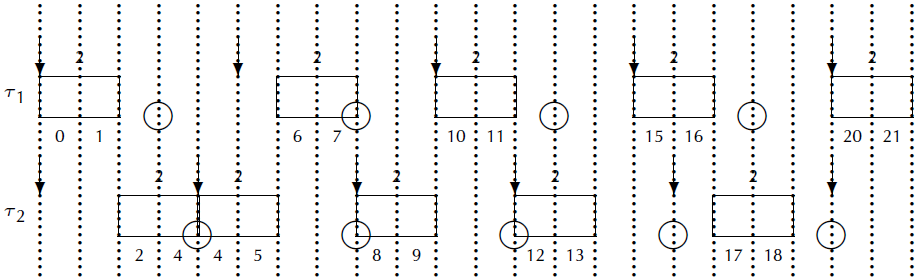
\includegraphics[width = \textwidth]{images/schedexample.png}
\caption{Représentation graphique d'un exemple d'ordonnancement par EDF \cite{goossens2014os}}
\label{edfsched}
\end{figure}

Il sera fréquent de représenter l'ordonnancement de travaux de manière graphique, la \autoref{edfsched} en est un exemple, ici il s'agit d'un système de deux tâches.
\begin{center}
$ \tau_1 = (0, 5, 3, 2) $\\
$ \tau_2 = (0, 4, 4, 2) $
\end{center}
Sur l'image :
\begin{itemize}
\item Chaque colonne en pointillé représente une unité de temps.
\item Une tâche est représentée sur une ligne
\item La flèche vers le bas représente la période de la tâche et donc le moment où le travail est généré
\item Un rond représente l'échéance d'un travail
\item Un carré représente l'exécution d'un travail durant une unité de temps
\end{itemize}

\pagebreak

\subsection{Criticité mixte}
\subsubsection{Définition informelle}
Le problème de criticité mixte est un problème d'ordonnancement. Pour rappel, il s'agit de gérer le partage d'un ensemble de ressources communes entre plusieurs clients.\\

Dans cette sous-section, nous nous penchons sur un problème plus précis : celui de la certification, dont le but est de prouver qu'un système est ordonnançable.\\

Précédemment, il a été présenté l'ordonnancement de travaux classique, ici on en déduit un nouveau problème où les clients pourraient avoir une importance plus ou moins élevée en fonction de leur criticité dans leur système. 
Il est évident que, dans une voiture, le système de freins ABS (<<Anti-lock Brake System>>) est plus important, plus critique que l'autoradio, car, en cas de dysfonctionnement, il y a danger pour le conducteur, et donc l'ABS devrait être prioritaire sur l'autoradio, c'est-à-dire que si ces deux clients souhaitent prendre possession du processeur, mais que seul l'un des deux le peut, l'ABS sera privilégié. Ce problème d'ordonnancement avec différentes priorités est très actuel. En effet, c'est un domaine de recherche croissant dans le monde de l'ordonnancement temps réel et des systèmes embarqués, il fait l'objet d'un programme au sein du laboratoire <<US Air Force Laboratory>>, le Mixed-Criticality Architecture Requirements (MCAR) \cite{de2009scheduling}.\\
Dans le milieu aérospatial, le problème a été standardisé par l'organisme RTCA, qui classifie les travaux en fonction de la gravité qu'engendrerait un dépassement de leur échéance, il s'agit du standard DO-178C imprimé en \autoref{do178}.\\

\begin{figure}[h]
\begin{tabularx}{\textwidth}{|c|c|X|}
\hline
Niveau & Gravité & Conséquences\\
\hline
A & Catastrophique & Un échec peut causer multiple décès, habituellement avec la perte de l'objet volant\\
\hline
B & Hasardeuse & Un échec a un grand impact négatif sur la sûreté ou la performance, ou réduit la capacité de l'équipage à gérer l'objet volant à cause de détresse physique ou d'une charge de travail plus importante ou bien engendre de sérieuses blessures parmi les passagers.\\
\hline
C & Majeure & Un échec réduit significativement la marge de sûreté ou augmente significativement le travail de l'équipage. Par exemple, il pourrait engendrer un inconfort pour un passager (voire même une blessure).\\
\hline
D & Mineure & Un échec réduit légèrement la marge de sûreté ou augmente légèrement le travail de l'équipage. Par exemple, il pourrait engendrer un désagrément pour un passager dont le personnel devrait s'occuper.\\
\hline
E & Sans effet & Un échec n'a pas d'impact sur la sûreté, les opérations d'aviation ou la répartition du travail du personnel\\
\hline
\end{tabularx}
\caption{Standard RTCA DO-178C \cite{nordhoff2012do178}}
\label{do178}
\end{figure}

L'objectif de l'ordonnancement serait alors de permettre aux tâches les plus critiques de ne pas souffrir de perte de performance en cas de diminution des ressources, cette facette du problème a permis d'introduire la notion de criticité, mais ne sera pas traité dans ce mémoire.\\

Il existe un second aspect de l'ordonnancement à criticité mixte où un système devrait être garanti fonctionnel à plusieurs niveaux \cite{barhorst2009research}. Pour illustrer ce concept, nous utiliserons l'exemple des drones, UAV (unmmaned aerial vehicle), de reconnaissance. Nous distinguons deux niveaux de criticité dans ce type de système
\begin{itemize}
\item Criticité au vol : ce sont les actions exécutées par le drone pour voler en tant que tel, calculer un chemin pour éviter les obstacles, gérer la puissance des réacteurs, l'inclinaison des ailes ...
\item Criticité à la mission : ce sont toutes les actions qui fonctionnent dans le but de mener à bien la mission du drone. Dans notre cas, elles pourraient être le fait de filmer avec une caméra, de transmettre ces images ou d'autres informations, telles que la température extérieure, de faire de la reconnaissance sur ces images, etc.\\
\end{itemize}

Il est évident que le niveau critique de vol est plus important que celui de la mission. En effet, si une des actions en rapport avec le vol du drone dysfonctionnait, cette défaillance pourrait mener à un atterrissage forcé qui entraînerait des dégâts matériels, voire même pire, un réel danger pour un être humain.\\

Pour introduire les contraintes sur les fonctionnalités, nous introduisons la notion de WCET\index{WCET} (Worst-Case Execution Time), qui représente le temps d'exécution dont aura besoin une action pour s'exécuter complètement au pire des cas. Ces estimations sont très importantes, puisque tout le système d'ordonnancement repose sur elles. En effet, si un travail prend plus de temps à s'exécuter que l'estimation, le système complet peut être compromis. L'estimation du WCET doit être \cite{santy2012ordonnancement} :
\begin{itemize}
\item sûre. La validité d'une certification repose sur cette valeur, elle doit donc former une borne supérieure la plus juste possible. Il est exclu que celle-ci soit vue à la baisse, elle ne peut être optimiste.
\item la moins pessimiste possible. Plus le WCET est pessimiste, plus il induira des instants oisifs durant l'ordonnancement puisqu'en pratique, le temps d'exécution sera fréquemment inférieur à celui-ci. L'estimation ne doit pas être surestimée, sous peine d'engendrer un faux négatif lors d'un test d'ordonnançabilité.\\
\end{itemize}
Le calcul d'un WCET sûr et non pessimiste est un exercice difficile et n'est pas à prendre à la légère. Il s'agit d'un domaine à part entière des sciences informatiques, actuellement en plein essor qui fait l'objet de divers concours.\\

Comme en témoigne le standard DO-178C en \autoref{do178}, les conséquences engendrées par un travail qui raterait une échéance varient. Un lien de causalité entre la criticité d'un travail et le pessimisme de l'estimation de son WCET a été mis en évidence \cite{vestal2007preemptive}. Les estimations du temps d'exécution sont généralement créées grâce à des simulations. Pour les moins critiques, des simulations classiques suffisent, mais plus la fonctionnalité est critique, plus on teste de cas, ce qui amène à simuler ces travaux dans des cas improbables, tels que celui où la mémoire vive du système serait remplie. Les tâches les plus critiques devront pouvoir être ordonnancées malgré une estimation de leur WCET très pessimiste. Le problème est que, comme énoncé ci-dessus, plus une estimation est pessimiste, plus il y aura de gaspillage de ressources. C'est de ce constat que vient l'idée de l'ordonnancement à criticité mixte. En effet, on veut pouvoir garantir que dans les cas d'exécutions classiques, les tâches critiques et moins critiques pourront être ordonnancées, mais dans des cas extrêmes, on souhaite toujours garantir que les tâches hautement critiques restent ordonnancées correctement.\\

Dans l'exemple du drone, si celui-ci souhaite voler dans l'espace aérien, il est impératif que son logiciel satisfasse les critères d'une autorité de certification (AC) civile qui gère ledit espace aérien, telles que l’ <<European Aviation Safety Agency>> (EASA) en Europe ou bien la <<Federal Aviation Authority>> (FAA) aux États-Unis. Ces AC se doivent d'être extrêmement prudentes pour éviter tout accident. Dès lors, elles imposent que la certification d'un système soit faite avec des assomptions sur le temps d'exécution des fonctionnalités critiques très pessimistes. En revanche, les AC ne sont pas du tout concernées par les tâches critiques à la mission, leur seule préoccupation est la sûreté du réseau aérien.\\
Les temps d'exécution des fonctionnalités critiques à la mission sont quant à eux estimés par le client et l'industriel; ces derniers estiment aussi le WCET des tâches critiques au vol, mais avec des standards moins rigoureux que ceux des AC civiles.\\

Concrètement, les AC imposeront donc aux tâches critiques au vol des estimations dans des cas extrêmes (il existe d'autres techniques d'estimation que la simulation, comme l'obligation de coder ces tâches critiques en un langage spécifique permettant l'analyse du WCET), tandis que le fabricant simulera l'exécution dans des conditions simples en y ajoutant une valeur de sûreté. Ce résultat sera probablement lui aussi pessimiste, mais moins que celui de l'AC.\\

Toutes les actions se seront vues attribuer un WCET, mais certaines en auront reçu plusieurs : une au niveau critique de mission et une au niveau critique de vol. Le problème de certification doit donc être valide à plusieurs niveaux. Cependant, toutes les actions n'ont pas besoin d'être certifiées par toutes les instances de vérification. Si c'était le cas, il suffirait de faire un test en sélectionnant les contraintes les plus larges, c'est-à-dire les plus grands WCET, pour chaque action. Seules certaines actions sont soumises aux contraintes de certaines instances de vérification, comme c'est le cas des calculs liés au vol du drone dans notre exemple. D'où, il s'agit de s'assurer que les actions critiques au vol passent le test de l'AC qui gère l'espace aérien, tandis que les actions de l'ensemble du système, donc des deux niveaux critiques, puissent cohabiter selon les WCET estimés par le fabricant.\\

Reprenons l'exemple du drone de reconnaissance. Supposons qu'il ne possède que deux travaux, $J_1$ : la manipulation de l'hélice (criticité au vol) et  $J_2$ : la photographie (criticité à la mission). Ces deux travaux peuvent être ordonnancés à partir du temps $t_0$ et doivent tous deux être terminés au temps $t_8$. Le WCET de la manipulation de l'hélice a été estimé à 6 alors que celui de la photographie l'a été à 4.\\

Ce système semble non ordonnançable, car la somme de ces WCET est plus grande que la limite d'exécution des deux actions. Cependant, il ne faut pas oublier qu'il y a deux niveaux de certification : le premier correspond à l'AC qui gère l'espace aérien, cette dernière se soucie exclusivement de la manipulation de l'hélice et le second est en relation avec la validation par le fabricant qui ne tient pas compte du WCET de la manipulation de l'hélice imposée par l'autre AC.\\

Supposons que l'industriel ait attribué à la manipulation de l'hélice un WCET de 2. Il est alors possible de passer les deux certifications : pour la criticité au vol, seule la manipulation de l'hélice doit être ordonnancée, l'action est donc exécutée du temps $t_0$ au temps $t_6$ et pour la criticité à la mission, la manipulation de l'hélice est exécutée du temps $t_0$ au temps $t_2$ et la photographie est exécutée du temps $t_2$ au temps $t_6$. Dans les deux scénarios, toutes les actions ont pu être exécutées avant leur échéance.\\

On remarque qu'utiliser un ordonnancement à fonction de priorité basée sur le niveau de criticité aurait fonctionné ici aussi. Cependant il est aisé de construire un autre système où un tel algorithme d'ordonnancement échoue, alors que le système est ordonnançable.\\

\pagebreak

\begin{exem}
Considérons une instance avec deux travaux qui démarrent au même moment, le premier, $J_1$ a une criticité de 1 , une échéance au temps $t_3$ et un WCET estimé à 2. L'autre travail, $J_2$ a une criticité double, une échéance au temps $t_8$ et un temps d'exécution estimé à 3 et 5.\\

Si l'ordonnancement se fait par priorité en fonction de la criticité des travaux, il est évident qu'en criticité de niveau 1, le travail $J_1$ manquera son échéance puisque le travail $J_2$ qui a une plus grande priorité, due à sa criticité plus élevée, sera exécuté du temps $t_0$ au temps $t_3$, alors que l'échéance de $J_1$ est justement $t_3$.\\
Le système est pourtant ordonnançable : en effet, la stratégie serait d'exécuter $J_1$ puis $J_2$, elle est correcte pour les deux niveaux de criticité.
\end{exem}

La difficulté de cet ordonnancement est qu'il est évalué avant de savoir s'il se trouve dans le cas où il faudrait considérer uniquement les actions de haute criticité et leurs grands WCET. En effet, c'est lors de l'exécution que l'ordonnanceur s'en rendra compte. Les actions signalent à l'ordonnanceur lorsqu'elles se sont complètement réalisées. C'est donc au moment où une tâche d'un niveau critique supérieur prend plus de temps qu'elle le devrait en l'état actuel que le système passe au niveau critique supérieur et ne se soucie plus des actions moins critiques. Le niveau de criticité représente le niveau de pessimisme avec lequel il faut ordonnancer le système. 

\subsubsection{Motivations supplémentaires}
En plus de pouvoir certifier qu'un programme peut fonctionner selon plusieurs WCETs, l'ordonnancement en criticité mixte peut être utilisé pour résoudre d'autres problèmes. Par exemple, Wongsen \textit{et al.} proposent de vérifier qu'un système embarqué puisse être alimenté par batterie, partiellement rechargée en \cite{Wognsen2014} en utilisant l'ordonnancement en criticité mixte. Typiquement, ce genre de systèmes embarqués seront des satellites rechargés à l'énergie solaire. La difficulté de cette question vient du fait de la non-constance de la demande d'énergie du satellite et de la non-constance de la recharge de la batterie.\\

\subsubsection{Modèle}
Cette partie définit une série de notions permettant de formaliser le problème de l'ordonnancement à criticité mixte, ces notions seront utilisées dans la suite de ce document.\\

\begin{defin}[Travail CM \cite{BaruahBDMSS11}]
Un travail dans un système à criticité mixte, un travail CM\index{travail CM}, de niveau $K$ est caractérisé par un quadruple : 
\begin{center}
 $J_i \overset{def}{=} (r_i, d_i, \chi_i, c_i)$ 
\end{center}
\begin{itemize}
\item $r_i \in \mathbb{N}^{+}$ est l'instant auquel $J_i$ est généré.
\item $d_i \in \mathbb{N}^{+}$ est l'échéance absolue de $J_i$, c'est-à-dire le moment avant lequel le travail CM doit avoir été exécuté complètement. On assume que $d_i > r_i$
\item $\chi_i \in \{0, ..., K\}$ est le niveau de criticité du travail CM $J_i$, plus il est élevé, plus critique est le travail CM.
\item $c_i : \{0, ..., K\} \rightarrow \mathbb{N}^{+}$ définit le WCET du travail CM pour chacun des niveaux de criticité du système.
\end{itemize}
On suppose que $c_i(1) \leq c_i(2) \leq ... \leq c_i(K)$ et que $c_i(m) = c_i(\chi_i)$ pour tout $\chi_i < m \leq K$.\\
De manière générale, la fonction du temps d'exécution d'un travail CM sera souvent représentée comme un vecteur $c_i = [c_i(1), ..., c_i(K)]$\\
\end{defin}

\begin{defin}[Instance CM \cite{baruah2010towards}]
Une instance en criticité mixte, appelée instance CM\index{instance CM}, est définie comme étant une collection de travaux CM $I \overset{def}{=} (J_1, J_2, ... J_n)$. En possession d'une telle instance, nous souhaitons déterminer si oui ou non il existe une ligne de conduite permettant de l'ordonnancer correctement.
\end{defin}

Chaque travail CM $J_i$ dans une instance CM $I = (J_1, J_2, ... J_n)$ doit recevoir $\bar{c}_i$ unités de temps d'exécution où $\bar{c}_i$ n'est pas connu à l'avance et se dévoile lorsque $J_i$ signale la fin de son exécution. La collection des temps d'exécution $\bar{c} \overset{def}{=} (\bar{c}_1, \bar{c}_2, ..., \bar{c}_n)$ est appelée un scénario.\\
Le niveau de criticité du scénario $\bar{c} = (\bar{c}_1, \bar{c}_2, ..., \bar{c}_n)$ est défini comme étant le plus petit entier $\ell$ satisfaisant $\bar{c}_i \leq c_i(\ell)$ pour tout travail CM $J_i$ (s'il n'existe pas de tel $\ell$, le scénario est dit erroné).\\

Dans ce modèle, un scénario de criticité $\ell$ doit uniquement s'assurer que les travaux CM de criticité $\ell$ ou supérieurs soient réalisés avant leur échéance. En d'autres termes, une fois la criticité $\ell$ atteinte, les travaux CM de criticité $\ell-1$ et inférieurs sont abandonnés.\\

\pagebreak

\begin{defin}[Tâche CM \cite{BaruahBDMSS11}]
Nous considérons ici les tâches dans un système à criticité mixte, tâches CM\index{tâche CM}, de niveau $K$. Elles sont définies par un tuple :
\begin{center}
$\tau_i \overset{def}{=} (O_i, T_i, D_i, C_i, \chi_i)$\\
\end{center}
\begin{itemize}
\item $O_i \in \mathbb{N}^{+}$ est le décalage de la tâche CM, l'instant auquel le premier travail de la tâche est généré (au plus tôt pour tâche CM sporadique, directement pour tâche CM périodique).

\item $T_i \in \mathbb{N}^{+}$ est la période de la tâche CM, ou l'intervalle minimal entre deux générations de travaux CM; selon que la tâche CM soit périodique ou sporadique respectivement.

\item $D_i \in \mathbb{N}^{+}$ est l'échéance relative de la tâche CM, c'est donc le laps de temps entre la génération d'un travail CM et son échéance absolue.

\item $\chi_i \in \{0, ..., K\}$ est le niveau de criticité de la tâche CM $\tau_i$, plus il est élevé, plus critique est la tâche CM.\\

\item $C_i : \{0, ..., K\} \rightarrow \mathbb{N}^{+}$ définit le WCET des travaux CM générés pour chacun des niveaux de criticité du système.
\end{itemize}

On suppose à nouveau que $C_i(1) \leq C_i(2) \leq ... \leq C_i(K)$. La tâche CM $\tau_i$ génère un nombre potentiellement infini de travaux CM ayant une criticité et une fonction de temps d'exécution héritée de $\tau_i$, l'échéance aura lieu à la fin de la période $T_i$ en cours.\\

La fonction du temps d'exécution sera elle aussi souvent représentée sous la forme d'un vecteur $C_i = [C_i(1), ..., C_i(K)]$\\
\end{defin}

Lorsque la criticité $K$ d'un système de tâches CM ou d'une instance CM est double, on aura tendance à utiliser les abréviations $LO$ et $HI$, pour les niveaux de criticité $1$ et $2$ respectivement.\\

\begin{defin}[Algorithme d'ordonnancement \cite{baruah2010towards}]
Un algorithme d'ordonnancement\index{algorithme d'ordonnancement CM} pour une instance CM $I$ (qui peut être générée par un système de tâches CM) définit à tout instant, et pour tout niveau de criticité du scénario résultant, le travail CM à ordonnancer.\\

Un algorithme est dit clairvoyant s'il connaît à l'avance quel sera le temps d'exécution $\bar{c}_i$ de tout travail CM $J_i \in I$. À l'inverse un algorithme en ligne ne connaît pas ce temps d'exécution, c'est-à-dire qu'il ne possède pas toutes les informations \textit{a priori}, il doit se contenter d'une partie de celles-ci et ne découvre ce temps d'exécution réel $\bar{c}_i$ seulement lorsque le travail CM $J_i$ signale sa complétion. La criticité du scénario n'est donc révélée qu'une fois celui-ci terminé.\\
\end{defin}

\begin{defin}[Ordonnançabilité CM \cite{BaruahBDMSS11}]
Un algorithme\index{ordonnançabilité CM} ordonnance une instance CM $I = (J_1, J_2, ... J_n)$ correctement s'il est en mesure, pour toute criticité $\ell$, de garantir que tout travail CM $J_i$ de l'instance CM $I$ ayant une criticité $\chi_i \geq \ell$ pourrait être exécuté jusqu'au signalement de sa complétion, entre sa génération et son échéance, soit l'intervalle $[r_i, d_i)$.\\ Une instance CM est appelée ordonnançable CM si elle admet un algorithme en ligne qui permet de l'ordonnancer.\\

L'instance CM $I$ peut résulter d'une génération de travaux CM par un système de tâches CM $\tau$. On dit alors qu'un système de tâches CM est ordonnançable CM, si l'instance CM qu'il produit admet un algorithme en ligne qui permet de l'ordonnancer.\\
\end{defin}

\begin{defin}[Faisabilité CM]
Une instance CM $I = (J_1, J_2, ... J_n)$ est faisable\index{faisabilité CM} s'il existe un agencement correct de ses travaux CM permettant, pour toute criticité $\ell$, de faire en sorte que tout travail CM $J_i$ de l'instance CM $I$ ayant une criticité $\chi_i \geq \ell$ soit exécuté jusqu'au signalement de sa complétion, entre sa génération et son échéance, soit l'intervalle $[r_i, d_i)$.\\
Comme pour l'ordonnancement CM, si l'instance CM $I$ générée par le système de tâches CM $\tau$ est faisable CM, on dit que ce système de tâches CM est faisable CM.\\
\end{defin}

\begin{defin}[Utilisation en criticité mixte \cite{BaruahBDMSS11}]
L'utilisation\index{utilisation CM} d'une tâche CM $\tau_i$ au niveau de criticité $\ell$ est :
\begin{center}
$U_{\tau_i}(\ell) \overset{def}{=} C_i(\ell)/T_i$
\end{center}
Soit $L_k \overset{def}{=} \{i \in \{1, ..., n\}\ |\ \chi_i = k\}$, l'utilisation des tâches CM de criticité $i$ d'un système de $n$ tâche CM $\tau$ au niveau de criticité $\ell$ est :
\begin{center}
$U_{\tau, i}(\ell) \overset{def}{=} \underset{j \in L_i}{\sum} U_{\tau_j}(\ell) \qquad i = 1,...,K;\ \ell = 1,...,i$\\
\end{center}
\end{defin}

\begin{defin}[Utilisation d'un système de tâches CM]
L'utilisation d'un système de tâches CM $\tau$ au niveau de criticité $\ell$ est :
\begin{center}
$U_\tau(\ell) \overset{def}{=} \underset{i = \ell}{\overset{K}{\sum}} U_{\tau,i}(\ell)$
\end{center}

\pagebreak

On définit aussi l'utilisation moyenne :
\begin{center}
$U_\tau^* \overset{def}{=} \dfrac{\underset{\ell = 1}{\overset{K}{\sum}} U_{\tau}(\ell)}{K}$\\
\end{center}
\end{defin}

On sait que s'il n'y a qu'un seul niveau de criticité, alors, un système de tâches CM périodiques à échéance implicite $\tau$ est faisable sur un processeur si, et seulement si, $U_{\tau, 1}(1) \leq 1$ \cite{liu1973scheduling}. On en déduit la condition pour la faisabilité CM :\\

\begin{theo}[\cite{BaruahBDMSS11}]
Une condition nécessaire pour qu'un système de tâche CM $\tau$ soit faisable CM sur un processeur à vitesse unitaire est que, si pour chaque $\ell = 1, ..., K$ :
\begin{center}
$U_\tau(\ell) \leq 1$
\end{center}
 
 Par exemple, si K = 2, il faut que :
 
\begin{center}
$U_{\tau, 1}(1) + U_{\tau, 2}(1) \leq 1$ et\\
$U_{\tau, 2}(2) \leq 1$
\end{center}

\end{theo}

\begin{theo}[\cite{BaruahBDMSS11}]
Un système de tâche CM périodique à échéance implicite à criticité unitaire est ordonnançable CM avec l'algorithme EDF sur un monoprocesseur à vitesse unitaire si, et seulement si, $U_{\tau, 1}(1) \leq 1$.\\
\end{theo}

\begin{exem}[\cite{baruah2010towards}]
Considérant une instance CM $I$ contenant quatre travaux CM :
\begin{itemize}
\item $J_1 = (0,3,2,[1,2])$
\item $J_2 = (0,3,1,[2,2])$
\item $J_3 = (0,5,2,[1,1])$
\item $J_4 = (3,5,2,[1,2])$\\
\end{itemize}

Seul le travail CM $J_2$ a une criticité de 1, les autres ont une criticité de 2. La fonction du temps d'exécution est représentée explicitement par un vecteur $[c_i(1), c_i(2)]$.\\
Pour cette instance, tout scénario où les temps réels d'exécution $\bar{c}_1,\bar{c}_2,\bar{c}_3,\bar{c}_4$ inférieures ou égaux à $1,2,1,1$ aura une criticité de 1, tout autre scénario où ces temps $\bar{c}_1,\bar{c}_2,\bar{c}_3,\bar{c}_4$ ne sont pas supérieurs à $ 2,2,1,2$ aura une criticité de 2. Les autres scénarios sont, par définition, erronés.\\

\pagebreak

Analysons un algorithme d'ordonnancement possible :
\begin{itemize}
\item S0: exécuter $J_1$ sur $[0,1)$, si $J_1$ n'a pas terminé son exécution, c'est-à-dire qu'il ne s'est pas déclaré comme réalisé et donc prend plus d’un coup d'horloge, alors exécuter la stratégie S1, sinon S2.
\item S1: exécuter $J1$ sur $[1,2)$, $J_3$ sur $[2,3)$ et $J_4$ sur $[3,5)$
\item S2: exécuter $J2$ sur $[1,3)$, $J_3$ sur $[3,4)$ et $J_4$ sur $[4,5)$\\
\end{itemize}

L'algorithme d'ordonnancement ci-dessus n'est pas correct pour l'instance $I$. En effet, le scénario $\bar{c} = (1,2,1,2)$ engendrerait une échéance ratée. Ce scénario est de criticité 2 puisque $\bar{c}_4 = c_4(2) = 2$; dès lors, un algorithme correct se doit d'ordonnancer $J_1, J_3, J_4$. Dans le cas présent, le travail CM $J_4$ manquera son échéance d'une unité de temps. Il se trouve que l'instance $I$ n'est pas ordonnançable CM.
\end{exem}

\subsection{Test d'ordonnançabilité}
Si un système de tâches CM est déclaré comme non ordonnançable par un certain algorithme, il peut y avoir trois raisons possibles \cite{bakerbrute} :
\begin{itemize}
\item Le problème vient du système de tâches CM lui-même, il n'est pas faisable, c'est-à-dire qu'il n'est pas possible de l'ordonnancer, quelle que soit la ligne de conduite utilisée.
\item Le problème vient de l'algorithme d'ordonnancement, la stratégie proposée ne permet pas d'ordonnancer correctement le système même s'il est faisable.
\item Le problème vient du test, il ne permet pas d'affirmer que le système de tâches CM n'est pas ordonnançable par l'algorithme d'ordonnancement.\\
\end{itemize}

En criticité mixte, déterminer si un système de tâches CM est faisable est possible, la condition de faisabilité d'un système de tâches CM a été donnée précédemment.\\
Actuellement, pour vérifier qu'un algorithme d'ordonnancement agence correctement un système de tâches en criticité mixte, il faut se baser sur une condition suffisante d'ordonnançabilité CM. Si le système de tâches CM est déclaré comme non ordonnançable pour un algorithme donné, il n'est pas encore possible de savoir si c'est à cause de l'algorithme en lui-même ou parce que les systèmes de tâches ne sont simplement pas ordonnançables CM.\\

Le but est de distinguer le deuxième cas du troisième, en répondant à la question que pose le dernier cas. Il s'agit donc, étant donné une instance de travaux CM, de déterminer si celle-ci est ordonnançable CM. Ce n'est pas un problème facile.\\En effet, il a été prouvé qu'il s'agit d'un problème NP-dur \cite{baruah2009mixed}, ce qui signifie que, si $NP \neq P$, il n'existe pas de solutions en temps polynomial pour résoudre le problème. La question sera étendue aux systèmes de tâches CM.\\

Un tel test d'ordonnancement, fiable et permettant de dire avec précision si un algorithme ordonnance correctement un système de tâches CM, serait une première pour certains algorithmes. Ces derniers pourraient alors être utilisés pour un plus grand nombre de systèmes de tâches CM et permettraient une démocratisation de ce type d'ordonnancement.\\

Dans ce document, nous nous concentrerons sur le problème de l'ordonnançabilité CM d'un système de tâches CM sporadiques sur un monoprocesseur à vitesse unitaire. L'idée principale est d'utiliser des techniques de la communauté des méthodes formelles pour résoudre ce problème. Plusieurs travaux ont été publiés et vont en ce sens \cite{bakerbrute} \cite{geeraerts2013multiprocessor}.\\

La section suivante décrit une partie du monde des méthodes formelles et définit une série d'outils qui seront utiles pour la résolution du problème.

\section{Problème d'accessibilité}
Le problème de l'accessibilité est un problème fondamental de l'informatique et de la théorie des graphes. En effet, il est applicable sur différentes structures étendues des graphes pour différents problèmes.\\

Un graphe est une structure permettant de représenter des réseaux au sens large. Il s'agit d'un ensemble de points dont certaines paires sont connectées  par un lien. Les points sont appelés sommets. Les liens sont appelés arêtes dans les graphes non orientés, c'est-à-dire que les liens sont utilisables dans les deux sens. Ou alors arcs dans les graphes orientés, où les liens ne sont empruntables que dans un sens et donc orientés. On représente un graphe $G$ par un ensemble de sommets $V$ et un ensemble d'arcs ou d'arêtes $E$, donc $G \overset{def}{=} (V, E)$.\\

De manière générale, le problème de l'accessibilité revient à décider si, étant donné un graphe $G = (V, E)$ et deux états $i$ et $f$, il est possible d'emprunter une séquence d'arcs ou d'arêtes $\in E$ successifs en partant de l'état $i$ pour arriver à l'état $f$. Si tel est le cas, on dit que $f$ est accessible depuis $i$.\\

\pagebreak

L'accessibilité est largement utilisée, car elle fait l'objet de nombreuses réductions, c'est-à-dire qu'un problème initial est transformé en ce problème, et le résoudre revient à résoudre le problème initial. Annuellement depuis 2007, une conférence sur ce problème en général est organisée, il s'agit de l'<<International Workshop on Reachability Problems>>, l'édition de 2016 aura (ou a eu) lieu en septembre 2016\footnote{http://rp16.cs.aau.dk/}.\\

\subsection{Notions élémentaires}
En informatique, il est fréquent que le scientifique passe plus de temps à vérifier que son programme est correct plutôt qu'à le développer. Pour pallier ce problème, les méthodes formelles ont émergé.\\

Il s'agit d'un des sous-domaines des sciences informatiques. Ces méthodes formelles sont des techniques basées sur l'utilisation de différents outils, principalement les mathématiques, dans le but de prouver qu'un certain programme respecte une certaine spécification. Les méthodes formelles s'appuient donc grandement sur des représentations formelles et rigoureuses de la sémantique des programmes. Ces techniques sont largement utilisées dans le domaine de la vérification de programmes qui consiste à prouver qu'un programme fait effectivement ce qu'il est censé faire. Pour de telles questions de validité, on utilise par exemple le model-checking qui fait une analyse exhaustive des différentes exécutions du programme dans le but de déceler la présence (ou de prouver l'absence) d'erreurs dans ces dernières. Il existe différents types de model-checking, une présentation du domaine a été faite par Clarke \cite{clarke1999model} et aussi par Baier \cite{baier2008principles}.\\

\begin{itemize}
\item La phase de modélisation : il s'agit de la modélisation du système, ainsi que celle des propriétés qu'on souhaite vérifier, le tout selon le formalisme désiré.
\item La phase d'exécution : où l'on applique un model-checker (par exemple UPPAAL ou Spin) au modèle du système pour vérifier si la spécification recherchée est présente.
\item La phase d'analyse : où l'on tire des conclusions en fonction du résultat obtenu lors de la deuxième phase.
\end{itemize}

Le model-checking repose donc essentiellement sur la modélisation d'un programme. Le modèle obtenu décrira alors le comportement du système de manière précise et non ambiguë.\\

On utilisera souvent la représentation sous forme d'un automate fini qui définit un ensemble d'états fini et un ensemble de transitions. Les états contiennent alors des informations pour les différentes variables d'un système et les transitions représentent l'évolution du système.\\

\begin{defin}[Automate fini \cite{geeraerts2013multiprocessor}]
Un automate fini\index{automate fini} $A$ est un quadruple :

\begin{center}
$A\overset{def}{=}(V,E,S_0,F)$ où
\end{center}

\begin{itemize}
\item $V$ est l'ensemble fini d'état
\item $E \subseteq V \times V$ est l'ensemble des transitions
\item $S_0 \subseteq V$ est l'ensemble des états de départ
\item $F \subseteq V$ est l'ensemble des états finaux
\end{itemize}

%Si les ensembles des états et des transitions sont finis, l'automate est dit fini.
\end{defin}

Le problème de l'accessibilité reste adéquat dans les cas des automates finis, car ils peuvent être représentés par des graphes orientés.\\


\subsection{Définition et résolution}
Pour poser le problème de l'accessibilité correctement, il faut encore définir ce qu'est un chemin.\\

\begin{defin}[Chemin \cite{geeraerts2013multiprocessor}]
Un chemin\index{chemin} dans un automate fini $A = (V, E, S_0, F)$ est une séquence finie d'état $v_1, ..., v_t$ telle que, pour tout $1 \leq i \leq t-1 : (v_i, v_{i+1}) \in E$ 
\end{defin}

La fonction $Reach(A)$ découle de cette définition : soit $V' \subseteq V$ un ensemble d'état de $A$, s'il existe un chemin $v_1,...v_t$ dans $A$ tel que $v_t \in V'$, on dit que $v_1$ a accès à $V'$. Pour un automate $A$, on représente l'ensemble des états accessibles depuis un état initial de $A$ par la fonction $Reach(A)$.\\

\begin{defin}[États accessibles \cite{geeraerts2013multiprocessor}]
L'ensemble des états accessibles\index{etats accessibles@états accessibles} d'un automate est défini par 
\begin{center}
$Reach(A) \overset{def}{=} \{v \in V\ |\ \exists\ un\ chemin\ v_1,...,v_t : v_1 \in S_0 \wedge v_t = v\}$
\end{center}
\end{defin}

Dès lors, le problème de l'accessibilité dans un automate pose la question de savoir si, étant donné un automate $A$ et l'ensemble d'états finaux $F$, il est possible d'accéder à un état final dans l'automate $A$, c'est-à-dire, de savoir si $Reach(A) \cap F = \emptyset$ ou non.

La complexité en temps, soit la quantité d'opérations nécessaires pour résoudre un problème, de la fonction $Reach$ dépend du modèle utilisé. Dans le cas d'un automate fini, le problème peut se résoudre simplement par une recherche en profondeur ou en largeur. Dès lors, il est résoluble en temps linéaire par rapport au nombre d'états et de transitions, c'est-à-dire qu'au pire des cas il faudra emprunter toutes les transitions et passer par tous les états.\\

Concrètement, on pourrait utiliser le problème de l'accessibilité pour vérifier qu'un programme ne peut jamais atteindre un état erroné. On créerait alors un automate fini  $A = (V, E, S_0, F)$ avec $V$ les états du programme, $E$ les transitions du programme, $S_0$ comprenant l'état initial et $F$ l'ensemble des états erronés. On voudrait donc obtenir que $Reach(A) \cap F = \emptyset$.\\

\subsubsection{Recherche en largeur}
Le problème d'accessibilité peut se résoudre grâce à la recherche en largeur\index{recherche en largeur}, la suite de cette sous-sous-section présente cet algorithme pour un automate fini.\\

En premier lieu, il faut définir la fonction de successeurs.\\

\begin{defin}[Successeurs \cite{geeraerts2013multiprocessor}]
Soit $A = (V, E, S_0, F)$ un automate fini, les successeurs\index{successeurs} directs d'un état $S$ sont 
\begin{center}
$Succ(S) \overset{def}{=} \{S'\ |\ (S, S') \in E  \}$\\
\end{center}

Les successeurs directs d'un ensemble d'état $R$ sont
\begin{center}
$Succ(R) \overset{def}{=} \cup_{S\in R}Succ(S)$\\
\end{center}
\end{defin}

Cette simple fonction permet déjà de créer l'\autoref{bf}, offrant la possibilité de faire une recherche en largeur.

\pagebreak

\begin{algorithm}[caption={Recherche en largeur \cite{geeraerts2013multiprocessor}},label={bf},mathescape=true]
begin
   $i \leftarrow 0$
   $R_0 \leftarrow S_0$
   repeat
       $i \leftarrow i+1$
       $R_i \leftarrow R_{i-1} \cup Succ(R_{i-1})$
       if $R_i \cap F \neq \emptyset$ then return Reachable
   until $R_i = R_{i-1}$
   return Not reachable
\end{algorithm}
\phantom\\
L'algorithme commence donc avec un ensemble égal à celui des états initiaux de l'automate fini. Cet ensemble représente l'ensemble des états explorés. Par la suite, l'algorithme va visiter tous les successeurs directs des états explorés, vérifier si l'un d'entre eux fait partie des états à atteindre. Si oui, alors l'algorithme annonce que ces états sont atteignables, si non l'algorithme recommence en explorant les successeurs de ces états nouvellement explorés. L'algorithme continue à itérer, tant qu'il découvre de nouveaux états à visiter; une fois que ce n'est plus le cas, il s'arrête et annonce qu'il n'est pas possible d'accéder à l'un des états à atteindre. En effet, si les successeurs d'un ensemble d'états font déjà tous partie de cet ensemble, alors tous les états atteignables ont été visités.



\subsection{Antichaîne}
Soit un automate $A$, la fonction $Reach(A)$ est linéaire en la taille de $A$, mais il est justement possible que celle-ci soit grande. Les automates sont souvent construits pour faire un test exhaustif, comme c'est le cas en model-checking, leurs tailles deviennent alors exponentielles en le nombre de branchements du programme à vérifier, mais, bien souvent, il y a des répétitions dans ces automates fraîchement créés.\\

Les antichaînes construisent le sous-ensemble des éléments incomparables deux à deux avec une certaine relation d'ordre (autorisant les cycles) d'un ensemble. Nous allons utiliser ces dernières avec une relation d'ordre spécifique pour qu'elles représentent des groupes d'éléments dans l'ensemble de départ. Cette relation d'ordre spécifique est une relation de simulation; cette notion et celle de l'antichaîne sont définies dans cette sous-section, en commençant par plus générale, le préordre.\\

\pagebreak

\begin{defin}[Préordres et leurs propriétés \cite{doyen2010antichain}]
Un préordre\index{préordre} sur un ensemble fini $V$ est une relation binaire $\preceq \subseteq V \times V$ (ou $\succeq$) qui est réflexive et transitive. Si $v_1 \preceq v_2$, on dit que $v_1$ est plus petit que $v_2$ (ou que $v_2$ est plus grand que $v_1$).

Un préordre $\preceq'$ est dit plus grossier que $\preceq$ si pour tout $v_1, v_2 \in V$ si $v_1 \preceq v_2$ alors $v_1 \preceq' v_2$.

La $\preceq$-fermeture vers le haut d'un ensemble $S \subseteq V$ est l'ensemble $Up(\preceq, S) \overset{def}{=} \{ v_1 \in V\ |\ \exists v_2 \in S : v_2 \preceq v_1 \}$ des éléments qui sont plus grands ou égaux à un élément de $S$.

Un ensemble $S$ est $\preceq$-fermé vers le haut s'il est égal à sa $\preceq$-fermeture vers le haut, $Min(\preceq, S) \overset{def}{=} \{s_1 \in S\ |\ \forall s_2 \in S : v_2 \preceq v_1 \rightarrow v_1 \preceq v_2 \}$ reprend l'ensemble des éléments minimaux de $S$.\\

On remarque que $Min(\preceq, S) \subseteq S \subseteq Up(\preceq, S)$.\\

De la même façon, on définit la $\preceq$-fermeture vers le bas $Down(\preceq, S) \overset{def}{=} \{ v_1 \in V\ |\ \exists v_2 \in S : v_1 \preceq v_2 \}$ d'un ensemble $S$ et on dit que $S$ est $\preceq$-fermé vers le bas si $S = Down(\preceq, S)$ et $Max(\preceq, S) \overset{def}{=} \{s_1 \in S\ |\ \forall s_2 \in S : v_1 \preceq v_2 \rightarrow v_2 \preceq v_1 \}$ est l'ensemble des éléments maximaux de S.
\end{defin}

Maintenant que les préordres sont définis, nous pouvons détailler l'antichaîne se basant dessus.\\

\begin{defin}[Antichaîne \cite{doyen2010antichain}]
Un ensemble $H \subseteq V$ est une quasi-antichaîne\index{quasi-antîchaine} si pour tout $v_1 , v_2 \in S$, soit $v_1$ et $v_2$ sont incomparables, soit $ v_1 \preceq v_2$ et $v_2 \preceq v_1$.\\
Ce même ensemble $H \subseteq V$ est une antichaîne\index{antichaîne} si pour tout $v_1 , v_2 \in S$, $v_1$ et $v_2$ sont incomparables.\\
On obtient alors, une antichaîne avec la relation $\preceq$ est un sous-ensemble $H$ de $V$ tel que :

\begin{center}
$H \overset{def}{=} \{v_1 \in V|\forall v_2 \in V : v_1 \preceq v_2 \Rightarrow v_1 = v_2\}$
\end{center}

Avec un préordre, les ensembles $Min(\preceq, S)$ et $Max(\preceq, S)$ sont des quasi-antichaînes et avec un ordre partiel, un préordre antisymétrique, ces ensembles sont des antichaînes.\\

Par abus de langage, on appelle antichaînes les ensembles d'éléments minimaux ou maximaux, même s'il ne s'agit pas d'un ordre partiel, mais d'un préordre.
\end{defin}

\pagebreak

L'antichaîne nous donne les éléments incomparables d'un ensemble selon un ordre partiel. L'ordre partiel qui nous intéresse est celui de la simulation, c'est celui-là qui nous permettra de représenter plusieurs états d'un automate en un seul.\\

\begin{defin}[Relation de simulation \cite{geeraerts2013multiprocessor}]
Soit $A = (V,E,S_0,F)$ un automate fini, un préordre $\succeq$ sur $V$ est une relation de simulation\index{relation de simulation} pour $A$ si:
\begin{itemize}

\item Pour tout $v_1, v_2, v_3 \in V$, si $v_2 \succeq v_1$ et $(v_1, v_3) \in E$, alors il existe $v_4 \in V$ tel que $v_4 \succeq v_3$ et $(v_2, v_4) \in E$.
\item Pour tout $v_1, v_2 \in V$, si $v_2 \succeq v_1 : v_1 \in F$ implique $v_2 \in F$.


\end{itemize}
\end{defin}

Pour un automate $A = (V,E,S_0,F)$, une fois qu'une relation de simulation $\succeq$ est définie, nous sommes en mesure de créer une antichaîne $H \subseteq V$ simulant des états de l'automate $A$.\\
Depuis l'algorithme de recherche en largeur présenté en \autoref{bf}, on va pouvoir l'adapter pour travailler avec une antichaîne. Par exemple, avec une relation de simulation, on obtient :

\begin{algorithm}[caption={Recherche en largeur améliorée \cite{geeraerts2013multiprocessor}},label={acbf},mathescape=true]
begin
   $i \leftarrow 0$
   $\widetilde{R}_0 \leftarrow S_0$
   repeat
       $i \leftarrow i+1$
       $\widetilde{R}_i \leftarrow \widetilde{R}_{i-1} \cup Succ(\widetilde{R}_{i-1})$
       $\widetilde{R}_i \leftarrow  Max(\succeq, \widetilde{R}_{i-1})$
       if $\widetilde{R}_i \cap F \neq \emptyset$ then return Reachable
   until $\widetilde{R}_i = \widetilde{R}_{i-1}$
   return Not reachable
\end{algorithm}
\phantom\\

L'\autoref{acbf} est identique à la recherche en largeur présentée initialement, sauf qu'après avoir récupéré les successeurs des états explorés, celui-ci ne retient que les éléments maximaux. Concrètement, cela signifie que si un état permet de visiter tous les états auxquels un autre a accès, l'algorithme ne prendra pas la peine de visiter ce deuxième état. C'est inutile, puisque tous les états qu'il peut atteindre seront déjà atteignables par le premier état. Le challenge ici est évidement de définir une telle relation de simulation. La preuve de l'exactitude de cet algorithme est consultable en \cite{geeraerts2013multiprocessor}.\\

\pagebreak

Cette sous-section se termine en illustrant toutes ces notions par un exemple :
\begin{exem}[]
\begin{figure}[!h]
\begin{center}
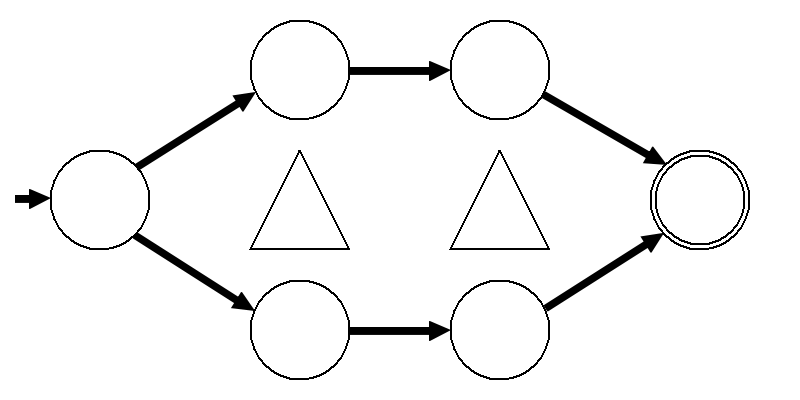
\includegraphics[width=\textwidth-2cm]{images/exanti2.png}
\caption{Exemple d'utilisation d'antichaîne}

\end{center}
\label{dfna}
\end{figure}

Cette illustration représente un automate fini, un cercle est un état, une flèche reliant deux cercles est une transition, l'état initial est celui avec la flèche orpheline pointant vers lui et l'état final est le double cercle.\\

Sur l'exemple en \autoref{dfna}, l'objectif est de savoir s'il existe un chemin d'un état initial à un état final. Nous avons identifié une relation de simulation $\triangleleft$, sur l'image un état avec la pointe du triangle devant lui simule celui qui a la base devant lui. Nous allons exécuter un algorithme de recherche en largeur améliorée. À la première itération, on obtiendra alors les deux états succédant l'initial, on utilisera la fonction $Max$ avec la relation de simulation $\triangleleft$ pour garder celui ou ceux qui ne sont simulés par aucun autre et nous continuerons à utiliser les fonctions $Succ$ et $Max$ jusqu'à stabilité. Dans l'exemple, nous emprunterons donc le chemin du haut jusqu'à l'état final.\\
\end{exem}

\section{Réduction}
Ont été présentés deux problèmes qui semblent différents, de deux domaines différents de l'informatique, pourtant ils peuvent être corrélés. En effet, le but est de résoudre le problème de l'ordonnançabilité à criticité mixte en résolvant celui de l'accessibilité dans un automate. Ces deux problèmes ne sont pas liés tels quels, il va falloir réduire l'un vers l'autre, en l'occurrence, l'ordonnançabilité à criticité mixte vers le l'accessibilité dans un automate.\\

Cette réduction est une passerelle entre deux communautés des sciences informatiques qui n'ont \textit{a priori} pas à se rencontrer.\\

Il s'agit donc de formaliser l'ordonnancement CM en tant que système à transitions étiquetées. La modélisation se basera sur le travail de Baker et Crinei \cite{bakerbrute}, celle-ci formalise toutes les exécutions possibles d'un système de tâches par les différents chemins possibles dans un automate. Cependant, le type d'ordonnancement n'est pas le même. En effet, dans le travail de Baker et Crinei, on retrouve un test d'ordonnançabilité pour un système de tâches sporadiques en multiprocesseur.\\

Certaines notions restent les mêmes, par exemple on se servira d'état du système, nécessitant de savoir pour chaque travail d'une instance le temps avant leur libération $nat$ et le temps restant de calcul $rct$.\\

\begin{defin}[État du système \cite{geeraerts2013multiprocessor}]
Étant donné une instance de $n$ travaux $I = (J_1, ..., J_n)$, l'ensemble des états du système est un ensemble de tuples $S \overset{def}{=} \langle nat_S, rct_S \rangle$
\begin{itemize}
\item $nat_S$ est une fonction de $I$ vers $\mathbb{N}$ tel que pour tout $J_i : nat_S(J_i) \leq O_{max}$ avec $O_{max} \overset{def}{=} max_i\ O_i$
\item $rct_S$ est une fonction de $I$ vers $(1,...,C_{max})$ avec $C_{max} \overset{def}{=} max_i\ C_i$
\end{itemize}
Les états possibles d'une instance $I$ sont représentés par $States(I)$.\\
Ces états semblent infinis, car il n'y a pas de borne inférieure pour $nat$, mais il sera démontré plus tard qu'il y en a bien une.
\end{defin}
Nous remarquons ici que cette définition telle quelle n'est pas adaptée à une système de tâches CM, car elle ne tient pas compte des différents niveaux de criticité, mais elle donne déjà une idée de l'allure qu'elle prendra. Il faudra définir les différents évènements possibles, comme un coup d'horloge ou le passage à une criticité supérieure, tout ceci se retrouvera dans le modèle.



\section{Contribution et structure du mémoire}
Le but de ce mémoire est de trouver un test d'ordonnançabilité CM exact pour un système de tâches CM sporadiques.\\

Dans le \autoref{chap:algoordo}, un éventail des algorithmes d'ordonnancement pour systèmes de tâches CM sporadiques et leur condition suffisante d'ordonnançabilité sera présenté. L'objectif de celui-ci sera double. Premièrement il permettra d'utiliser certains de ces algorithmes dans l'automate explorant les scénarios générés par un système de tâches CM et un algorithme d'ordonnancement. Deuxièmement, il offrira la possibilité de comparer la performance des tests d'ordonnançabilité déjà existants et le test exact créé dans ce mémoire.

Le chapitre évitera de rentrer trop dans les détails, le but est de comprendre comment fonctionnent les différents types d'algorithmes et quel est leur test. C'est pourquoi les preuves seront souvent omises.

Enfin, comme une majorité d'algorithmes ne fonctionnent qu'avec une criticité double, le chapitre se concentre sur cette sous-classe d'algorithme. C'est-à-dire que s'il existe une extension de l'algorithme présenté pour une criticité quelconque, elle ne sera pas présentée.\\

Ensuite viendra le \autoref{chap:automate}, celui-ci offrira la réduction du test d'ordonnançabilité CM vers l'accessibilité dans un automate.

La première section se concentre sur un système de tâches CM périodiques. Cette première réduction permettra de mettre en évidence l'incertitude générée par l'ordonnancement en criticité mixte. De plus, bien que plus restrictives que les tâches CM sporadiques, les tâches CM périodiques restent tout de même intéressantes.

Il s'en suivra la réduction du test d'ordonnançabilité CM pour un système de tâches CM sporadiques vers l'accessibilité dans un automate.

Le chapitre se terminera en présentant une relation de simulation pour l'automate créé à partir d'un système de tâches CM sporadiques. La preuve de l'exactitude de cette relation de simulation formera le cœur de la section.\\

Le pénultième chapitre de ce mémoire, le \autoref{chap:res}, présentera les résultats du travail fourni. Il s'agira, dans un premier temps, de comparer les complexités des solutions aux problèmes de l'ordonnancement CM pour un système de tâches CM périodiques, sporadiques, avec et sans antichaîne. Et, en second lieu, de comparer les tests d'ordonnancement des algorithmes présentés dans le \autoref{chap:algoordo} entre eux, mais aussi avec le nouveau test exact, par exploration d'automate.\\

Enfin, le \autoref{chap:ccl}, exposera les conclusions de ce mémoire, basées sur le chapitre consacré aux résultats. De plus, il proposera différents travaux pour étendre le travail fourni ou pour l'exploiter plus amplement.\\

\chapter{Algorithme d'ordonnancement}
\label{chap:algoordo}

\section{Introduction}
Le but de ce chapitre est de présenter différents algorithmes d'ordonnancement d'un système de tâches CM sporadiques. Cette approche remplit deux objectifs.\\
Premièrement, elle permettra de présenter différentes conditions suffisantes d'ordonnançabilité, autrement dit, des tests d'ordonnancements déjà existants pour ce type d'un système de tâches CM.\\
Ensuite, le modèle qui sera créé dans ce travail vérifiera précisément si un système de tâches CM est ordonnançable avec un certain algorithme. Il faut donc définir cesdits algorithmes.\\

Le chapitre commence par l'introduction de l'algorithme trivial \textit{CAPA}, puis présente ceux basés sur \textit{Audsley} au niveau des tâches CM, ensuite au niveau des travaux CM, enfin, passe en revue ceux basés sur \textit{EDF}, mais modifiant les échéances, pour conclure, un algorithme original \textit{LWLF}.

\section{CAPA}
L'algorithme le plus simple est de définir la priorité des tâches CM en fonction de leur criticité, d'où le nom de cette méthode \textit{Criticality As Priority Assignment, CAPA}. L'idée intuitive de l'algorithme est que l'on souhaite éviter de donner du temps d'accès à la ressource à des tâches CM qui pourraient ne plus être considérées, si un autre ordonnancement avait déclenché une criticité supérieure. Cependant, cet algorithme peut mener à l'échec d'ordonnancement de systèmes de tâches CM même avec une utilisation très faible. Cette faible performance vient de la rigidité de l'assignation des priorités \cite{de2009scheduling}.\\

\pagebreak

\begin{exem}[\cite{santy2012ordonnancement}]
Considérons le système de tâches CM $\tau$ composé de :
\begin{itemize}
\item $\tau_1 = \{0,3,3,1,[1,1]\}$
\item $\tau_2 = \{0,5,5,2,[3,4]\}$
\end{itemize}

L'algorithme \textit{CAPA} assignera statiquement la priorité $\tau_2 \succ \tau_1$, car $\chi_2 > \chi_1$.

\begin{figure}[h]
\centering
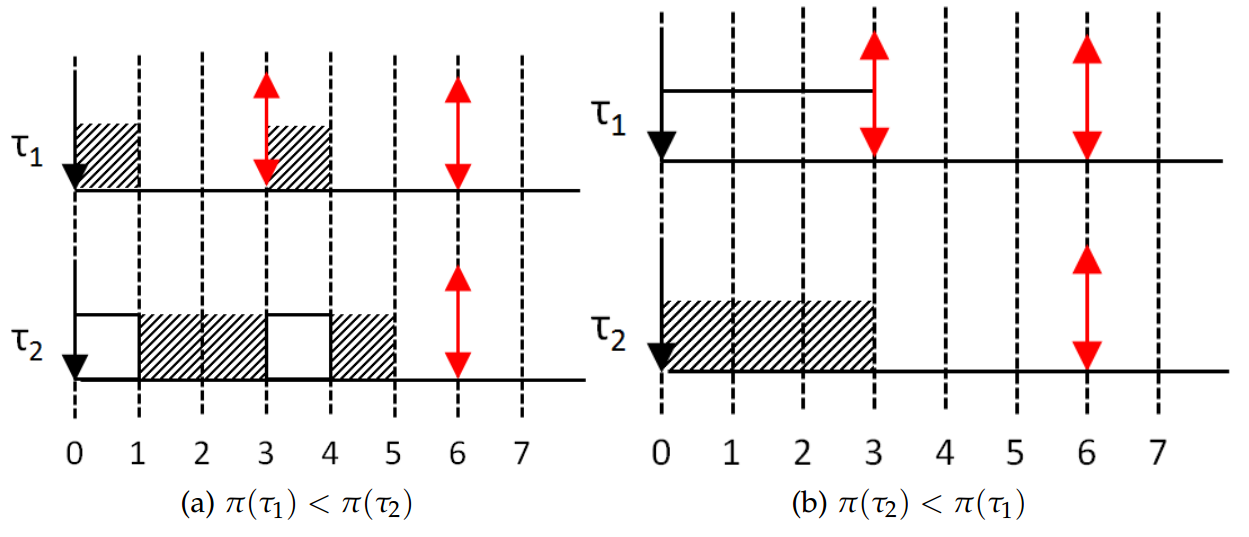
\includegraphics[scale=0.25]{images/capa.png}
\caption{Non optimalité de CAPA \cite{santy2012ordonnancement}}
\label{ordo:capa}
\end{figure}

Dans la \autoref{ordo:capa}, il est apparent que \textit{CAPA} mène à un ordonnancement erroné, alors qu'il est possible d'ordonnancer $\tau$.
\end{exem}

\section{Vestal}
\label{vestal}

\begin{center}
\boxput*(0,1){
\colorbox{white}{Hypothèses}
}{
\setlength{\fboxsep}{6pt}
\fbox {\begin{minipage}{8cm}
\begin{itemize}
\item $K \in \mathbb{N}^*$
\item $D_i \le T_i\ \forall\ i$
\end{itemize}
\end{minipage}}
}
\end{center}

Vestal propose un autre approche \cite{vestal2007preemptive}, basée sur la méthode d'Audsley \cite{audsley1991optimal}. L'algorithme se base sur deux observations, Vestal annonce qu'elles sont maintenues en criticité mixte.

\begin{lem}[\cite{vestal2007preemptive}]
\label{ordo:vestal:low}
Le pire temps de réponse pour une tâche peut être déterminé en sachant quels sous-ensembles de tâches ont une priorité supérieure à elle, mais sans avoir besoin de savoir quelle est l'assignation spécifique de priorité.
\end{lem}

\begin{lem}[\cite{vestal2007preemptive}]
\label{ordo:vestal:higher}
Si une tâche $\tau_i$ est ordonnançable selon une certaine assignation de priorité, elle reste ordonnançable avec une priorité supérieure (les priorités des autres tâches restent identiques).
\end{lem}

L'algorithme commence avec le système de tâches CM sans priorité. Les priorités sont ensuite assignées de la plus faible à la plus forte, de sorte que la première tâche CM assignée sera le plus faiblement prioritaire.\\À chaque étape, l'algorithme sélectionne la tâche CM plus faiblement prioritaire, lui assigne cette priorité et recommence avec l'ensemble des tâches CM sans cette dernière. Si à un moment, aucune tâche CM n'est éligible à recevoir la priorité la plus faible, alors cet algorithme ne permet pas d'ordonnancer ce système de tâches CM.\\

Il est donc nécessaire de déterminer si une tâche CM peut recevoir la plus faible priorité. Pour ce faire, Vestal propose un test basé sur le temps de réponse, faisable par le \autoref{ordo:vestal:low}. \\

\begin{defin}[Pire temps de réponse CM \cite{vestal2007preemptive}]
Le pire temps de réponse CM\index{pire temps de réponse CM} $R_i$ d'une tâche CM $\tau_i$ est la taille maximale de l'intervalle compris entre la génération d'un de ses travaux CM et sa complétion. Le temps de réponse ne peut s'obtenir trivialement. Il s'agit de la somme des WCETs des travaux CM de plus haute priorité que celui de la tâche CM durant l'intervalle $[t, t+R_i)$ où $t$ est l'instant où le travail CM est généré :
\begin{equation}
R_i \overset{def}{=} \underset{\tau_j \in hp(i)}{\sum} \left\lceil\dfrac{R_i}{T_j}\right\rceil C_j(\chi_i)
\end{equation}
Où $hp(i)$ est l'ensemble des tâches CM avec une priorité égale ou  plus élevée que $\tau_i$
\end{defin}

Cette équation récursive peut se résoudre à l'aide d'une itération de point fixe. Il faut commencer par assigner $R_i := C_i(\chi_i)$ et ensuite, évaluer la partie droite de l'équation jusqu'à stabilisation. À tout instant, si $R_i > D_i$ alors la tâche CM ne peut avoir la priorité qui lui a été assignée, sous peine d'un ordonnancement défaillant. Si, lorsque l'itération est terminée, $R_i \leq D_i$ alors $\tau_i$ peut recevoir la priorité la plus faible.

\subsection{AMC-max}

\begin{center}
\boxput*(0,1){
\colorbox{white}{Hypothèses}
}{
\setlength{\fboxsep}{6pt}
\fbox {\begin{minipage}{8cm}
\begin{itemize}
\item $K=2$
\item $D_i \le T_i\ \forall\ i$
\end{itemize}
\end{minipage}}
}
\end{center}
Baruah \textit{et al.} ont étendu les travaux de Vestal et ont trouvé un test pour la viabilité d'une tâche CM à une certaine priorité plus permissif. \cite{baruah2011response}\\
Baruah \textit{et al.} distinguent l'analyse de la viabilité d'une tâche CM à une certaine priorité en trois phases :

\begin{itemize}
\item Vérifier l'ordonnançabilité en criticité $LO$
\item Vérifier l'ordonnançabilité en criticité $HI$
\item Vérifier l'ordonnançabilité du changement de criticité
\end{itemize}
Pour effectuer ces tests, une extension du pire temps de réponse CM est faite, prenant en compte la criticité.\\

\begin{defin}[Pire temps de réponse CM en criticité $\ell$ \cite{baruah2011response}]
Le pire temps de réponse CM\index{pire temps de réponse CM} $R_i^\ell$ d'une tâche CM $\tau_i$ au niveau $\ell$ est la taille maximale de l'intervalle compris entre la génération d'un de ses travaux CM et sa complétion lorsque ce travail CM est généré quand la criticité est $\ell$. Il s'agit de la somme des WCETs au niveau $\ell$ des tâches CM toujours présentes et de plus haute priorité que celle de la tâche CM durant l'intervalle $[t, t+R_i^\ell)$ où $t$ est l'instant où le travail CM est généré, et de $C_i(\chi_i)$, le pire temps d'exécution de $\tau_i$ :

\begin{equation}
R_i^\ell \overset{def}{=} C_i(\chi_i) +\underset{\tau_j \in hp(i, \ell)}{\sum} \left\lceil\dfrac{R_i^\ell}{T_j}\right\rceil C_j(\ell)
\end{equation}

Où $hp(i, \ell)$ est l'ensemble des tâches CM de criticité au moins $\ell$, avec une priorité plus élevée que $\tau_i$
\end{defin}

Pour vérifier l'ordonnançabilité en criticité $LO$ et $HI$, on utilise les tests standards : $R_i^{LO} \le D_i \wedge R_i^{HI} \le D_i$. Ici $R_i^\ell$ est assigné à zéro pour la première itération.\\

Le pire temps de réponse CM d'une tâche CM $\tau_i$ lors d'un changement de criticité est noté $R_i^*$. Pour le trouver, on définit l'interférence maximale d'une tâche CM hautement critique s’il y a un changement de criticité, généré par une tâche CM $\tau_s$ à un instant $s$. Le passage au niveau de criticité supérieur est déclenché lorsqu'une tâche CM $\tau_s$ s'exécute pour plus longtemps que $C_s(LO)$. Si cet évènement impacte $\tau_i$, cela signifie que $s < R^{LO}_i$, et la priorité de $\tau_s$ est supérieure ou égale à celle de $\tau_i$; sinon $\tau_i$ se serait complétée avant le changement de criticité. On crée alors $R^s_i$, le pire temps de réponse de la tâche CM $\tau_i$, lorsqu'un changement de criticité se passe au temps $s$, relativement au temps de génération de $\tau_i$.

\begin{equation}
R_i^s \overset{def}{=} C_i(HI) + I_L(s) + I_H(s)
\end{equation}

où $I_L(s)$ est l'interférence venant des tâches CM avec une criticité plus faible que $\tau_i$ et $I_H(s)$ est l'interférence venant des tâches CM avec une criticité supérieure ou égale à celle de $\tau_i$.\\

\pagebreak

Les tâches CM de criticité plus faible sont abandonnées après $s$ et donc leur interférence est bornée par :

\begin{equation}
I_L(s) \overset{def}{=} \underset{j \in hp(i) \wedge \chi_j = LO}{\sum} (\left\lfloor \dfrac{s}{T_j} \right\rfloor + 1) C_j(LO)
\end{equation}

La valeur $plancher +1$ est utilisée, car dès qu'un travail CM est émise, il faut considérer son interférence. Attention, ici on n'utilise pas $hp(i, LO)$, car on souhaite ne considérer que les tâches CM de basse criticité.\\

Pour l'interférence $I_H(s)$, on supposera que tous les travaux CM actifs au temps $s$, s'exécutent pour $C(HI)$ unité de temps. D'où, seuls les travaux CM avec une échéance avant $s$ utilisent leurs estimations pour la criticité $LO$.\\

Considérons l'interférence d'une tâche CM $\tau_k$ au temps $t$ avec $t > s$. Le nombre maximum d'émissions que la tâche CM peut faire est $\lceil t / T_k \rceil$. Le nombre maximum d'émissions qu'une tâche CM peut faire durant l'intervalle $t$ - $s$ est borné par 

\begin{equation}
\label{amc:nbrel:pess}
\left\lceil \dfrac{t-s-(T_k-D_k)}{T_k} \right\rceil +1
\end{equation}

Cependant, si $s$ est petit et $D_k$ trop proche de $T_k$ alors l'\autoref{amc:nbrel:pess} peut inclure plus de travaux CM qu'il n'y en a vraiment. On définit donc

\begin{equation}
M(k,s,t) = min \left\lbrace \left\lceil \dfrac{t-s-(T_k-D_k)}{T_k} \right\rceil +1, \left\lceil \dfrac{t}{T_k} \right\rceil \right\rbrace
\end{equation}

L'interférence au temps $t$ est alors

\begin{equation}
I_H(s) \overset{def}{=} \underset{k \in hp(i, HI)}{\sum} \left( M(k,s,t)C_k(HI) + \left(\left\lceil \dfrac{t}{T_k} \right\rceil - M(k,s,t)\right) C_k(LO) \right)
\end{equation}

Et donc 

\begin{equation}
R_i^s = C_i(HI) + \left( \underset{j \in hp(i) \wedge \chi_j = LO}{\sum} (\left\lfloor \dfrac{s}{T_j} \right\rfloor + 1) C_j(LO) \right) +$$\\$$\underset{k \in hp(i, HI)}{\sum} \left( M(k,s,R_i^s)C_k(HI) + \left(\left\lceil \dfrac{R_i^s}{T_k} \right\rceil - M(k,s,R_i^s)\right) C_k(LO) \right)
\end{equation}

\pagebreak

Avec

\begin{equation}
R_i^* \overset{def}{=} max(R_i^s) \forall s
\end{equation}

Il reste à trouver quelles sont les $s$ à tester. L'intervalle possible pour $s$ va de $0$ à $R^{LO}_i$. En analysant $R_i^s$, il faut remarquer que le terme avec $j \in hp(i) \wedge \chi_j = LO$ augmente avec $s$, alors que le terme avec $hp(i, HI)$ diminue avec $s$. D'où, $R_i^s$ ne peut augmenter que lorsqu'une tâche CM faiblement critique génère un travail CM, il s'agit donc des points à prendre en compte.

\section{OCBP}
\label{ocbpext}
\begin{center}
\boxput*(0,1){
\colorbox{white}{Hypothèses}
}{
\setlength{\fboxsep}{6pt}
\fbox {\begin{minipage}{8cm}
\begin{itemize}
\item $K = 2$
\item $D_i \in \mathbb{N}^*\ \forall\ i$
\end{itemize}
\end{minipage}}
}
\end{center}

\textit{OCBP} est un algorithme d'ordonnancement basé sur assignation de priorités. Dans la même veine que \textit{Vestal} et \textit{AMC-max}, cet ordonnanceur cherche à assigner la priorité la plus basse récursivement. Cependant, ici ce sont directement les travaux CM qui sont considérés et non les tâches CM. L'algorithme se base uniquement sur le WCET de la criticité d'une tâche CM pour son assignation, c'est pour ça qu'il s'appelle \textit{Own Criticality Based Priority, OCBP}.\\

Une première version de cet algorithme a été imaginée pour une instance de travaux CM, dans cette configuration, l'assignation de priorité se fait hors ligne \cite{baruah2010towards}. Il semble alors évident de simplement appliquer cette version de l'algorithme pour l'instance CM de travaux CM générée par un système de tâches CM sporadiques. Cependant, cette approche est impossible. Premièrement, la phase hors-ligne d'assignation des priorités peut être infinie, puisque l'instance de travaux CM générés par le système de tâches CM sporadiques est potentiellement infinie. Ensuite, et surtout, l'algorithme dans sa version sur instance CM requiert d'avoir une spécification précise des travaux CM. Or avec des tâches CM sporadiques, il n'est pas possible de savoir exactement quand les travaux CM seront générés, seule une borne inférieure est disponible.\\

La suite de cette section présente l'algorithme \textit{OBCP} pour des tâches CM sporadiques présenté dans l'ouvrage \cite{li2010algorithm}, mais ne s'attarde pas sur la résolution de ces problèmes énoncés. Pour les découvrir, consultez ce même ouvrage.\\

L'algorithme fait appel à la notion de période occupée, elle-même basée sur celle d'instant oisif, ci-dessous leur définition.\\

\begin{defin}[Instant oisif \cite{goossens1999scheduling}]
$x \in \mathbb{N}$ est un instant oisif\index{instant oisif} de l'ordonnancement d'un système si toutes les requêtes émises strictement avant $x$ ont été complétées, avant ou au temps $x$.\\
\end{defin}

\begin{defin}[Période occupée \cite{goossens1999scheduling}]
Une période occupée\index{période occupée} est un intervalle $[a, b)$, tel que $a$ et $b$ sont deux instants oisifs, le processeur est occupé durant l'intervalle et il n'y a pas d'instant oisif intermédiaire. 
\end{defin}

Supposons qu'une période occupée commence à un instant $t_0$, durant l'exécution. À cet instant, il faut assigner une priorité à tous les travaux CM qui pourraient potentiellement arriver dans la période occupée commençant à $t_0$, comme si tous les travaux CM étaient émis au premier instant permis. Pour le bon fonctionnement de l'algorithme \textit{OCBP}, il faut considérer que tous ces travaux CM sont \textit{générés-au-plus-tôt}\index{généré-au-plus-tôt}. Ce principe est illustré avec l'\autoref{ocbp:exem:ordo}.\\

\begin{exem}
\label{ocbp:exem:ordo}
Supposons qu'une tâche CM $\tau_i$ peut générer trois travaux CM durant la période occupée commençant à $t_0$. Au plus tôt, ces travaux CM seront générés au temps $t_0, t_0+T_i, t_0+2*T_i$ respectivement et auront pour échéance $t_0+D_i, t_0+T_i+D_i, t_0+2*T_i+D_i$ respectivement. Considérer ces travaux CM comme \textit{générés-au-plus-tôt} signifie que leur temps d'arrivée sera $t_0$ pour chacun d'entre eux, leurs échéances restent inchangées.\\

Formellement, $\{J_i\}^n_{i=1}$ dénote tous ces travaux CM à $t_0$; $J_i = (t_0, d_i, \chi_i, c_i)$
\end{exem}

\subsection{Assignation des priorités}
Il faut assigner les priorités aux travaux CM $\{J_i\}^n_{i=1}$ conformément à l'assignation de priorité \textit{OCBP}. Cette assignation de priorité est la fonction $\pi : \{J_i\}^n_{i=1} \rightarrow {1,2,...,n}$.\\

L'assignation \textit{OCBP} fonctionne de la manière suivante :\\

Déterminer au sein d'une instance CM $I$, le travail CM $J_i$ le plus faiblement prioritaire : un travail CM $J_i$ peut avoir la priorité la plus faible si

\begin{itemize}
\item c'est un travail CM faiblement critique ($\chi_i = LO$), et il y a au moins $c_i(LO)$ temps entre son émission et son échéance, si tous les autres travaux CM $J_j$ ont une priorité plus élevée et sont exécutés pour $c_j(LO)$ unité de temps; ou
\item c'est un travail CM fortement critique ($\chi_i = HI$), et il y a au moins $c_i(HI)$ temps entre son émission et son échéance, si tous les autres travaux CM $J_j$ ont une priorité plus élevée et sont exécutés pour $c_j(HI)$ unité de temps.
\end{itemize}

En général, il est possible que plusieurs travaux CM soient éligibles pour être le travail CM le plus faiblement prioritaire, il faut alors en choisir arbitrairement un. Cette procédure est répétée pour l'ensemble des travaux CM; sans ce travail CM avec une priorité récemment assignée, jusqu'à ce que tous les travaux CM aient une priorité assignée ou que le travail CM le plus faiblement prioritaire ne puisse être trouvé. Dans ce dernier cas, l'instance CM $I$ n'est pas ordonnançable avec \textit{OCBP} et donc le système de tâches CM $\tau$ non plus.

\subsection{Ordonnancement durant l'exécution}
Durant l'exécution, à tout moment, le travail CM $J_i$ qui a été généré, mais pas encore signalé comme complété avec la valeur $\pi(J_i)$ la plus faible, est sélectionné pour exécution. Ce procédé continue jusqu'à ce que l'un des évènements suivants arrive :

\paragraph{E-1}
Un travail CM $J_i$ s'exécute pour plus que $c_i(LO)$ unité de temps sans signaler sa complétion. Ceci implique que le système est maintenant de criticité $HI$ et que les travaux CM de criticité $LO$ ne doivent plus être complétés d'ici leurs échéances. Il s'en suit, selon l'exactitude de l'assignation de priorité \textit{OCBP} à $t_0$, que les travaux CM de criticité $HI$ qui arriveront durant la période occupée courante sont garantis d'être exécutés jusqu'à leur complétion.

\paragraph{E-2}
Selon \textit{OCBP}, le processeur est oisif à un certain instant $t$, seulement si tous les travaux CM qui ont été générés avant $t$ se sont complétés avant ou au temps $t$. Si c'est le cas, la période occupée courante est terminée et les priorités qui ont été assignées aux travaux CM qui n'ont pas été émis sont annulées. Il faut alors attendre la prochaine émission d'un travail CM, qui va signaler le début d'une nouvelle période occupée. À ce moment-là, il faut recalculer les priorités de tous les travaux CM qui pourraient arriver durant cette nouvelle période occupée.

\paragraph{E-3}
L'exécution d'un travail CM $J_x$ moins prioritaire est préemptée à cause de la génération d'un travail CM de plus haute priorité $J_y$ ($\pi(J_y) < \pi(J_x)$), à l'instant $t_1$. Il faut alors recalculer la fonction de priorité $\pi$ à ce moment précis. Les travaux CM ayant une priorité plus faible que celle de $J_x$ garderont leur priorité actuelle.\\

Réassignation des priorités : pour tout $i$, soit $\Delta_i$ le nombre de temps d'exécution, dont le travail CM $J_i$ a bénéficié durant l'intervalle $[t_0, t_1)$. Soit $c_i'(LO) \overset{def}{=} c_i(LO)-\Delta_i$, $c_i'(HI) \overset{def}{=} c_i(HI)-\Delta_i$ et $c_i' \overset{def}{=} [c_i'(LO), c_i'(HI)]$; ceux-ci dénotent les WCETs restants pour $J_i$.\\

Il est possible de considérer la charge de travail restante à exécuter durant la période occupée comme l'instance 

\begin{equation}
\left\lbrace J_i' = (t_1, d_i, \chi_i, c'_i) \right\rbrace^n_{i=1}
\end{equation}

Supposons que $(n-n')$ travaux CM ont signalé leurs complétions, durant $[t_0, t_1)$ : ce sont les travaux CM $J_k$ avec $\pi(J_k) < \pi(J_x)$, car sinon, $J_x$ aurait été exécuté avant eux.\\
Soit $\{J_i'\}^{n'}_{i=1}$ les travaux CM restants. L'assignation de priorité

\begin{center}
$\pi' : \{J_i'\}^{n'}_{i=1} \rightarrow {1,2,...n'}$
\end{center}

est obtenue depuis $\pi$ comme suit :

\begin{enumerate}
\item Tous les travaux CM $J_k$ satisfaisant $\pi(J_k) < \pi(J_x)$, qui n'ont pas encore complété leur exécution, ont les priorités $\pi'(J_k)$ recalculées par \textit{OCBP} sous l'hypothèse de \textit{génération-au-plus-tôt}, qu'ils sont tous générés à l'instant $t_1$
\item Pour tous les travaux CM $J_k$ satisfaisants $\pi(J_k) \geq \pi(J_x), \pi'(J_k) \leftarrow \pi(J_k) -(n-n')$
\end{enumerate}

L'algorithme est totalement présenté.

\subsection{Test d'ordonnancement}
Il existe une condition suffisante d'ordonnançabilité pour \textit{OCBP} venant de l'article \cite{guan2011effective}, cette sous-section la présente.\\

Le test d'ordonnancement se base sur la charge de travail\index{charge de travail}. Dans l'ordonnancement temps réel classique, il s'agit du maximum, sur tous les intervalles possibles, du temps d'exécution requis cumulé par le système de tâches CM, normalisé par l'intervalle \cite{guan2011effective}. Il s'agit donc d'une borne inférieure sur la portion de la capacité d'exécution requise par le système de tâches CM pour respecter toutes les échéances.\\

Parallèlement à ce concept, il est possible de définir la charge de travail pour un système de tâches CM à chaque niveau de criticité.\\

\begin{defin}[Charge $\ell$-critique]
La charge $\ell$-critique\index{charge $\ell$-critique} d'un système de tâches CM $\tau$ est définie par 

\begin{center}
$\Gamma_\ell(\tau) \overset{def}{=} \underset{0\leq t_1 \leq t_2}{max} \left\lbrace \underset{\forall J_i:\chi_i \geq \ell \wedge t_1 \leq r_i\wedge d_i\leq t_2}{\sum} c_i(\ell)/(t_2-t_1) \right\rbrace$
\end{center}
\end{defin}

Pour toute criticité $\ell$, $\Gamma_\ell(\tau)$ peut être calculée avec des techniques pour déterminer les charges de travail d'un système de tâches traditionnelles \cite{Baker05algorithmsfor}.\\Intuitivement, $\Gamma_\ell(\tau)$ représente une borne inférieure sur la portion de capacité d'exécution requise par ce système de tâches CM, avec laquelle elle peut respecter toutes ses échéances sujettes seulement à la certification au niveau de criticité $\ell$. Pour exécuter correctement un système de tâches CM sporadiques, une condition nécessaire est que cette portion de capacité d'exécution requise ne dépasse pas 1 (avec un processeur à vitesse unitaire).\\

Dans cette section, \textit{OCBP} est présenté dans le contexte d'un système à criticité double uniquement. Cependant, cet algorithme peut être étendu pour gérer un système de tâches CM sporadiques avec plus de deux niveaux de criticité. Il est alors possible d'utiliser les connaissances venant de \cite{baruah2010mixed} pour obtenir le test d'ordonnancement CM suivant :

\begin{equation}
\label{test:ocbp}
\forall \ell \in [1,K] : \Gamma_\ell(\tau) \le LoadBound(K)
\end{equation}

Où $\Gamma_\ell(\tau)$ est la charge au niveau de criticité $\ell$, et $LoadBound(K)$ est une fonction avec respect du nombre total de niveau criticité $K$ du système, qui est calculée récursivement :

\begin{center}
$LoadBound(1) = 1$\\
$LoadBound(K) = \dfrac{2}{1+\sqrt{4\dfrac{1}{LoadBound(K-1)^2}+1}}$
\end{center}

Pour le cas spécial où $K = 2$, une condition sur la charge plus précise est disponible \cite{li2010load} :

\begin{equation}
(\Gamma_{HI}(\tau))^2+\Gamma_{LO}(\tau) \le 1
\end{equation}

Voilà qui offre un test d'ordonnançabilité pour \textit{OCBP}.

\subsection{Taille de la plus grande période occupée}
Lors de l'ordonnancement, il est nécessaire de connaître la taille de la plus grande période occupée pour assigner les priorités aux travaux CM qui y figurent. À nouveau, l'article \cite{baruah2010towards} propose une borne supérieure pour celle-ci.\\

La taille de la plus grande période occupée est divisée en deux. Premièrement, $x_1$ est l'intervalle commençant au début de la plus grande période occupée jusqu'au moment où un travail CM dépasse son WCET de criticité $LO$, s'il y en a un. Ensuite, $x_2$ est l'intervalle qui commence à la fin de $x_1$ et se termine à la fin de la plus grande période occupée.\\

Soit $D_{max} \overset{def}{=} max_i D_i$. Tous les travaux CM exécutés pendant $[0, x_1)$ ont leur temps de génération et leur échéance durant l'intervalle $[0, x_1+D_{max}]$, d'où
\begin{equation}
x_1 \le \Gamma_{LO}(\tau)(D_{max}+x_1)$$
$$x_1(1-\Gamma_{LO}(\tau))\le \Gamma_{LO} \times D_{max}$$
$$x_1 \le \dfrac{\Gamma_{LO}(\tau)}{1-\Gamma_{LO}(\tau)} \times D_{max}
\end{equation}

Vu que tous les travaux CM exécutés durant $[x_1, x_1+x_2)$ ont leur temps de génération et leur échéance durant l'intervalle $[x_1, x_1+x_2+D_{max}]$, on en déduit que

\begin{equation}
x_2 \le \Gamma_{HI}(\tau)(D_{max} + x_1+x_2) $$
$$x_2(1-\Gamma_{HI}(\tau)) \le \Gamma_{HI}(\tau)\times(D_{max}+x_1)$$\
$$x_2 \le \dfrac{\Gamma_{HI}(\tau)}{1-\Gamma_{HI}(\tau)} \times (D_{max} +x_1)$$\
$$x_2 \le \dfrac{\Gamma_{HI}(\tau)}{1-\Gamma_{HI}(\tau)} \times (D_{max} + \dfrac{\Gamma_{LO}(\tau)}{1-\Gamma_{LO}(\tau)} \times D_{max})$$
$$x_2 \le \dfrac{\Gamma_{HI}(\tau)}{(1-\Gamma_{HI}(\tau))(1-\Gamma_{LO}(\tau))} \times D_{max}
\end{equation}

La taille de la plus grande période occupée est donc plafonnée par $x_1+x_2$. Une fois que la plus grande période occupée est bornée, il facile d'obtenir les travaux CM qui peuvent s'y générer.

\section{PLRS et LPA}

\label{plrslpa}

\begin{center}
\boxput*(0,1){
\colorbox{white}{Hypothèses}
}{
\setlength{\fboxsep}{6pt}
\fbox {\begin{minipage}{8cm}
\begin{itemize}
\item $K \in \mathbb{N}^*$
\item $D_i \in \mathbb{N}^*\ \forall\ i$
\end{itemize}
\end{minipage}}
}
\end{center}

\textit{PLRS}, \textit{Priority List Reuse Scheduling} est une extension d'\textit{OCBP}, mais considère les instants où un travail CM plus prioritaire que celui exécuté actuellement est généré de manière plus abstraite, pour alléger le temps de calcul. \textit{LPA}, \textit{Lazy Priority Adjustment} est une extension de \textit{PLRS}, qui utilise notamment une taille maximale de période occupée plus restreinte. Ces deux algorithmes étant fort proches de l'initial, cette sous-section ne fera que présenter leur condition suffisante d'ordonnancement.

\pagebreak

\paragraph{PLRS} commence par faire une assignation de priorité initiale et la modifiera en ligne. S'il est possible de faire cette assignation pour un système de tâches CM, il est ordonnançable CM avec \textit{PLRS} \cite{guan2011effective}. Cette assignation est en fait la même que celle pour \textit{OCBP}. Guan \textit{et al.} proposent d'utiliser cette formulation : chaque tâche CM $\tau_k$ a un nombre $\delta_k$ représentant le nombre de travaux CM qu'elle générera durant la période occupée au maximum, qui n'ont pas encore de priorité assignée. Initialement, $\delta_k$ vaut donc le nombre de travaux CM que la tâche CM $\tau_k$ générera durant la période occupée au maximum. L'algorithme commence par décider quel travail CM ayant l'index le plus élevé peut recevoir la priorité la plus faible. Le travail CM $J^{\delta_k}_k$ est éligible à recevoir la priorité la plus faible si

\begin{equation}
\underset{\tau_j \in \tau}{\sum} (\delta_j \times C_j(\chi_k)) \le (\delta_k-1) \times T_k + D_k
\end{equation}

La partie gauche de l'inéquation représente la charge de travail restante des travaux CM présents dans l'instance CM composée des travaux CM générés par les tâches CM présentes dans $\tau$ durant la période occupée maximale, si le système est de criticité $\chi_k$. La partie de droite de l'inéquation est la distance minimale entre l'échéance absolue de $J^{\delta_k}_k$ et le début la période occupée considérée. Si plusieurs travaux CM peuvent recevoir la priorité la plus faible, il faut en choisir un arbitrairement. Une fois ce travail CM le plus faiblement prioritaire désigné, il faut décrémenter $\delta_k$ d'une unité pour exclure ce travail CM lors des prochaines étapes. La période occupée maximale est la même que celle dans \textit{OCBP}.\\

Par la suite, l'algorithme itère jusqu'à ce que tous les travaux CM aient une priorité. Si ce n'est pas possible, alors le système de tâches CM n'est pas ordonnançable avec \textit{PLRS}. Attention, bien que si un système de tâches CM passe cette assignation signifie qu'il est ordonnançable avec \textit{PLRS}, suivre ses priorités en tant que telles ne fonctionnera pas forcément. En effet, l'algorithme modifiera les priorités en ligne, cette partie est consultable en \cite{guan2011effective}.

\paragraph{LPA}, en fidèle successeur d'\textit{OCBP}, commence par faire une assignation de priorité hors ligne. Il s'agit de la même que \textit{PLRS}. À nouveau, si un système de tâches CM passe cette assignation, alors il est ordonnançable avec \textit{LPA} \cite{gu2013improving}. Ici, Gu \textit{et al.} proposent une nouvelle façon de calculer la taille de la période maximale.\\

Gu \textit{et al.} définissent la charge $\ell$-critique\index{charge $\ell$-critique} comme la borne supérieure de la charge totale des tâches CM dont la criticité n'est pas supérieure à $\ell$, dans toutes les périodes occupées, où la criticité ne dépasse pas $\ell$. D'où $\Gamma_K(\tau)$ est la borne supérieure pour la taille des périodes occupées pour le système de tâches CM $\tau$. Et ils posent $\Gamma_0(\tau) = 0$.\\
Ensuite, ils prouvent le théorème suivant.\\

\begin{theo}[\cite{gu2013improving}]
Étant donné un système de tâches CM sporadiques $\tau$ et la charge $\ell-1$-critique $\Gamma_{\ell-1}$, on a:
\begin{equation}
\phi_\ell = \dfrac{\Gamma_{\ell-1}(\tau) + \sum_{\chi_i \ge \ell} C_i(\ell)}{1 - \sum_{\chi_i \ge \ell} \dfrac{C_i(\ell)}{T_i}}
\end{equation}
\begin{equation}
\Gamma_\ell(\tau) = \Gamma_{\ell-1}(\tau) + \underset{\chi_i = \ell}{\sum}C_i(\ell) \times \left( 1 + \left\lfloor \dfrac{\phi_\ell}{T_i} \right\rfloor \right)
\end{equation}
\end{theo}

Depuis ce théorème, Gu \textit{et al.} proposent l'algorithme suivant pour calculer la charge et ensuite réutilisent la manière de créer la période occupée d'\textit{OCBP}, en utilisant leur nouvelle façon de calculer la charge.

\begin{algorithm}[caption={Calcul de la charge $\ell$-critique},label={lpalgo},mathescape=true]
ComputeGamma($\ell$)
 if $\ell = 0$ then
  return 0
 endif
 $\displaystyle \Gamma_\ell(\tau) \gets $ComputeGamma($\ell-1$)
 $\displaystyle \gamma_\ell \gets \dfrac{\Gamma_\ell(\tau) + \sum_{\chi_i \geq \ell} C_i(\ell)}{1-\sum_{\chi_i \geq \ell} \dfrac{C_i(\ell)}{T_i}}$
 
 return $\displaystyle \Gamma_{\ell-1}(\tau) + \sum_{\chi_i = \ell}C_i(\ell) \times \left( 1 + \left\lfloor \dfrac{\gamma_\ell}{T_i} \right\rfloor \right)$
       
\end{algorithm}
\phantom\\
 Avec l'\autoref{lpalgo}, on peut obtenir $\Gamma_K(\tau)$, il s'agit de ComputeGamme($K$).\\

\section{EDF-VD}
\label{edfvd}

\begin{center}
\boxput*(0,1){
\colorbox{white}{Hypothèses}
}{
\setlength{\fboxsep}{6pt}
\fbox {\begin{minipage}{8cm}
\begin{itemize}
\item $K = 2$
\item $D_i = T_i\ \forall\ i$
\end{itemize}
\end{minipage}}
}
\end{center}

Baruah \textit{et al.} proposent un algorithme\cite{BaruahBDMSS11} qui est une variante de \textit{EDF}, appelé \textit{EDF} à échéance virtuelle, \textit{EDF-VD}, pour \textit{Virtual Deadlines}.
Pour la compréhension de l'algorithme, l'explication qui suit considère un système de tâches CM avec une criticité double.\\

Il faut distinguer deux cas :

\begin{itemize}
\item Cas 1. $U_1(1) + U_2(2) \le 1$ : appliquer \textit{EDF} avec les échéances des tâches CM non modifiées. Dès que le système passe au niveau 2, abandonner les tâches CM de niveau 1.
\item Cas 2. $U_1(1) + \dfrac{U_2(1)}{1-U_2(2)} \le 1$ et le cas 1 n'est pas satisfait : $\lambda = \dfrac{U_2(1)}{1-U_1(1)}$. Lorsque le système est en criticité 1 : pour toutes tâches CM $\tau_i$ avec $\chi_i = 2, \widehat{p}_i \overset{def}{=} \lambda p_i$. Redéfinir les échéances des tâches CM telles que $\chi_i = 2$ en y ajoutant $\widehat{p}_i$ au temps des générations de chacun de leurs travaux. Ne pas modifier les échéances des tâches CM avec $\chi _i =1$ et appliquer \textit{EDF}. Lorsque le système atteint la criticité de niveau 2, abandonner les tâches CM de criticité de niveau 1 et réinitialiser les échéances des tâches CM encore considérées et appliquer \textit{EDF} sur ces échéances initiales.
\end{itemize}

Baruah \textit{et al.} donnent ensuite une condition suffisante d'ordonnançabilité :\\

\begin{theo}[\cite{BaruahBDMSS11}]
Si $\tau$ satisfait
\begin{center}
$U_1(1) + min \left( U_2(2), \dfrac{U_2(1)}{1-U_2(2)} \right) \le 1$
\end{center}
Alors $\tau$ est ordonnançable avec \textit{EDF-VD}.\\
\end{theo}

\phantom{Bien que Baruah \textit{et al.} définissent cette condition suffisante d'ordonnançabilité pour des tâches CM à échéance implicite, elle reste pertinente pour des échéances contraintes \cite{ekberg2012outstanding}.}\phantom\\

\textit{EDF-VD} a été généralisé pour des systèmes de tâches CM avec un niveau de criticité plus élevé que $2$, l'extension est consultable dans l'ouvrage \cite{BaruahBDMSS11}.

\section{Greedy}
\begin{center}
\boxput*(0,1){
\colorbox{white}{Hypothèses}
}{
\setlength{\fboxsep}{6pt}
\fbox {\begin{minipage}{8cm}
\begin{itemize}
\item $K = 2$
\item $D_i \leq T_i\ \forall\ i$
\end{itemize}
\end{minipage}}
}

\end{center}
Ekberg \textit{et al.} ont proposé un algorithme sur l'analyse de la demande des tâches CM \cite{ekberg2012outstanding}, cette section le présente.\\

\pagebreak

Une approche connue pour l'analyse de l'ordonnancement en temps réel classique est d'utiliser une fonction de borne de demande \cite{baruah1990preemptively}. Une fonction de borne de demande capture la demande d'exécution maximale d'une tâche durant un intervalle d'une taille donnée.\\

\begin{defin}[Fonction de borne de demande \cite{ekberg2012outstanding}]
Une fonction de borne de demande\index{fonction de borne de demande} $dbf(\tau_i, \Delta)$ donne une borne supérieure pour la demande d'exécution maximale possible d'une tâche $\tau_i$ dans tous les intervalles de temps d'une taille $\Delta$, où la demande est calculée comme le temps d'exécution requis total des travaux avec leur fenêtre d'ordonnancement ($[r_i, d_i)$) complètement dans l'intervalle.
\end{defin}

Un concept similaire est la fonction de borne d'approvisionnement\index{fonction de borne d'approvisionnement} $sbf(\Delta)$ qui limite inférieurement la quantité de temps d'exécution fournie par le processeur dans tous les intervalles de taille $\Delta$. Par exemple, sur un processeur à vitesse unitaire, $sbf(\Delta) = \Delta$.\\

Ce qui rend les fonctions de borne de demande et d'approvisionnement intéressantes, c'est la proposition suivante :

\begin{prop}
\label{greedy:class:dbfsbf}
Un système de tâches $\tau$ (sans criticité mixte) est ordonnançable par \textit{EDF} sur monoprocesseur avec la fonction de borne inférieure $sbf$ si :
\begin{center}
$ \forall \Delta \ge 0 : \underset{\tau_i \in \tau}{\sum}dbf(\tau_i, \Delta) \le sbf(\Delta)$
\end{center}
\end{prop}

Ekberg \textit{et al.} étendent l'idée de la fonction de borne de demande à la criticité mixte, avec double criticité. Pour toute tâche CM, ils construisent deux fonctions de borne de demande, $dbf_{LO}$ et $dbf_{HI}$, pour les modes de criticité bas et haut respectivement. La \autoref{greedy:class:dbfsbf} est étendue :

\begin{prop}
\label{greedy:mc:dbfsbf}
Un système de tâches CM sporadiques $\tau$ est ordonnançable par \textit{EDF} sur un processeur avec la fonction de borne inférieure $sbf_{LO}$ dans le mode à criticité basse et $sbf_{HI}$ dans le mode à criticité haute si les deux conditions suivantes sont satisfaites :
\begin{center}
\textbf{\textit{Condition A:}}$\quad \forall \Delta \ge 0 : \underset{\tau_i \in \tau}{\sum}dbf_{LO}(\tau_i, \Delta) \le sbf_{LO}(\Delta)$\\
\textbf{\textit{Condition B:}}$\quad \forall \Delta \ge 0 : \underset{\tau_i \in \tau}{\sum}dbf_{HI}(\tau_i, \Delta) \le sbf_{HI}(\Delta)$
\end{center}
\end{prop}

Les conditions A et B s'assurent de l'ordonnançabilité du système de tâches CM en basse et haute criticité. Bien que ces deux modes puissent être analysés séparément avec les conditions ci-dessus, la demande en haute criticité dépend de ce qui se passe en basse criticité.\\

Pour trouver ces fonctions de borne de demande, on suppose, sans perte de généralité, que $sbf_{LO}$ est de vitesse unitaire au maximum.\\

Dans le cas de la criticité basse, l'exercice est simple. Dans ce mode, les tâches CM $\tau_i$ se comportent comme des tâches sporadiques normales, et tous leurs travaux CM finissent, au pire, après $C_i(LO)$ unités de temps. Il est donc possible d'utiliser des méthodes standards pour calculer les fonctions de borne de demande pour tâches sporadiques \cite{baruah1990preemptively}.\\

Avec $dbf_{HI}$, c'est plus compliqué, car il faut considérer les travaux CM de criticité haute qui ont été actifs durant le changement de criticité.\\

\begin{defin}[Travaux transférés \cite{ekberg2012outstanding}]
Un travail CM émis par une tâche CM à haute criticité  qui est actif (généré, mais non terminé) au moment du changement de criticité est appelé un travail transféré\index{travail transféré}.
\end{defin}

\subsection{Analyse de la demande des travaux transférés}
En haute criticité, il faut finir l'exécution restante des travaux transférés avant leur échéance. La demande de ces travaux transférés doit donc être prise en considération dans chaque $dbf_{HI}$ des tâches CM de haute criticité. Conceptuellement, lors de l'analyse de l'ordonnançabilité en haute criticité, on peut considérer les travaux transférés comme des travaux CM ayant été générés lors du changement de criticité. Cependant, la fenêtre d'ordonnancement devient l'intervalle entre le changement de criticité et l'échéance du travail CM, et peut donc être plus courte que d'autres travaux CM générés par la même tâche CM. Parce que ces travaux CM ont pu déjà être exécutés pour quelques unités de temps, le temps restant de calcul peut être inférieur à celui des autres travaux CM générés par la même tâche CM.\\

Pour borner la demande en haute criticité (condition B), on suppose que la demande en basse criticité est approvisionnée, sinon le système de tâches CM ne peut être ordonnançable. Il s'agit donc de démontrer $A \wedge (A \rightarrow B)$, ce qui permettra d'affirmer $A\wedge B$.\\

Analysons les informations disponibles sur les travaux transférés. Au moment du passage vers la criticité supérieure, un travail transféré d'une tâche CM à haute criticité $\tau_i$ a $n\ge 0$ unités de temps restantes avant son échéance. La fenêtre d'ordonnancement restante du travail CM est de taille $n$. Puisque le travail CM aurait respecté son échéance en basse criticité, si le changement n'avait pas eu lieu, il peut y avoir au maximum $n$ unité de temps restante de son WCET de bas niveau $C_i(LO)$ au moment du changement. Le travail CM aura donc été exécuté durant au moins $C_i(LO) -n$ unités de temps avant le changement de criticité. Comme le système est maintenant en haute criticité, le travail CM doit accomplir jusqu'à $C_i(HI)$ unité de temps au total. Après le changement de criticité, le temps restant d'exécution total pour un travail transféré est au plus $C_i(HI) - (C_I(LO)-n)$. Malheureusement, quand $n$ devient petit, la demande est de plus en plus difficile à respecter et mène à $dbf_{HI}(\tau_i,0) = C_i(HI) - C_I(LO)$ dans le cas extrême. Clairement, une telle fonction de borne de demande ne peut satisfaire la condition B.

\subsection{Ajustement de la demande des travaux transférés}
Le problème ci-dessus vient du fait que \textit{EDF} peut exécuter des travaux CM de haute criticité tard lorsque le système est en basse criticité. Quand le passage à la haute criticité est déclenché, un travail transféré peut avoir une petite fenêtre d'ordonnancement dans laquelle il doit terminer sa demande de haute criticité.\\
Pour augmenter la taille de sa fenêtre d'ordonnancement restante, Ekberg \textit{et al.} proposent de séparer les échéances relatives en basse et haute criticité. Pour une tâche CM $\tau_i$, \textit{EDF} utilisera alors l'échéance relative $D_i(LO)$ ou $D_i(HI)$, de sorte que si un travail CM est émis au temps $t$, la priorité assignée par \textit{EDF} est basée sur la valeur de $t+D_i(LO)$ pendant la basse criticité et $t+D_i(HI)$ durant la haute criticité.\\

Diminuer l'échéance d'une tâche CM ne pose pas de problèmes, car respecter une échéance plus stricte que l'initiale garantit que cette dernière est respectée aussi. En diminuant $D_i(LO)$, il est possible de gagner du temps supplémentaire dans la fenêtre d'ordonnancement des travaux transférés au prix d'empirer la demande en basse criticité. Il faut donc $D_i(LO) = D_i$ si $\chi_i = LO$ et $D_i(LO) \le D_i(HI) = D_i$ si $\chi_i = HI$. Aussi, il est nécessaire que $C_i(LO) \le D_i(LO)$, comme pour l'échéance initiale. $D_i(LO)$ n'est pas une vraie échéance dans le sens où son non-respect n'entraîne pas un échec d'ordonnancement. Cependant, elle est appelée échéance, car elle permet de construire $dbf_{LO}$ et elle est utilisée par \textit{EDF} en basse criticité comme s'il s'agissait de l'échéance relative.

\begin{lem}[La demande des travaux transférés \cite{ekberg2012outstanding}]
\label{greedy:dtt}
En supposant qu'\textit{EDF} utilise les échéances $D_i(LO)$ et $D_i(HI)$ avec $D_i(LO) \le D_i(HI) = D_i$ pour une tâche CM $\tau_i$ à haute criticité, et qu'il est garanti que la demande en basse criticité est fournie (en utilisant $D_i(LO)$) alors, si le changement de criticité se passe lorsqu'un travail CM de $\tau_i$ a $n$ unités de temps avant son échéance réelle, on sait que :
\begin{enumerate}
\item  Si $n < D_i(HI) - D_i(LO)$, le travail CM a été terminé avant le passage à la haute criticité.\\
\item Si $n \ge D_i(HI)-D_i(LO)$, le travail CM peut être un travail transféré, et, au moins, $max \left(0, C_i(LO) - n + D_i(HI) - D_i(LO)\right)$ unités de temps de son exécution ont été finis avant le passage en haute criticité.
\end{enumerate}
\end{lem}

La preuve du \autoref{greedy:dtt} est disponible dans l'article dont il est issu. Pour la suite, il faut  montrer comment définir $dbf_{LO}(\tau_i, \Delta)$ et $dbf_{HI}(\tau_i, \Delta)$ pour $D_i(LO)$ donné.

\subsection{Formulation des fonctions de borne de demande}
Il est déjà établi que lorsque le système est en basse criticité, toutes les tâches CM $\tau_i$ comportent comme des tâches sporadiques classiques, avec les paramètres\\ $C_i(LO), D_i(LO), T_i$. La fonction de borne de demande serrée est 

\begin{equation}
dbf_{LO}(\tau_i, \Delta) \overset{def}{=} max \left( 0, \left( \left\lfloor \dfrac{\Delta-D_i(LO)}{T_i} \right\rfloor +1 \right) \times C_i(LO) \right)
\end{equation}

La fonction de borne de demande pour les tâches CM en haute criticité, $dbf_{HI}(\tau_i, \Delta)$, doit borner supérieurement la demande d'exécution maximale des travaux CM de $\tau_i$ avec une fenêtre d'ordonnancement dans un des intervalles de taille $\Delta$. Il peut donc y avoir un travail transféré. Par le \autoref{greedy:dtt}, on sait que la fenêtre restante d'ordonnancement d'un travail transféré de $\tau_i$ est au moins de taille $D_i(HI) - D_i(LO)$ unités de temps. L'intervalle de temps $D_i(HI) - D_i(LO)$ est donc l'intervalle minimal dans lequel une fenêtre d'ordonnancement d'un travail CM de $\tau_i$ peut rentrer. Plus généralement, la taille du plus petit intervalle dans lequel peuvent rentrer $k$ travaux CM de $\tau_i$ est $(D_i(HI)-D_i(LO))+(k-1)*T_i$. La demande d'exécution de $\tau_i$ durant un intervalle de taille $\Delta$ est donc bornée par :

\begin{center}
$full(\tau_i, \Delta) \overset{def}{=} max \left(0,  \left( \left\lfloor \dfrac{\Delta - (D_i(HI) - D_i(LO))}{T_i}\right\rfloor +1 \right) \times C_i(HI) \right)$
\end{center}

La fonction $full(\tau_i, \Delta)$ ne tient pas compte qu'un travail transféré ait pu être exécuté pour quelques unités de temps durant la basse criticité. Il est possible de vérifier si tous les travaux CM qui contribuent à la demande d'exécution $full(\tau_i, \Delta)$ peuvent insérer leur fenêtre d'ordonnancement dans un intervalle de taille $\Delta$ sans considérer un éventuel travail transféré. Pour ce faire, il faut soustraire le temps d'exécution effectué en basse criticité à $full(\tau_i, \Delta)$.\\

Pour un intervalle de taille $\Delta$, il peut y avoir au plus $n = \Delta\ mod\ T_i$ unités de temps restantes pour le premier travail CM, potentiellement un travail transféré. Si $n \ge D_i(HI)$, il y a assez de place pour la fenêtre d'ordonnancement d'un travail CM complet et rien ne peut être soustrait de $full(\tau_i, \Delta)$.

\pagebreak 

\noindent Si $n < D_i(HI) - D_i(LO)$, alors les travaux CM contribuant à $full(\tau_i, \Delta)$ peuvent placer leur période entière dans l'intervalle, donc rien n'est à soustraire. Sinon, on utilise le \autoref{greedy:dtt} pour quantifier le temps de calcul à soustraire :

\begin{center}
$$
done(\tau_i, \Delta) \overset{def}{=} \left\{
    \begin{array}{ll}
        max(0, C_i(LO)-n+D_i(HI) - D_i(LO) & \mbox{si}\ D_i(HI) > n\\
        & \mbox{et}\ n \ge D_i(HI) - D_i(LO) \\
        0 & \mbox{sinon.}
    \end{array}
\right.
$$
\end{center}

avec $n = \Delta\ mod\ T_i$.\\

Les deux termes peuvent maintenant être combinés pour obtenir $dbf(\tau_i, \Delta)$ :
\begin{equation}
dbf_{HI}(\tau_i, \Delta) \overset{def}{=} full(\tau_i, \Delta) - done(\tau_i, \Delta)
\end{equation}

\subsection{Réglage efficient des échéances relatives}
À présent, il faut fixer $D_i(LO)$ pour les tâches CM. Il n'est pas envisageable de tester toutes les combinaisons de leurs valeurs, car, bien que borné, cet ensemble est exponentiel. Ekberg \textit{et al.} proposent une heuristique pour régler ces échéances relatives.\\

Leur algorithme se base sur le \autoref{greedy:importantlemme} qui suit :
\begin{lem}[\cite{ekberg2012outstanding}]
\label{greedy:importantlemme}
Si deux tâches CM $\tau_i$ et $\tau_j$ de hautes criticités sont identiques, sauf que $D_i(LO) = D_j(LO) - \delta$ pour $\delta \in \mathbb{Z}$ alors :
\begin{center}
$dbf_{LO}(\tau_i, \Delta) = dbf_{LO}(\tau_j, \Delta + \delta) $\\
$dbf_{HI}(\tau_i, \Delta) = dbf_{HI}(\tau_j, \Delta - \delta)$
\end{center} 
\end{lem}

Ce dernier signifie qu'en diminuant $D_i(LO)$ de $\delta$, il est permis de bouger $dbf_{HI}(\tau_i, \Delta)$ par $\delta$ pas vers la gauche au prix de bouger $dbf_{LO}(\tau_i, \Delta)$ par $\delta$ pas vers la droite. En d'autres termes, il s'agit de déplacer $dbf_{LO}$ et $dbf_{HI}$ en espérant trouver une configuration où la demande totale du système de tâches CM est fournie en basse et haute criticité.\\

L'algorithme complet est disponible dans \cite{ekberg2012outstanding}, mais il reste une question à régler ? Quelle taille maximale pour $\Delta$ ? Ekberg \textit{et al.} suggèrent l'utilisation de la méthode présentée en \cite{baruah1990preemptively}, une méthode qui fonctionne en ordonnancement classique. Ils proposent alors une transformation du système de tâches CM vers un système de tâches classique. Cependant, cette méthode ne peut être utilisée que quand $U_\tau(LO) < 1$ et $U_\tau(HI) < 1$.

\section{LWLF}
\begin{center}
\boxput*(0,1){
\colorbox{white}{Hypothèses}
}{
\setlength{\fboxsep}{6pt}
\fbox {\begin{minipage}{8cm}
\begin{itemize}
\item $K \in \mathbb{N}^*$
\item $D_i \in \mathbb{N}^*\ \forall\ i$
\end{itemize}
\end{minipage}}
}

\end{center}

Dans la littérature, en ordonnancement temps réel, il existe encore un type d'algorithme qui n'a pas encore été utilisé pour l'ordonnancement en criticité mixte. Il s'agit de \textit{LLF, Least Laxity First}.\\

\textit{LLF} est un algorithme d'ordonnancement DP. Il assigne aux travaux une priorité inversement proportionnelle à leur laxité.\\

\begin{defin}[Laxité\cite{goossens1999scheduling}]
La laxité\index{laxité} d'un travail est le temps maximal durant lequel il peut se permettre d'être oisif sans dépasser son échéance.
\end{defin}

Pour la criticité mixte, on définit la notion de pire laxité.\\

\begin{defin}[Pire laxité]
La pire laxité\index{pire laxité} d'un travail CM est le temps maximal durant lequel il peut se permettre d'être oisif sans dépasser son échéance, pour son pire WCET.
\end{defin}

\textit{LWLF, Least Worst Laxity First}, ordonnance donc les travaux CM en leur attribuant un une priorité inversement proportionnelle à leur pire laxité.




\chapter{Sémantique sous forme d'automate}
\label{chap:automate}
Ce chapitre est une présentation de la réduction du problème d'ordonnancement d'un système de tâches CM vers le problème de l'accessibilité dans un automate.\\

En premier lieu, l'automate construit s'occupera de tâches CM périodiques. La deuxième section gère les tâches CM sporadiques. Pour terminer, la relation de simulation de tâches oisives pour un automate basé sur un système de tâches CM sporadiques est définie et prouvée comme exacte.\\

La partie sur les tâches CM périodiques est plus simple que celle sur les tâches CM sporadiques. Cette première section est donc une bonne entrée en la matière.

Chacune des constructions d'automates, pour tâches CM périodiques et sporadiques, se suffit. C'est-à-dire qu'il n'est pas nécessaire de consulter l'une pour comprendre l'autre. Ces automates répondant à deux problèmes différents, il semble pertinent de ne pas les lier.


En revanche, la relation de simulation présentée dans la dernière section de ce chapitre se base sur l'automate construit pour tâches CM sporadiques et ne peut être utilisée pour celui avec les tâches CM périodiques comme fondation.

\section{Système de tâches CM périodiques}
Le but de cette section est de modéliser les différentes exécutions d'un système de tâches CM périodiques, ordonnancé par un algorithme donné, sous la forme d'un automate fini.\\

Il s'agit, dans premier temps, de définir les états qui composent l'automate et puis, de déterminer les transitions entre ceux-ci.\\

Pour représenter un système de tâches CM en exécution, il faut qu'il soit possible d'y retrouver les caractéristiques des tâches CM et le scénario. Pour ce faire, on établit l'état du système comme reprenant ces caractéristiques. Pour le scénario dans lequel on se trouve, il suffit d'y inclure le niveau de criticité lors de l'exécution. Il faut ensuite pouvoir définir où les tâches CM en sont dans leur exécution et quand elles doivent être terminées au plus tard.\\

\begin{defin}[État du système]
Soit $\tau = \tau_1, \tau_2, \tau_3 ...$ un système de tâches CM périodiques, l'état du système\index{automate périodique!etat du système@état du système} de $\tau$ est le tuple $S \overset{def}{=} \langle at_S, rct_S, crit_S\rangle$ avec
\begin{itemize}
\item $at_S$, une fonction représentant le temps d'arrivée du travail CM courant d'une tâche CM : $\tau \rightarrow \mathbb{N},\ at_S(\tau_i) \leq R_{max}$ avec $R_{max} \overset{def}{=} max(max_i\ (T_i),\ max_i\ (O_i))$
\item $rct_S$, le temps de calcul restant du travail CM généré par une tâche CM : $ \tau \rightarrow \mathbb{N},\ 0 \leq rct_S(\tau_i) \leq C_{max}$ avec $C_{max} \overset{def}{=} max_{i,j}\ C_i(j)$
\item $crit_S$, le niveau de criticité actuel du scénario, $ \in \mathbb{N},\ 1 \leq crit_S \leq K$\\
\end{itemize}

Cette définition reprend correctement les caractéristiques dont l'état du système à besoin. Le temps d'arrivée des tâches CM permet de savoir quand la tâche CM a émis un travail CM et donc d'en déduire son échéance. Le temps restant de calcul permet de savoir où la tâche CM en est dans son exécution. Enfin, le niveau de criticité du scénario est représenté tel quel.\\

On définira tous les états du système possibles, selon la définition ci-dessus, en partant d'un système de tâches CM $\tau$ par $States(\tau)$.\\

L'automate sera composé de ces états du système comme états. On remarque que $at_S$ n'est pas borné inférieurement dans la définition, l'automate semble alors infini. Il est possible de finir l'ensemble des états du système et ce sera démontré par la suite.\\

En regardant la définition, il est possible d'avoir des états du système qui ne sont pas cohérents avec l'ordonnancement d'un système de tâches CM. Par exemple, il est possible que le temps restant de calcul d'une tâche CM de criticité inférieure à celle du scénario soit positif. Il s'agirait d'une contradiction avec la définition de l'ordonnancement en criticité mixte. Les transitions de l'automate seront telles que ce genre d'état ne sera jamais atteint.
\end{defin}

Avant de pouvoir définir les transitions de l'automate, il faut établir des notions auxiliaires sur lesquelles elles se baseront.\\

La première de celles-ci est l'ensemble des tâches CM actives, il s'agit des tâches CM qui souhaitent prendre possession du processeur. De plus, l'ensemble des tâches CM abandonnées de par la criticité du scénario est défini. \\

\begin{defin}[Tâches CM actives et abandonnées]
\label{per:actdisc}
Une tâche CM est dite abandonnée\index{automate périodique!tâche CM abandonnée} lorsque sa criticité est inférieure à celle de l'état du système. De par la définition de l'ordonnancement en criticité mixte, ces tâches CM ne font plus partie de celles à ordonnancer. Les tâches CM abandonnées sont représentées dans le système comme venant de soumettre un travail CM ne nécessitant aucune ressource.

\begin{center}
$Discarded(S) \overset{def}{=} \{\tau_i\ |\ at_S(\tau_i) = 0\ \wedge\ rct_S(\tau_i) = 0\}$\\
\end{center}

Une tâche CM est active\index{automate périodique!tâche CM active} dans l'état $S$ si elle a émis un travail CM dans celui-ci et n'a pas été abandonnée.

\begin{center}
$Active(S) \overset{def}{=} \{\tau_i\ |\ at_S(\tau_i) < 0\ \vee\ (at_S(\tau_i) = 0\ \wedge\ rct_S(\tau_i) > 0)\}$\\
\end{center}

Si une tâche CM a généré un travail CM et que celui-ci est complété, la définition telle quelle qualifierait toujours ces tâches CM d'actives. Cependant, le système de transition sera construit de sorte que, lorsqu'une tâche CM a terminé un travail CM, son temps d'arrivée deviendra celui du prochain travail CM.\\
Deux cas seront possibles, soit le temps d'arrivée est dans le futur et donc la tâche CM ne sera plus active, soit le temps d'arrivée est immédiat, c'est-à-dire que le travail CM s'est terminé juste avant la soumission d'un nouveau travail CM et donc la tâche CM restera active.
\end{defin}

En ordonnancement en criticité mixte, les tâches CM signalent leur complétion. Ce type d'ordonnancement fait l'hypothèse que les tâches CM n'excèdent pas leur pire WCET estimé. Une tâche CM qui aurait été exécutée pour temps égal à son pire WCET se signalera toujours comme complétée. De cette observation, en découle l'ensemble des tâches implicitement terminées.\\

\begin{defin}[Tâches CM implicitement terminées]
\label{per:impdone}
Une tâche CM qui aurait été exécutée pour un temps égal à son pire WCET sera implicitement terminée\index{automate périodique!tâche CM implicitement terminée}. Il faut donc s'assurer que la tâche CM n'a plus de temps de calcul restant et que l'estimation qui a été utilisée pour son temps restant de calcul est équivalente à la pire d'entre elles.

\begin{center}
$ImplicitelyDone(S) \overset{def}{=} \{\tau_i\ |\ rct_S = 0\ \wedge\ at_S(\tau_i) < 0\ \wedge\ C_i(crit_S)=C_i(\chi_i)\}$\\
\end{center}

\end{defin}
Les états du système ne sont pas tous des états qui seront réellement possibles durant l'ordonnancement d'un système de tâches CM. Par exemple, il n'y a aucune contrainte sur la criticité de l'état du système. En revanche, il est possible de détecter qu'un état doit passer au niveau de criticité supérieure. C'est le but de la notion de criticité réelle d'un état du système\index{automate périodique!criticité réelle}.

\begin{defin}[Criticité réelle d'un état]
Pour détecter que l'état doit passer à la criticité suivante, il faut qu'une tâche CM ait exécuté totalement son WCET pour la criticité actuelle sans se terminer. Il faut vérifier si une tâche CM est toujours active bien qu'elle n'ait plus de temps de calcul restant.\\

On définit la criticité réelle d'un état $S$ comme celle de l'état, si aucune tâche CM n'a été exécutée complètement sans avoir signalé sa complétion; celle de l'état incrémentée d'un sinon.
$$
Critical_S \overset{def}{=} \left\{
    \begin{array}{ll}
        crit_S+1 & \mbox{si}\ \exists\ \tau_i \in Active(S)\ \mbox{t.q.}\ rct_S(\tau_i) = 0 \\
        crit_S & \mbox{sinon.}
    \end{array}
\right.
$$
\end{defin}

Il faut rappeler que le but de ce modélisme est de déterminer l'ordonnançabilité CM d'un système de tâches CM. Il s'agit donc de s'assurer qu'aucune tâche CM ne manque son échéance. La laxité d'une tâche CM permet de savoir durant combien d'unité de temps la tâche CM peut être oisive avant de manquer son échéance. À tout moment, si la laxité d'une tâche CM est négative, fatalement,  elle ne parviendra pas à être exécutée pour son temps restant de calcul total.\\

\begin{defin}[Laxité]
La laxité\index{automate périodique!laxité} d'une tâche CM $\tau_i$ d'un état $S$ est :

\begin{center}
$Laxity_S(\tau_i) \overset{def}{=} at_S(\tau_i)  + D_i - rct_S(\tau_i)$\\
\end{center}

Pour obtenir la laxité d'une tâche CM, il faut commencer par acquérir le nombre d'unités de temps restantes avant l'échéance de la tâche CM. Ensuite il faut y soustraire le temps restant de calcul maximal de la tâche CM.\\
\end{defin}

Cette définition de la laxité est valide pour l'ordonnancement CM, mais aussi pour le classique. En mixité critique, il est possible d'aller plus loin. En effet, la laxité ici tient compte du temps restant de calcul maximal pour le niveau de criticité actuel, mais il faut aussi, à tout moment, pouvoir exécuter les tâches CM actives pour leur pire WCET. C'est à partir de ce constat que l'idée de pire laxité a émergé.\\

\begin{defin}[Pire laxité]
\label{per:worstlaxity}
La pire laxité\index{automate périodique!pire laxité} d'une tâche CM $\tau_i$ dans l'état $S$ est :
$$
WorstLaxity_S(\tau_i) \overset{def}{=} at_S(\tau_i) + D_i - (rct_S(\tau_i) + (C_i(K)-C_i(crit_S))
$$
Pour obtenir cette pire laxité, il faut reprendre la définition de la laxité et ajouter au temps restant de calcul, le temps restant de calcul qui viendrait s'ajouter dans le pire scénario.
\end{defin}

La pire laxité a été introduite pour repérer un manquement d'échéance. Le but de l'automate construit est de déterminer si un système de tâches CM périodiques est ordonnançable. D'où, dès qu'un état où la pire laxité d'une des tâches CM est négative, l'ensemble des tâches CM n'est pas ordonnançable avec l'algorithme en question.\\

Il est donc possible de définir les états erronés\index{automate périodique!etats errones@états erronés} de l'automate comme étant ceux où une tâche CM manquera son échéance.\\

\begin{defin}[États erronés]
Un état $S$ est erroné si l'une des pires laxités des tâches CM est négative, on obtient alors l'ensemble :

\begin{center}
$Fail_\tau \overset{def}{=} \{S\ |\ \exists\ \tau_i \in \tau : WorstLaxity_S(\tau_i) < 0  \}$\\
\end{center}
\end{defin}

Grâce à ces états erronés, nous pouvons à présent borner inférieurement $at_S$. En effet, puisque, dès que la pire laxité d'un état est négative : il est erroné, il n'est pas nécessaire d'inclure dans l'automate les états où $\exists\ \tau_i \in \tau\ tq\ WorstLaxity_S(\tau_i) < -1$.\\

Dès lors :


\begin{center}
$at_S(\tau_i) + D_{max} - (rct_S(\tau_i) + (C_{max}(K)-C_{max}(1)) \geq -1$\\
$\ at_S(\tau_i) \geq + rct_S(\tau_i) + C_{max}(K) - (D_{max}+C_{max}(1)+1) \geq - (D_{max}+C_{max}(1)+1)$\\
$- (D_{max}+C_{max}(1)+1) \leq at_S(\tau_i) \leq R_{max}$
\end{center}


Avec $D_{max} \overset{def}{=} max_i\ D_i$ et $R_{max} \overset{def}{=} max(max_i\ (T_i),\ max_i\ (O_i))$ pour tout $\tau_i \in \tau$.\\

L'automate qui se construit ici est basé sur un système de tâches CM, mais aussi sur un ordonnanceur. Il est donc nécessaire de choisir un tel ordonnanceur, c'est-à-dire une fonction sur un état du système vers une tâche CM à ordonnancer.\\

\pagebreak

\begin{defin}[Ordonnanceur]
Un \textit{ordonnanceur}\index{automate périodique!ordonnanceur} monoprocesseur pour $\tau$ est une fonction $Run : States(\tau) \rightarrow 2^\tau$ telle que $Run(S) \subseteq Active(S)$ et $0 \leq |Run(S)| \leq 1$.
De plus :

\begin{itemize}
\item $Run$ est \textit{work-conserving}\index{automate périodique!ordonnanceur!work-conserving}, si et seulement si pour $S$ : $ |Run(S)| = min\{1, |Active(S)|\}$
\item $Run$ est \textit{memoryless}\index{automate périodique!ordonnanceur!memoryless}, si et seulement si pour $S_1,S_2$ avec $Active(S_1) = Active(S_2)$:
$\forall\ \tau_i \in Active(S_1) : (at_{S_1} = at_{S_2}\ \wedge\ rct_{S_1} = rct_{S_2}\ \wedge\ crit_{S_1} = crit_{S_2} )$ implique $Run(S_1) = Run(S_2)$
\end{itemize}

L'ordonnanceur \textit{work-conserving} ordonnancera toujours une tâche s'il y a des tâches actives dans l'état du système. Un ordonnanceur \textit{memoryless} signifie qu'il se base uniquement sur l'état du système pour choisir la tâche la plus prioritaire. C'est-à-dire qu'il ne va pas prêter attention à ce qu'il s'est passé avant.

\end{defin}
Il est maintenant possible de définir les transitions de l'automate. L'automate aura une transition depuis un état du système vers tous ceux qu'il peut générer. Il peut y en avoir plusieurs, car une tâche CM peut signaler ou non sa complétion.\\

Pour définir cet ensemble de transition, l'automate utilisera des transitions intermédiaires pour représenter différentes actions au cours d'une unité de temps.\\

Durant une unité de temps, une tâche CM est exécutée, ensuite elle signale ou non sa complétion et enfin, s'il y a lieu, la criticité de l'état du système peut passer  au niveau supérieur.\\

La première transition établie est la transition d'exécution\index{automate périodique!transition d'exécution}. Cette transition permet à une tâche CM de profiter de la ressource partagée pendant un coup d'horloge.\\

\begin{defin}[Transition d'exécution]
\label{per:t:exe}
Soit $S = \langle at_S, rct_S, crit_S \rangle$ un état du système et $Run$ un \textit{ordonnanceur} pour $\tau$. On dit que l'état du système $S^+ = \langle at_S^+, rct_S^+, crit_S^+ \rangle$ est un \textit{successeur-exécuté} de $S$ avec $Run$, noté $S\xrightarrow{Run}S^+$, si et seulement si:
\begin{itemize}
\item Pour tout $\tau_i \in Run(S) : rct_S^+(\tau_i) = rct_S(\tau_i)-1$
\item Pour tout $\tau_i \not \in Run(S) : rct_S^+(\tau_i) = rct_S(\tau_i)$
\item Pour tout $\tau_i \in \tau :$
$$ at_S^+(\tau_i) = \left\{
    \begin{array}{ll}
        0 & \mbox{si}\ \chi_i < crit_S \\
        at_S(\tau_i)-1 & \mbox{si}\ \chi_i \geq crit_S 
    \end{array}
\right.
$$
\item $crit_{S}^{+} = crit_{S}$
\end{itemize}

La tâche CM ordonnancée verra son temps restant d'exécution décrémentée d'une unité et le temps d'arrivée de toutes les tâches CM sera lui aussi décrémenté d'une unité, sauf pour les tâches CM qui ont été abandonnées. Cette transition ne modifie pas la criticité de l'état du système.

\end{defin}
Après avoir été exécutée, une tâche CM peut signaler sa complétion. La transition de terminaison\index{automate périodique!transition de terminaison} se charge de représenter cette modification dans l'état du système.\\

\begin{defin}[Transition de terminaison]
Soit $S = \langle at_S, rct_S, crit_S \rangle$ un état du système et $\tau' \subseteq Active(S)$ un ensemble de tâches CM actives pouvant signaler leur complétion. On dit que l'état du système \\$S' = \langle at_S', rct_S', crit_S' \rangle$ est un \textit{successeur-$\tau'$-terminé} de $S$, noté $S\xrightarrow{\tau'}S'$, si et seulement si:
\begin{itemize}

\item Pour tout $\tau_i \in \tau' \cup ImplicitelyDone(S)$ :\begin{itemize}
\item $rct_{S'}(\tau_i) = C_i(crit_S)$
\item $at_{S'}(\tau_i) = at_{S}(\tau_i)+T_i$
\end{itemize}
\item Pour tout $\tau_i \notin \tau' \cup ImplicitelyDone(S)$ :\begin{itemize}
\item $rct_{S'}(\tau_i) = rct_{S}(\tau_i)$
\item $at_{S'}(\tau_i) = at_{S}(\tau_i)$
\end{itemize}
\item $crit_{S'} = crit_{S}$
\end{itemize}

Cette transition se base sur un ensemble de tâches CM actives qui vont signaler leur complétion. Cet ensemble peut être vide, dans ce cas aucune tâche CM ne se termine explicitement. En plus de ces tâches CM, les tâches CM qui sont implicitement terminées seront elles aussi complétées. Comme il s'agit d'ensembles, une tâche CM peut faire partie des deux groupes et leur union ne la considérera qu'une seule fois.\\

Pour les tâches CM qui ne se terminent pas, rien ne change. Pour les tâches CM se complétant le temps restant de calcul est mis au WCET de la tâche CM pour le niveau de criticité de l'état. Il s'agit du temps de calcul dont la tâche CM aura besoin lors de sa prochaine arrivée. Le temps d'arrivée de la tâche CM est incrémenté de sa période, s'il devient positif alors la tâche CM ne sera pas active directement.

\end{defin}

Enfin, il est nécessaire de fixer la transition critique\index{automate périodique!transition critique}. Celle-ci ajuste le niveau de criticité si une tâche CM n'a pas signalé sa complétion, bien qu'elle ait utilisé tout son temps de calcul prévu pour le niveau actuel.\\

\pagebreak

\begin{defin}[Transition critique]
Soit $S = \langle at_S, rct_S, crit_S \rangle$ un état du système. On dit que l'état du système $S^C = \langle at_S^C, rct_S^C, crit_S^C \rangle$ est un \textit{successeur-critique} de $S$, noté $S\xrightarrow{C}S^C$, si et seulement si :
\begin{itemize}
\item $crit_S^C = Critical_S$
\item Pour tout $\tau_i \in \tau :$
$$ rct_S^C(\tau_i) = \left\{
    \begin{array}{ll}
        rct_S+c_i(Critical_S)-c_i(crit_S) & \mbox{si}\ X_i\geq Critical_S\\
        0 & \mbox{sinon.}
    \end{array}
\right.
$$
$$ at_S^C(\tau_i) = \left\{
    \begin{array}{ll}
        at_S & \mbox{si}\ X_i\geq Critical_S \\
        0 & \mbox{sinon.}
    \end{array}
\right.
$$
\end{itemize}

Cette transition commence par mettre à jour la criticité du système. Ensuite, elle augmente les temps restants d'exécution des tâches CM non abandonnées, s'il y a effectivement un changement de criticité. Pour ce faire, il faut ajouter le temps d'exécution établi pour le niveau supérieur, mais ne pas réallouer le temps qui a déjà été utilisé par la tâche CM.\\

Le temps d'arrivée n'est pas modifié, sauf si la criticité de l'état dépasse celle de certaines tâches CM. Alors, leur temps d'arrivée et leur temps d'exécution restant sont mis à zéro et elles rejoignent donc bien l'ensemble $Discarded(S^C)$. Si la criticité réelle d'un état est identique à sa criticité, cette transition ne fera aucune modification.
\end{defin}

Il est maintenant possible de définir l'automate simulant l'ordonnancement CM de tâche CM périodique.\\

\begin{defin} 
\label{per:auto}
Étant donné un système de tâches CM périodiques $\tau$ et un ordonnanceur $Run$, l'automate $\overline{A}(\tau,Run)$ est le tuple $(V, E, S_0, F)$ où:
\begin{itemize}
\item  $V=States(\tau)$
\item $(S_1,S_2) \in E$, si et seulement s'il existe les états intermédiaires $S'$ et $S'' \in States(\tau)$ et $\tau' \subseteq Run(S_1) $ tel que : $S_1\xrightarrow{Run}S'\xrightarrow{\tau'}S''\xrightarrow{C}S_2$
\item $S_0 = \langle at_{S_0}, rct_{S_0}, crit_{S_0} \rangle$ :\begin{itemize}
\item $at_{S_0} = O_i\ \forall\ i$
\item $rct_{S_0} = C_i(1)\ \forall\ i$
\item $crit_{S_0} = 1$
\end{itemize}
\item $F = Fail_\tau$
\end{itemize}
Les états sont tous les états du système qu'il est possible de générer depuis le système de tâches CM avec une pire laxité minimum de -1.\\

Les transitions relient un état vers ceux dont il peut être le prédécesseur selon les trois transitions intermédiaires, les transitions d'exécution, de terminaison et critique en série pour tous les sous-ensembles $\tau'$ possibles. On remarque que les tâches CM pouvant signaler leur complétion sont celles qui ont été ordonnancées. En effet, il faut qu'une tâche CM soit exécutée pour pouvoir signaler qu'elle a terminé son travail CM. Il s'agit des tâches CM ordonnancées dans l'état initial et non dans l'état intermédiaire, après exécution.\\

Pour l'état initial, les temps d'arrivées sont les décalages des tâches CM. Le temps restant de calcul est le WCET pour le niveau de criticité le plus bas. Enfin, la criticité de l'état du système est la criticité initiale.\\

Finalement, les états erronés sont ceux qui ont une pire laxité négative.\\
\end{defin} 

\begin{exem}
\label{per:exem:1}
Cet exemple présentera la construction partielle d'un automate défini sur un système de tâches CM périodiques.
\begin{table}[h]
    \centering
\begin{tabular}{|c|c|c|c|c|c|}
\hline
i &O & T & D & C & $\chi$\\
\hline
0 & 0 & 3 & 3 & [2, 3]& 2\\
\hline
\end{tabular}
    
\caption{le système de tâches CM utilisé pour l'\autoref{per:exem:1}.}
\label{per:exe}
\end{table}

Considérons le système de tâches CM $\tau$ présenté en \autoref{per:exe}. Cet ensemble contient une seule tâche CM avec échéance implicite et une criticité double.

Cet exemple présente la construction d'un automate et illustre les états intermédiaires et les transitions.\\
\begin{figure}[h]
    \centering
    \resizebox{\textwidth}{!}{
    \fontsize{28pt}{12pt}\selectfont
    \input{graphes/per-inter.pdf_tex}
    }
    
\caption{Construction partielle de l'automate basé sur $\tau$ en \autoref{per:exe} avec et $Run$ = \textit{EDF-VD}}
\label{per:inter}
\end{figure}

Dans la \autoref{per:inter}, les états du système sont représentés par les nœuds. Le tuple inscrit dans le nœud est le couple $(at_S(\tau_0), rct_S(\tau_0))$ et le nombre le suivant est $crit_S$.\\
Les flèches continues représentent une transition intermédiaire d'un état vers un autre. Les flèches rouges représentent la transition d'exécution. Les flèches noires sont les transitions de terminaison. Enfin, les flèches bleues sont les transitions critiques.\\

Le nœud initial est celui avec la flèche orpheline pointée sur lui. Cet état du système correspond bien à $S_0$ tel qu'établit en \autoref{per:auto}, $at_{S_0}(\tau_0) = O_0,\ rct_{S_0}(\tau_0) = C_0(1),\ crit_{S_0} = 1$.\\

Depuis l'état initial, s'en suit une transition d'exécution où l'unique tâche CM $\tau_0$ est ordonnancée. La tâche CM $\tau_0$ est bel et bien active, car $at_{S_0}(\tau_0) = 0\ \wedge\ rct_{S_0}(\tau_0) > 0$ par \autoref{per:actdisc}. Comme attendu par \autoref{per:t:exe}, le temps restant de calcul et le temps d'arrivée sont décrémentés d'une unité. Ensuite, il y a deux transitions de terminaison possibles. Soit la tâche CM $\tau_0$ signale sa complétion, soit elle ne le fait pas. Si elle la signale, il faut suivre la flèche de gauche. Dans cet état nouvellement atteint, le temps restant de calcul est remis à son maximum pour la criticité du système et le temps d'arrivée est placé dans le futur, en corrélation avec la période de la tâche CM. En revanche, si la tâche CM ne signale pas sa complétion, l'état est alors identique au précédent. Il s'en suit la transition critique, depuis ces deux derniers états, elle ne change rien. En effet, aucun de ces états ne déclenche une criticité plus élevée, car aucune tâche CM n'a été exécutée jusqu'au bout de son WCET sans signaler sa complétion. Une fois cette série de trois transitions passées, il faut relier les états entre eux, c'est ce que représente la flèche discontinue verte.\\

Pour l'état $\langle (2, 2) 1\rangle$, le temps d'arrivée de $\tau_0$ va décrémenter, de par la transition d'exécution. Les autres transitions ne modifieront rien. Finalement, le temps d'arrivée de la tâche CM $\tau_0$ arrivera jusqu'à zéro et il s'agira alors de l'état initial.\\

L'état $\langle (-1, 1) 1 \rangle$ va se comporter comme l'état initial, sauf lors de la transition critique. En effet, si la tâche CM $\tau_0$ ne signale pas sa complétion, elle déclenchera un passage à criticité supérieure.\\

Si $\tau_0$ s'est effectivement terminé, l'état du système se comportera de la même manière que si elle s'était signalée complétée lors de son exécution précédente sauf que le prochain temps d'arrivée sera déjà décrémenté d'une unité de plus.\\

Si $\tau_0$ n'est s'est pas déclarée comme finie, alors il est nécessaire d'indiquer la criticité du système comme étant supérieure et d'ajouter le temps de calcul nécessaire en plus. C'est ainsi que l'état $\langle (-2, 1) 2 \rangle$ est atteint. Celui-ci va alors ordonnancer $\tau_0$ et son temps restant de calcul sera alors nul. Il s'en suit la transition de terminaison. Dans les deux cas, la tâche CM se termine. Dans cette configuration, $ImplicitelyDone(S) = \{\tau_0\}$ par \autoref{per:impdone} et $\tau' \subseteq \{\tau_0\}$ et donc, dans tous les cas, $\tau' \cup ImplicitelyDone(S) = \{\tau_0\}$.\\

Le reste de l'automate n'est pas présenté ici, mais il devra être construit, c'est ce que représentent les flèches rouges en pointillé. Au final, il faut remarquer que dans l'automate, seuls les états avec un fond gris sont atteints, et sont reliés par les transitions discontinues vertes.

\begin{figure}[h]
    \centering
    
    \resizebox{\textwidth}{!}{
    \fontsize{28pt}{12pt}\selectfont
    \input{graphes/per-concat.pdf_tex}
    }
\caption{Automate basé sur $\tau$ en \autoref{per:exe} avec et $Run$ = \textit{EDF-VD}}
\label{per:concat}
\end{figure}
La \autoref{per:concat} présente l'automate complètement construit, sans les états intermédiaires. La scission entre les deux niveaux de criticité est flagrante.
\end{exem}

Maintenant que le principe de l'automate a été illustré clairement, il possible de prendre pour exemple un nouveau système de tâches CM.\\

\pagebreak

\begin{exem}
\label{per:exe:2}
Cet exemple illustre le comportement de tâches CM avec des criticités différentes et non ordonnançables.
\begin{table}[h]
    \centering
\begin{tabular}{|c|c|c|c|c|c|}
\hline
i &O & T & D & C & $\chi$\\
\hline
0 & 0 & 3 & 3 & [2, 3]& 2\\
\hline
1 & 0 & 3 & 3 & [2, 2]& 1\\
\hline
\end{tabular}
    
\caption{le système de tâches CM utilisé pour l'\autoref{per:exe:2}.}
\label{per:exe:fail}
\end{table}
La figure \autoref{per:exe:failimg} construit partiellement l'automate basé sur le système de tâches CM en \autoref{per:exe:fail}. Dans celui-ci, les nœuds comptent deux couples $(at_S, rct_S)$, le premier est pour la tâche CM $\tau_0$ et le second pour $\tau_1$.
\begin{figure}[h]
    \centering
    
    \resizebox{\textwidth}{!}{
    \fontsize{28pt}{12pt}\selectfont
    \input{graphes/per-fail.pdf_tex}
    }
    
\caption{Automate basé sur $\tau$ en \autoref{per:exe:fail} avec et $Run$ = \textit{EDF-VD}}
\label{per:exe:failimg}
\end{figure}

Dans ce nouvel automate, deux nouveaux comportements sont présents.\\

Premièrement, quand l'automate est en criticité supérieure, la tâche CM $\tau_1$ ayant une criticité inférieure à celle du système n'est plus considérée. En effet, $\tau_1$ se retrouve dans l'ensemble $Discarded(S)$.\\

Ensuite, il y a un état erroné, représenté en orange dans le graphe. Il est erroné, car l'une des pires laxités de ses tâches CM est négative. Il s'agit de la tâche CM $\tau_1$, $WorstLaxity_{S_{Fail}}(\tau_1) = at_S(\tau_1) + D_1 - (rct_S(\tau_1) + (C_1(K)-C_1(crit_{S_Fail})) = -2 +3 - (2 +2-2) = -1$. le système de tâches CM $\tau$ n'est effectivement pas ordonnançable. C'est détectable en regardant la faisabilité CM de $\tau$, $U_{\tau, 1}(1) + U_{\tau, 2}(1)= 4/3 >1$.
\end{exem}

\pagebreak

La création d'un automate pour représenter l'ordonnancement CM de tâches CM périodiques est maintenant connue. Ce modèle est intéressant et est une bonne entrée en la matière. Cependant, supposer que les tâches CM sont périodiques est une forte abstraction de la réalité. C'est pourquoi la section suivante propose un modélisme pour l'ordonnancement d'un système de tâches CM sporadiques.

\section{Système de tâches CM sporadiques}
Cette section présente la modélisation de l'ordonnancement de tâches CM sporadiques.\\

Il faut commencer par la représentation des états du système, qui seront les états de l'automate. Dans ce nouveau modèle, une tâche CM est caractérisée par son temps de restant de calcul, le temps d'arrivée minimum de sa prochaine émission et sa complétion. Le système est aussi défini par sa criticité.\\

\begin{defin}[État du système]
\label{systemstate}
Soit $\tau = \tau_1, \tau_2, \tau_3 ...$ un système de tâches CM sporadiques, l'état du système\index{automate sporadique!etat du systeme@état du système} de $\tau$ est le tuple $S \overset{def}{=} \langle nat_S, rct_S, done_S, crit_S \rangle$ avec

\begin{itemize}
\item $nat_S$, une fonction représentant le temps d'arrivée minimum du prochain travail CM d'une tâche CM : $\tau \rightarrow \mathbb{N},\ nat_S(\tau_i) \leq R_{max}$ avec $R_{max} \overset{def}{=} max(max_i\ (T_i),\ max_i\ (O_i))$
\item $rct_S$, le temps de calcul restant du travail CM généré par une tâche CM : $ \tau \rightarrow \mathbb{N},\ 0 \leq rct_S(\tau_i) \leq C_{max}$ avec $C_{max} \overset{def}{=} max_{i,j}\ C_i(j)$
\item $done_S$, la complétion d'un travail CM : $ \tau \rightarrow \{True,False\}$
\item $crit_S$, le niveau de criticité actuel du scénario, $ \in \mathbb{N},\ 1 \leq crit_S \leq K$\\
\end{itemize}

Le temps de calcul restant est borné entre $0$ et le maximum des pires WCETs des tâches CM. La criticité du système est comprise entre $1$ et $K$, la criticité du système de tâches CM à ordonnancer. Les complétions des tâches CM sont des booléens. Le prochain temps d'arrivée est borné supérieurement, par la période maximale dans le système de tâches CM. Comme $nat$ n'a pas de plancher, l'automate semble infini. Cependant, comme l'objectif est de détecter la présence d'états qui font échouer un ordonnancement CM, il n'est pas nécessaire d'explorer tous ces états. Cette observation capitale sera prouvée par la suite.\\

On définira tous les états du système possibles, selon la définition ci-dessus, en partant d'un système de tâches CM $\tau$ par $States(\tau)$.\\

Il aussi apparent que des états seront contradictoires. Par exemple, il est possible d'avoir une tâche CM avec un temps restant de calcul positif, alors qu'elle est indiquée comme complétée. Ce genre d'états ne seront pas atteints depuis l'état initial et les transitions de l'automate.
\end{defin}

Les états de l'automate étant définis, la prochaine étape est de fixer ses transitions. Pour ce faire, il est nécessaire de définir certaines notions auxiliaires sur lesquelles les transitions seront basées.\\

En premier lieu, il est souhaitable de savoir quelles sont les tâches CM actives dans l'état du système. Il s'agit des tâches CM qui ont besoin de temps de calcul.\\

\begin{defin}[Tâches CM actives]
\label{spo:act}
Une tâche CM est active\index{automate sporadique!tâche CM active} dans l'état $S$ si elle ne s'est pas signalée comme complétée dans celui-ci.
\begin{center}
$Active(S) \overset{def}{=} \{\tau_i\ |\ done_S(\tau_i) = False \}$\\
\end{center}

Ici les tâches CM actives sont simplement celles qui sont définies comme telles dans l'état de par leur attribut $done$. Il n'est pas possible de considérer simplement le temps de calcul restant, et dire qu'il doit être positif pour qu'une tâche CM soit active. En effet, ce n'est pas parce que le temps restant de calcul d'une tâche CM est nul qu'elle est terminée. La tâche CM doit signaler sa complétion et ce temps restant de calcul peut être nul pour la criticité actuelle, mais pas pour la suivante.
\end{defin}

On profite de cette définition pour fixer l'ensemble des tâches CM abandonnées\index{automate sporadique!tâche CM abandonnée}, les tâches CM qui ne sont plus considérées, car elles ont une criticité inférieure à celle du scénario actuel :
\begin{center}
$Discarded(S) \overset{def}{=} \{\tau_i\ |\ \chi_i < crit_s \}$\\
\end{center}

Et on fixe aussi l'ensemble des tâches CM oisives\index{automate sporadique!tâche CM oisive} :

\begin{center}
$Idle(S) \overset{def}{=} \{\tau_i\ |\ done_S(\tau_i) = True\ \wedge\ \chi_i \geq crit_s \}$\\
\end{center}

Il s'agit simplement des tâches CM non abandonnées et non actives.\\


Bien que les tâches CM se terminent sur signal, elles ne dépassent jamais leur pire WCET. C'est-à-dire qu'une tâche CM qui a été exécutée pour un temps égal à sa pire estimation se signalera toujours comme étant finie.\\

\begin{defin}[Tâches CM implicitement terminées]
\label{spo:impdone}
Une tâche CM active qui aurait été exécutée pour un temps égal à son pire WCET sera implicitement terminée\index{automate sporadique!tâche CM implicitement terminée}. Il faut donc s'assurer que la tâche CM est active et non abandonnée, qu'elle n'a plus de temps de calcul restant et que l'estimation qui a été utilisée pour son temps restant de calcul est équivalente à la pire d'entre elles.

\begin{center}
$ImplicitelyDone(S) \overset{def}{=} \{\tau_i\ |\ rct_S(\tau_i) = 0\ \wedge\ done_S(\tau_i) = False\ \wedge\ C_i(crit_S)=C_i(\chi_i)\}$\\
\end{center}
\end{defin}

L'automate se base sur des tâches CM sporadiques, il sera donc utile de savoir quelles tâches CM peuvent soumettre un travail CM dans un certain état du système.\\

\begin{defin}[Tâches CM éligibles à la soumission d'un travail CM]
\label{spo:eligible}
Une tâche CM est éligible pour soumettre un travail CM\index{automate sporadique!tâche CM eligible a la soumission d'un travail CM@tâche CM éligible à la soumission d'un travail CM} dans un état $S$ si elle n'est pas active, son prochain temps d'arrivée est nul ou négatif et elle n'a pas été abandonnée à cause de sa criticité.

\begin{center}
$Eligibile(S) \overset{def}{=} \{\tau_i\ |\ rct_S(\tau_i) = 0\ \wedge\ nat_S(\tau_i) \leq 0\ \wedge\ done_S(\tau_i)\ \wedge\ crit_S\geq\chi_i\}$\\
\end{center}
\end{defin}

Les états du système ne sont pas tous des états qui seront réellement possibles durant l’ordonnancement d’un système de tâches CM. Par exemple il n’y a aucune contrainte sur la criticité de l’état du système. En revanche, il est possible de détecter qu’un état doit passer au niveau de criticité supérieure. C’est le but la notion de criticité réelle\index{automate sporadique!criticité réelle} d’un état du système.\\

\begin{defin}[Criticité réelle d'un état]
\label{spo:critical}
Pour détecter un passage à criticité supérieure, il faut qu'une tâche CM ait été exécutée complètement pour son WCET actuel sans avoir signalé sa complétion.\\

La criticité réelle d'un état $S$ est celle de l'état si aucune tâche CM n'a été exécutée complètement sans avoir signalé sa complétion, celle de l'état incrémentée d'un sinon.
$$
Critical_S \overset{def}{=} \left\{
    \begin{array}{ll}
        crit_S+1 & \mbox{si}\ \exists\ \tau_i \in Active(S)\ \mbox{t.q.}\ \ rct_S(\tau_i) = 0 \\
        crit_S & \mbox{sinon.}
    \end{array}
\right.
$$\\
\end{defin}

Il faut rappeler que le but de ce modélisme est de déterminer l'ordonnançabilité CM d'un système de tâches CM. Il s'agit donc de s'assurer qu'aucune tâche CM ne manque son échéance. La laxité d'une tâche permet de savoir durant combien d'unités de temps la tâche peut être oisive avant de manquer son échéance.\\À tout moment, si la laxité d'une tâche est négative, fatalement, elle ne parviendra pas à être exécutée pour son temps restant de calcul total.\\

\begin{defin}[Laxité]
\label{spo:laxity}
La laxité\index{automate sporadique!laxité} d'une tâche CM $\tau_i$ dans l'état $S$ est :

\begin{center}
$Laxity_S(\tau_i) \overset{def}{=} nat_S(\tau_i) -T_i + D_i - rct_S(\tau_i)$\\
\end{center}

Pour obtenir la laxité d'une tâche CM dans l'état du système, il faut, en premier lieu, obtenir le nombre d'unités de temps qu'il reste avant son échéance. Pour ce faire, il est nécessaire de savoir quand la tâche CM a été émise, ce qui s'obtient par la différence entre le prochain temps d'arrivée et la période de la tâche CM. Par la suite, il suffit d'y ajouter l'échéance relative de la tâche CM, pour finalement en soustraire le temps de calcul restant.\\
\end{defin}

Cette définition de la laxité est valide pour l'ordonnancement CM, mais aussi pour le classique. En mixité critique, il est possible d'aller plus loin. En effet, la laxité ici tient compte du temps restant de calcul maximal pour le niveau de criticité actuel, mais il faut aussi à tout moment pouvoir exécuter les tâches CM actives pour leur pire WCET. C'est à partir de ce constat que l'idée de pire laxité a émergé.\\

\begin{defin}[Pire laxité]
\label{spo:worstlaxity}
La pire laxité\index{automate sporadique!pire laxité} d'une tâche CM $\tau_i$ dans l'état $S$ est :

\begin{center}
$ WorstLaxity_S(\tau_i) \overset{def}{=} nat_S(\tau_i) -T_i + D_i - (rct_S(\tau_i) + (C_i(K)-C_i(crit_S))$\\
\end{center}

La définition reprend celle de la laxité classique, sauf qu'elle ajoute au temps restant de calcul, celui qui pourrait s'y additionner en cas de criticité supérieure.\\
\end{defin}

Comme il est maintenant possible de savoir quand un ordonnancement CM n'est pas possible selon un ordonnanceur, et que le but est justement de déterminer si c'est le cas, la définition des états erronés\index{automate sporadique!etats errones@états erronés} se construit facilement.\\

\begin{defin}[États erronés]
\label{spo:failstate}
Un état $S$ est erroné si l'une des pires laxités des tâches CM est négative, on obtient alors l'ensemble :

\begin{center}
$Fail_\tau \overset{def}{=} \{S\ |\ \exists\ \tau_i \in \tau : WorstLaxity_S(\tau_i) < 0  \}$\\
\end{center}
\end{defin}

Grâce à ces états erronés, il est à présent possible de borner inférieurement $nat_S$. En effet, puisque dès que la pire laxité d'un état est négative, il est erroné. Dans ce cas, il n'est pas nécessaire d'inclure dans l'automate les états où $\exists\ \tau_i \in \tau\ \mbox{t.q.}\ WorstLaxity_S(\tau_i) < -1$.\\

Dès lors :

\begin{center}
$nat_S(\tau_i) -T_{min} + D_{max} - (rct_S(\tau_i) + (C_{min}(K)-C_{max}(1)) \geq -1$\\
$nat_S(\tau_i) \geq (rct_S(\tau_i) + (C_{min}(K)-C_{max}(1))) - (D_{max}+1) + T_{min} \geq T_{min}-(D_{max}+1) + (C_{min}(K)-C_{max}(1))$\\
$T_{min}-(D_{max}+1)+ (C_{min}(K)-C_{max}(1)) \leq nat_S(\tau_i) \leq R_{max}$\\
\end{center}

avec $D_{max} \overset{def}{=} max_i\ D_i$, $C(1)_{max} \overset{def}{=} max_i\ C_i(1)$, $C(K)_{min} \overset{def}{=} min_i\ C_i(K)$, $T_{min} \overset{def}{=} min_i\ (T_i)$ et $R_{max} \overset{def}{=} max(max_i\ (T_i), max_i\ (O_i))$\\

L’automate qui se construit ici est basé sur un système de tâches CM, mais aussi sur un ordonnanceur. Il est donc nécessaire de choisir un tel ordonnanceur, c’est-à-dire une fonction sur un état du système vers une tâche CM à ordonnancer.\\

\begin{defin}[Ordonnanceur]
\label{spo:run}
Un \textit{ordonnanceur}\index{automate sporadique!ordonnanceur} monoprocesseur pour $\tau$ est une fonction $Run : State(\tau) \rightarrow 2^\tau$ telle que $Run(S) \subseteq Active(S)$ et $0 \leq |Run(S)| \leq 1$.\\
De plus :
\begin{itemize}
\item $Run$ est \textit{work-conserving}\index{automate sporadique!ordonnanceur!work-conserving}, si et seulement si pour $S$ : $ |Run(S)| = min\{1, |Active(S)|\}$
\item $Run$ est \textit{memoryless}\index{automate sporadique!ordonnanceur!memoryless}, si et seulement si pour $S_1,S_2$ avec $Active(S_1) = Active(S_2)$:
$\forall\ \tau_i \in Active(S_1) : (nat_{S_1} = nat_{S_2}\ \wedge\ rct_{S_1} = rct_{S_2}\ \wedge\ done_{S_1} = done_{S_2}\ \wedge\ crit_{S_1} = crit_{S_2} )$ implique $Run(S_1) = Run(S_2)$
\end{itemize}

L'ordonnanceur \textit{work-conserving} ordonnancera toujours une tâche s'il y a des tâches actives dans l'état du système. Un ordonnanceur \textit{memoryless} signifie qu'il se base uniquement sur l'état du système pour choisir la tâche la plus prioritaire. C'est-à-dire qu'il ne va pas prêter attention à ce qu'il s'est passé avant.
\end{defin}

Il est maintenant possible de définir les transitions de l'automate. L'automate aura une transition depuis un état du système vers tous ceux qu'il peut générer. Il peut y en avoir plusieurs, car une tâche CM active peut signaler ou non sa complétion et une tâche CM éligible à la soumission d'un travail CM peut générer ou non un travail CM.\\

Pour définir cet ensemble de transitions, l'automate utilisera des transitions intermédiaires pour représenter différentes actions au cours d'une unité de temps.\\
Durant une unité de temps, une tâche CM est exécutée, ensuite elle signale on non sa complétion et, s'il y a lieu, la criticité de l'état du système peut passer au niveau supérieur. Enfin, les tâches CM qui sont éligibles à la soumission d'un travail CM peuvent décider d'émettre un travail CM.
La première transition établie est la transition d'exécution\index{automate sporadique!transition d'exécution}. Cette transition permet à une tâche CM de profiter de la ressource partagée pendant un coup d'horloge

\begin{defin}[Transition d'exécution]
\label{spo:texec}
Soit $S = \langle nat_S, rct_S, done_S, crit_S \rangle$ un état du système et $Run$ un \textit{ordonnanceur} pour $\tau$. On dit que l'état du système $S^+ = \langle nat_S^+, rct_S^+, done_S^+, crit_S^+ \rangle$ est un \textit{successeur-exécuté} de $S$ avec $Run$, noté $S\xrightarrow{Run}S^+$, si et seulement si:
\begin{itemize}
\item Pour tout $\tau_i \in Run(S) : rct_S^+(\tau_i) = rct_S(\tau_i)-1$
\item Pour tout $\tau_i \not \in Run(S) : rct_S^+(\tau_i) = rct_S(\tau_i)$
\item Pour tout $\tau_i \in \tau :$
$$ nat_S^+(\tau_i) = \left\{
    \begin{array}{ll}
        max(nat_S(\tau_i)-1, 0) & si\ \tau_i \notin Active(S) \\
        nat_S(\tau_i)-1 & si\ \tau_i \in Active(S) 
    \end{array}
\right.
$$
\item $done_{S}^{+} = done_{S}$
\item $crit_{S}^{+} = crit_{S}$\\
\end{itemize}

La tâche CM ordonnancée verra son temps restant d'exécution décrémentée d'une unité.\\

Les tâches CM actives verront leur prochain temps d'arrivée décrémenté d'une unité. Les tâches CM oisives verront, elles aussi, leur prochain temps d'arrivée décrémenté, mais si celui-ci devient négatif, il est fixé à $0$. En effet, une fois que le temps d'arrivée d'une tâche CM oisive est nul, elle est éligible à la soumission d'un travail CM et donc il n'est pas utile de continuer à le décrémenter. Ici il n'est pas nécessaire de dissocier les tâches CM abandonnées et celles toujours en course. C'est le cas, car les tâches CM abandonnées seront marquées comme terminées.\\

Cette transition ne modifie pas la criticité de l'état du système ni la complétion des tâches CM.
\end{defin}

Après avoir été exécutée, une tâche CM peut signaler sa complétion. La transition de terminaison\index{automate sporadique!transition de terminaison} se charge de représenter cette modification dans l'état du système.\\

\pagebreak

\begin{defin}[Transition de terminaison]
\label{spo:tterm}
Soit $S = \langle nat_S, rct_S, done_S, crit_S\rangle$ un état du système et $\tau^T \subseteq Active(S)$ un ensemble de tâches CM actives pouvant signaler leur complétion. On dit que l'état du système $S^T = \langle nat_S^T, rct_S^T, done_S^T, crit_S^T \rangle$ est un \textit{successeur-$\tau^T$-terminé} de $S$, noté $S\xrightarrow{\tau^T}S^T$, si et seulement si:

\begin{itemize}
\item Pour tout $\tau_i \in \tau^T \cup ImplicitelyDone(S)$ :\begin{itemize}
\item $rct_{S}^T(\tau_i) = 0$
\item $done_{S}^T(\tau_i) = True$
\end{itemize}
\item Pour tout $\tau_i\ \notin \tau^T \cup ImplicitelyDone(S)$ :\begin{itemize}
\item $rct_{S}^T(\tau_i) = rct_{S}(\tau_i)$
\item $done_{S}^T(\tau_i) = done_{S}(\tau_i)$
\end{itemize}
\item $nat_{S}^T = nat_{S}$
\item $crit_{S}^T = crit_{S}$\\
\end{itemize}

Cette transition se base sur un ensemble de tâches CM actives qui vont signaler leurs complétions. Cet ensemble peut être vide, dans ce cas aucune tâche CM ne se termine explicitement. En plus de ces tâches CM, les tâches CM qui sont implicitement terminées seront elles aussi complétées. Comme il s'agit d'ensembles, une tâche CM peut faire partie des deux groupes et leur union ne la considérera qu'une seule fois.\\

Pour les tâches CM qui ne se terminent pas, rien ne change. Pour les tâches CM se complétant, elles sont signalées comme telles. De plus, leur temps restant de calcul est fixé à zéro. Le prochain temps d'arrivée reste le même.\\
Dans les deux cas, la transition de complétion ne modifie pas la criticité de l'état.\\
\end{defin}

Ensuite, il est nécessaire de fixer la transition critique\index{automate sporadique!transition critique}. Celle-ci ajuste le niveau de criticité, si une tâche CM n'a pas signalé sa complétion, bien qu'elle ait utilisé tout son temps de calcul prévu au niveau actuel.\\

\pagebreak

\begin{defin}[Transition critique]
\label{spo:tcrit}
Soit $S = \langle nat_S, rct_S, done_S, crit_S \rangle$ un état du système. On dit que l'état du système $S^C = \langle nat_S^C, rct_S^C, done_S^C, crit_S^C \rangle$ est un \textit{successeur-critique} de $S$, noté $S\xrightarrow{C}S^C$, si et seulement si :

\begin{itemize}
\item $crit_S^C = Critical_S$
\item Pour tout $\tau_i \in \tau :$

\noindent $$
\begin{array}{rl}
rct_S^C(\tau_i) =  &\left\{
    \begin{array}{ll}
        rct_S(\tau_i)+c_i(Critical_S)-c_i(crit_S) & si\ X_i\geq Critical_S \wedge \tau_i \in Active(S)\\
        rct_S(\tau_i) & si\ X_i\geq Critical_S \wedge \tau_i \notin Active(S)\\
        0 & \mbox{sinon.}
    \end{array}
\right.\\
 nat_S^C(\tau_i) = &\left\{
    \begin{array}{ll}
        nat_S(\tau_i) & si\ X_i\geq Critical_S \\
        0 & \mbox{sinon.}
    \end{array}
\right.\\
 done_S^C(\tau_i) = &\left\{
    \begin{array}{ll}
        done_S(\tau_i) & si\ X_i\geq Critical_S \\
        True & \mbox{sinon.}
    \end{array}
\right.
\end{array}
$$
\end{itemize}

Cette transition commence par mettre à jour la criticité du système. Ensuite, elle augmente les temps restants d'exécution des tâches CM actives s'il y a effectivement un changement de criticité. Pour ce faire, il faut ajouter le temps d'exécution établi pour le niveau supérieur, mais ne pas réallouer le temps qui a déjà été utilisé par la tâche CM.\\

Les prochains temps d'arrivées et les complétions des tâches CM ne sont pas modifiés, sauf si la criticité dépasse celle de certaines tâches CM. Alors, leurs prochains temps d'arrivées et leur temps d'exécution restant sont mis à zéro; de plus, elles sont signalées comme terminées.\\ 

Si la criticité réelle d'un état est identique à sa criticité, cette transition ne fera aucune modification.
\end{defin}

Pour terminer, les tâches CM éligibles à la soumission d'un travail CM peuvent en émettre un. C'est la transition de requête\index{automate sporadique!transition de requête} qui représente ces générations de travaux CM.\\

\pagebreak

\begin{defin}[Transition de requête]
\label{spo:treq}
Soit $S = \langle nat_S, rct_S, done_S, crit_S \rangle$ un état du système et $\tau^R \subseteq Eligible(S)$ un ensemble de tâches CM éligibles. On dit que l'état du système $S^R = \langle nat_S^R, rct_S^R, done_S^R, crit_S^R \rangle$ est un \textit{successeur-$\tau^R$-requête} de $S$, noté $S\xrightarrow{\tau^R}S^R$, si et seulement :
\begin{itemize}
\item Pour tout $\tau_i \in \tau^R$ :\begin{itemize}
    \item $nat_S(\tau_i)+T_i \leq nat_S^R(\tau_i) \leq T_i$
    \item $rct_S^R(\tau_i)=C_i(crit_S)$
    \item $done_S^R(\tau_i) = False$
\end{itemize}
\item Pour tout $\tau_i\ \notin \tau^R$ :\begin{itemize}
    \item $nat_S^R(\tau_i)=nat_S(\tau_i)$
    \item $rct_S^R(\tau_i)=rct_S(\tau_i)$
    \item $done_S^R(\tau_i) = done_S(\tau_i)$
\end{itemize}
\item $crit_S^R = crit_S$\\
\end{itemize}

Cette transition se base sur un ensemble de tâches CM qui vont générer un travail CM. Cet ensemble est un sous-ensemble de tâches CM éligibles à la soumission d'un travail CM. La transition ne modifie que les tâches CM qui souhaitent émettre un travail CM. Celles-ci sont signalées comme non complétées, leur temps restant de calcul est placé à leur WCET pour la criticité de l'état du système. Enfin, leur prochain temps d'arrivée est compris entre l'addition du prochain temps d'arrivée du travail CM généré ici et de la période de la tâche CM, et juste la période de la tâche CM.\\

Il faut se rappeler que pour qu'une tâche CM soit éligible à la soumission d'un travail CM, elle doit avoir un prochain temps d'arrivée nul ou négatif. Si le temps d'arrivée est nul, cela signifie que la tâche CM a terminé de compléter son travail CM précédent avant la génération du suivant. Dans ce cas, il n'y a qu'un seul successeur. En revanche, si le travail CM précédent s'est terminé après le temps d'arrivée minimal du prochain travail CM, alors il est nécessaire de simuler que ce travail CM soit arrivé au premier instant où il pouvait être émis ainsi que les suivants, en générant un voisin à l'état en question pour chaque temps possible.\\

Pour un état $S$ et $\tau^R \subseteq Eligible(S)$ un ensemble, on note l'ensemble de ses \textit{successeurs-$\tau^R$-requête} $S^{\tau^R}$.
\end{defin}

Il est maintenant possible de définir l'automate simulant l'ordonnancement CM de tâches CM sporadiques.\\

\begin{defin} 
\label{spo:auto}
Étant donné un système de tâches CM sporadiques $\tau$ et un ordonnanceur $Run$, l'automate $\overline{A}(\tau,Run)$ est le tuple $(V, E, S_0, F)$ où:
\begin{itemize}
\item  $V=States(\tau)$
\item $(S_1,S_2) \in E$, si et seulement s'il existe les états intermédiaires $S^{+}, S^{T}$ et $S^{C} \in States(\tau)$ et $\tau^T \subseteq Run(S_1),\tau^R \subseteq Eligilbe(S^{C}) $ tel que : \\$S_1\xrightarrow{Run}S^{+}\xrightarrow{\tau^T}S^{T}\xrightarrow{C}S^{C}\xrightarrow{\tau^R}S_2$
\item $S_0 = (nat_{S_0}, rct_{S_0}, done_{S_0}, crit_{S_0})$ :\begin{itemize}
\item $nat_{S_0}(\tau_i) = O_i\ \forall\ i$
\item $rct_{S_0}(\tau_i) = 0\ \forall\ i$
\item $done_{S_0}(\tau_i) = True\ \forall\ i$
\item $crit_{S_0} = 1$
\end{itemize}
\item $F = Fail_\tau$
\end{itemize}

Les états sont tous les états du système qu'il est possible de générer.\\

Les transitions relient un état vers ceux dont il peut être le prédécesseur selon les quatre transitions intermédiaires, les transitions d'exécution, de terminaison, critique et de requête en série pour tous les sous-ensembles $\tau^T$ et $\tau^R$ possibles. On remarque que les tâches CM pouvant signaler leur complétion sont celles qui ont été ordonnancées. En effet, il faut qu'une tâche CM soit exécutée pour pouvoir signaler qu'elle a terminé son travail CM. Il s'agit des tâches CM ordonnancées dans l'état initial et non dans l'état intermédiaire, après exécution.\\

Pour l'état initial, les prochains temps d'arrivées sont les décalages des tâches CM. Les temps restants de calcul sont nuls, car il faut qu'une tâche CM fasse une requête pour générer un travail CM et réserver du temps de calcul pour lui. Il en va de même pour la complétion des tâches CM signalée comme vraie. Enfin, la criticité de l'état du système est la criticité initiale.\\

Finalement, les états erronés sont ceux qui ont une pire laxité négative.\\
\end{defin} 

\begin{exem}
\label{spo:exe:1}
Cet exemple présentera la construction partielle d'un automate défini sur un système de tâches CM sporadiques.
\begin{table}[h]
    \centering
\begin{tabular}{|c|c|c|c|c|c|}
\hline
i &O & T & D & C & $\chi$\\
\hline
0 & 0 & 3 & 3 & [2, 3]& 2\\
\hline
\end{tabular}
    
\caption{le système de tâches CM utilisé pour l'\autoref{spo:exe:1}.}
\label{spo:exem}
\end{table}
Considérons l'ensemble tâche CM $\tau$ présenter en \autoref{spo:exem}. Cet ensemble contient une seule tâche CM avec échéance sous requête et une criticité double.\\

Cet exemple présente la construction d'un automate et illustre les états intermédiaires et les transitions.
\begin{figure}[h]
    \centering
    \resizebox{\textwidth}{!}{
    \fontsize{28pt}{12pt}\selectfont
    \input{graphes/spo-inter-1.pdf_tex}
    }
\caption{Création des transitions de l'automate basé sur $\tau$ en \autoref{spo:exem} avec et $Run$ = \textit{EDF-VD}}
\label{spo:inter}
\end{figure}

Dans la \autoref{spo:inter}, les états du système sont représentés par les nœuds. Le tuple inscrit dans le nœud est le couple $(nat_S(\tau_0), rct_S(\tau_0))$ et le nombre le suivant est $crit_S$. De plus, le couple $(nat_S(\tau_0), rct_S(\tau_0))$ est souligné si la tâche CM $\tau_0$ n'est pas finie, autrement il n'est pas souligné.\\

Les flèches continues représentent une transition intermédiaire d'un état vers un autre. Les flèches rouges représentent la transition d'exécution. Les flèches noires sont les transitions de terminaison. Les flèches bleues sont les transitions critiques. Enfin, les flèches mauves sont les transitions de requête.\\

Le nœud initial est celui avec la flèche orpheline pointée sur lui. Cet état du système correspond bien à $S_0$ tel qu'établi en \autoref{spo:auto}, $nat_{S_0}(\tau_0) = O_0,\ rct_{S_0}(\tau_0) = 0,\ crit_{S_0} = 1, done_{S_0}(\tau_0) = True$.\\

\pagebreak

Depuis l'état initial, rien ne se passe jusqu'à la transition de requête. Ce comportement est normal, car, à ce moment-là, aucune tâche CM n'est active. Lors de la transition de requête, la tâche CM $\tau_0$ est éligible. Deux configurations sont alors possibles, soit la tâche CM ne souhaite pas générer un travail CM et, dans ce cas, l'état du système reste identique, soit elle émet un travail CM. Si la tâche CM a généré un travail CM, le nœud mène à l'état $\langle \underline{(3, 2)} 1\rangle$, respectant bien la définition de la transition de requête. Le temps restant de calcul est fixé par le WCET de la tâche CM pour la criticité de l'état, le prochain temps d'arrivée est la période, et la tâche CM est active.\\

Une fois cette série de quatre transitions passée, il faut relier les états entre eux, c'est ce que représentent les flèches discontinues vertes.\\

Depuis l'état où la tâche CM a soumis son premier travail CM, il s'en suit une transition d'exécution où l'unique tâche CM $\tau_0$ est ordonnancée. La tâche CM $\tau_0$ est bel et bien active, car $done(\tau_0) = False$ par \autoref{spo:act}. Comme attendu par \autoref{spo:texec}, le temps restant de calcul et le temps d'arrivée sont décrémentés d'une unité. Ensuite, il y a deux transitions de terminaison possible. Soit la tâche CM $\tau_0$ signale sa complétion, soit elle ne le fait pas. Si elle la signale, il faut suivre la flèche de gauche. Dans cet état nouvellement atteint, le temps restant de calcul est remis à zéro et le prochain temps d'arrivée reste identique. En revanche, si la tâche CM ne signale pas sa complétion, l'état est alors identique au précédent. Il s'en suit la transition critique, depuis ces deux derniers états, elle ne change rien. En effet, aucun de ces états ne déclenche une criticité plus élevée, car aucune tâche CM n'a été exécutée jusqu'au bout de son WCET sans signaler sa complétion. Enfin, les deux états doivent passer par la transition de requête, mais aucune tâche CM n'est éligible et donc elles ne modifient pas les deux descendants.\\

Pour l'état $\langle (2, 0) 1 \rangle$, le prochain temps d'arrivée de $\tau_0$ va être décrémenté, de par la transition d'exécution. Les autres transitions ne modifieront rien. Finalement, le prochain temps d'arrivée de la tâche CM $\tau_0$ arrivera jusqu'à zéro et il s'agira alors de l'état initial.\\

L'état $\langle \underline{(2, 1)} 1 \rangle$ va se comporter comme l'état $\langle \underline{(3, 2)} 1\rangle$, sauf lors de la transition critique. En effet, si la tâche CM $\tau_0$ ne signale pas sa complétion, elle déclenchera un passage à criticité supérieure.\\

Si $\tau_0$ s'est effectivement terminée, l'état du système se comportera de la même manière que si elle s'était signalée complètee lors de son exécution précédente, sauf que le prochain temps d'arrivée sera déjà décrémenté d'une unité de plus.\\

Il faut remarquer que les deux \textit{successeurs-terminé}s mènent à des états où le couple $nat_S(\tau_0), rct_S(\tau_0)$ est identique. C'est la caractéristique $done_S(\tau_0)$ qui permet de savoir si la tâche CM s'est complétée.\\

Si $\tau_0$ n'est s'est pas déclarée comme finie, alors il est nécessaire d'indiquer la criticité du système comme étant supérieure et d'ajouter le temps de calcul requis en plus. C'est ainsi que l'état $ \langle \underline{(1, 1)} 2 \rangle $ est atteint.
\begin{figure}[h]
    \centering
    \resizebox{\textwidth}{!}{
    \fontsize{28pt}{12pt}\selectfont
    \input{graphes/spo-inter-2.pdf_tex}
    }
    
\caption{Suite de la création des transitions de l'automate basé sur $\tau$ en \autoref{spo:exem} avec et $Run$ = \textit{EDF-VD}}
\label{spo:inter2}
\end{figure}

La génération des successeurs de $\langle \underline{(1, 1)} 2 \rangle $ est illustrée en \autoref{spo:inter2}.\\

Celui-ci va alors ordonnancer $\tau_0$ et son temps restant de calcul sera nul. S'en suit la transition de terminaison. Dans les deux cas, la tâche CM se termine. Dans cette configuration, $ImplicitelyDone(S) = \{\tau_0\}$ par \autoref{spo:impdone} et $\tau^T \subseteq \{\tau_0\}$ et donc, dans tous les cas, $\tau^T \cup ImplicitelyDone(S) = \{\tau_0\}$. De ces deux états identiques, sortent deux transitions de requête. En effet, dans ces états, $\tau_0$ est éligible : sa criticité la maintient en course et son prochain temps d'arrivée est nul. L'état mène alors soit à un état identique où la tâche CM est oisive, soit dans un état où la tâche CM reste active avec un temps de calcul valant son WCET pour la criticité de l'état, et son prochain temps d'arrivée est sa période.\\

Le reste de l'automate n'est pas présenté ici, mais il devra être construit, c'est ce qui est représenté par les flèches rouges en pointillé.\\
Au final, il faut remarquer que dans l'automate, seuls les états avec un fond gris sont atteints, et sont reliés par les transitions discontinues vertes. De plus, certains états des doublons, dans l'automate il s'agit du même état, le choix a été fait de les illustrer séparément pour rendre l'exemple plus clair.

\begin{figure}[h]
    \centering
    \resizebox{\textwidth}{!}{
    \fontsize{28pt}{12pt}\selectfont
    \input{graphes/spo-concat.pdf_tex}
    }
    
\caption{Automate basé sur $\tau$ en \autoref{spo:exem} avec et $Run$ = \textit{EDF-VD}}
\label{spo:concat}
\end{figure}

La \autoref{spo:concat} présente l'automate complètement construit, sans les états intermédiaires. La scission entre les deux niveaux de criticité est flagrante. Le sporadisme de l'automate est représenté grâce aux états $\langle (0,0)1 \rangle $ et $\langle (0,0)2 \rangle $. En effet, l'automate peut boucler sur ceux-ci avant qu'une tâche CM ne génère un travail CM, après quoi, il arrivera aux états $\langle (3,2)1 \rangle $ et $\langle (3,3)2 \rangle $ respectivement.
\end{exem}

Maintenant que le principe de l'automate a été illustré clairement, il possible de prendre pour exemple un nouveau système de tâches CM.\\

\begin{exem}
\label{spo:exem:fail}
Cet exemple illustre le comportement d'un système de tâches CM sporadiques non ordonnançable avec des criticités différentes.
\begin{table}[h]
    \centering
\begin{tabular}{|c|c|c|c|c|c|}
\hline
i &O & T & D & C & $\chi$\\
\hline
0 & 0 & 2 & 3 & [1, 2]& 2\\
\hline
0 & 0 & 1 & 1 & [1, 1]& 1\\
\hline
\end{tabular}
    
\caption{le système de tâches CM utilisé pour l'\autoref{spo:exem:fail}.}
\label{spo:fail}
\end{table}
La figure \autoref{spo:failimg} construit l'automate basé sur le système de tâches CM en \autoref{spo:fail}. Dans celui-ci, les nœuds comptent deux couples $(nat_S(\tau_i), rct_S(\tau_i))$, le premier est pour la tâche CM $\tau_0$ et le second pour $\tau_1$.\\

\begin{figure}[h]
    \centering
    \resizebox{\textwidth}{!}{
    \fontsize{28pt}{12pt}\selectfont
    \input{graphes/spo-fail.pdf_tex}
    }
    
\caption{Automate basé sur $\tau$ en \autoref{spo:fail} avec et $Run$ = \textit{EDF-VD}}
\label{spo:failimg}
\end{figure}

Dans ce second exemple, il est clair que le sporadisme des tâches CM génère beaucoup de comportements différents possibles. Le nœud initial a quatre voisins, dont lui-même. Chacun de ceux-ci représente une combinaison de générations de travaux CM différente. Lorsque la tâche CM $\tau_0$ émet un travail CM, elle est ordonnancée et puis peut mener à la criticité supérieure si elle ne se complète pas. Dans ce cas, la tâche CM $\tau_1$ est abandonnée et ne peut plus émettre de travaux CM. Retour à la criticité de niveau un, lorsque les deux tâches CM émettent un travail CM, alors l'ordonnancement mène à un état erroné (en orange sur le graphe). Cet état a effectivement une pire laxité négative, $WorstLaxity_{S_{Fail}} = nat_{S_{Fail}}(\tau_1)-T_1+D_1-(rct_{S_{Fail}}(\tau_1) +C_1(2) - C_1(1) = 0 -1+1 -(1 +1 -1) = -1 <0$. le système de tâches CM $\tau$ n'est pas ordonnançable CM. C'est détectable en regardant la faisabilité CM de $\tau$, $U_{\tau, 1}(1) + U_{\tau, 2}(1)= 3/2 >1$.
\end{exem}

Comme présenté dans l'état de l'art, il peut exister des relations de simulation qui permettent de réduire le temps d'exploration dans un automate. La section suivante présente une relation de simulation pour l'automate basée sur l'ordonnancement CM de tâches CM sporadiques. La simulation jouera sur l'oisiveté des tâches CM.\\

\section{Simulation de tâches oisives}
Dans cette section, la relation de simulation de tâches oisives $\succeq_{idle}$ est définie. Cette relation de simulation suit l'idée que Geeraets, Goossens et Lindström ont présentée en \cite{geeraerts2013multiprocessor}. La relation se base sur l'inspection de caractéristiques de l'état d'un système, c'est-à-dire $cirt, done, rct$ et $nat$.\\

\begin{defin}[Simulation de tâches oisives]
\label{idle:sim}
Soit $\tau$ un système de tâches CM sporadiques. Le préordre de tâches oisives\index{simulation de tâches oisives} $\succeq_{idle} \subseteq States(\tau)\times States(\tau)$ est tel que pour tout $S_1, S_2 : S_2 \succeq_{idle}S_1$, si et seulement si :
\begin{itemize}
\item $crit_{S_2} = crit_{S_1}$
\item $done_{S_2} = done_{S_1}$
\item $rct_{S_2} = rct_{S_1}$
\item Pour tout $\tau_i$ tel que $done_{S_1}(\tau_i) = True : nat_{S_2}(\tau_i) \leq nat_{S_1}(\tau_i)$
\item Pour tout $\tau_i$ tel que $done_{S_1}(\tau_i) = False : nat_{S_2}(\tau_i) = nat_{S_1}(\tau_i)$\\
\end{itemize}

Cette relation est transitive et réflexive, il s'agit donc bien d'un préordre. La relation définit aussi un ordre partiel sur $Active(S)$, car celle-ci est antisymétrique.
Remarquons que $Active(S_1) = Active (S_2)$ puisque $done_{S_1} = done_{S_2}$.\\

La relation annonce qu'un état du système en simule un autre s'il a la même criticité, que les tâches CM actives sont identiques et que pour les tâches CM oisives, le prochain temps d'arrivée est égal ou plus proche.
\end{defin}

La relation étant maintenant définie, il va falloir prouver que ce préordre est effectivement une relation de simulation. Il va falloir démontrer que si un état en simule un autre, alors tous les successeurs de l'état simulés devront être simulés par des successeurs de l'état simulant. Il va donc falloir s'assurer que ces simulations sont présentes pour chacune des transitions intermédiaires. Pour ce faire, la démonstration s'appuiera sur des lemmes qui vont être définis maintenant.\\

Le premier lemme qui sera utile pose l'égalité de la tâche CM ordonnancée lors d'une simulation entre deux états. Cette information sera importante lors de phase de la démonstration sur la transition d'exécution et de complétion.

\pagebreak

\begin{lem}
\label{idle:runeq}
Si $S_1$ et $S_2$ sont des états tels que $S_2 \succeq_{idle}S_1$ et $Run$ un ordonnanceur sans mémoire alors $Run (S_2) = Run(S_1)$.
\end{lem}

\begin{proof} Par la \autoref{idle:sim}: $S_2 \succeq_{idle} S_1$ implique que $Active(S_2) = Active(S_1)$. Soit $\tau_i$ une tâche CM faisant partie de $Active(S_1)$, d'où $done_{S_1}(\tau_i) = False$. Dans ce cas, et puisque $S_2 \succeq_{idle} S_1$, on en conclut que $done_{S_2}(\tau_i) = done_{S_1}(\tau_i)$, $nat_{S_2}(\tau_i) = nat_{S_1}(\tau_i)$, $rct_{S_2}(\tau_i) = rct_{S_1}(\tau_i)$ et que $crit_{S_2} = crit_{S_1}$ pour tout $\tau_i \in Active(S_1)$. Donc, comme $Run$ est sans mémoire par hypothèse et qu'il s'agit d'un sous-ensemble des tâches CM actives, $Run(S_1) = Run(S_2)$.
\end{proof}

Ensuite, il est nécessaire que les tâches CM implicitement terminées soient les mêmes dans le couple d'états simulant, simulé. En effet, cette égalité doit être présente sinon la transition de complétion ne pourrait pas générer des états qui se simulent.\\

\begin{lem}
\label{idle:impdoneeq}
Si $S_1$ et $S_2$ sont des états tels que $S_2 \succeq_{idle} S_1$ alors $ImplicitelyDone(S_2) = ImplicitelyDone(S_1)$.
\end{lem}

\begin{proof} Par la \autoref{idle:sim}: $S_2 \succeq_{idle} S_1$ implique que $done_{S_2}(\tau_i) = done_{S_1}(\tau_i)$, $rct_{S_2}(\tau_i) = rct_{S_1}(\tau_i)$ et que $crit_{S_2} = crit_{S_1}$ pour tout $\tau_i \in \tau$. D'où $ImplicitelyDone(S_2) = ImplicitelyDone(S_1)$.
\end{proof}

Il faut aussi que si un état génère un passage à criticité supérieure, l'état qui le simule le fasse aussi. C'est pour cette raison qu'il est obligatoire que la criticité réelle de l'état simulant soit identique à celle de l'état simulé.\\

\begin{lem}
\label{idle:criteq}
Si $S_1$ et $S_2$ sont des états tels que $S_2 \succeq_{idle} S_1$ alors $Critical_{S_2} = Critical_{S_1}$.
\end{lem}

\begin{proof} Par la \autoref{idle:sim}: $S_1 \succeq_{idle} S_2$ implique que $Active(S_2) = Active(S_1)$, $crit_{S_2} = crit_{S_1}$ et que $rct_{S_2}(\tau_i) = rct_{S_1}(\tau_i)$ pour tout $\tau_i \in \tau$. D'où $Critical_{S_2} = Critical_{S_1}$.
\end{proof}

Pour terminer, il faut prouver que les tâches CM éligibles à la soumission d'un travail CM simulant englobent celles de l'état simulé. Vu que les prochains temps d'arrivées sont en avance dans l'état simulant, il peut y avoir des tâches CM éligibles en plus, mais pas en moins. Comme la transition de requête se base sur un sous-ensemble de tâches CM éligible à la soumission d'un travail CM, pour l'état simulant, il sera toujours possible d'avoir les mêmes tâches CM qui génèrent un travail CM que dans l'état simulé.\\

\begin{lem}
\label{idle:elisuper}
Si $S_1$ et $S_2$ sont deux états tels que $S_2 \succeq_{idle}S_1$ alors $Eligible(S_2) \supseteq Eligible(S_1)$.
\end{lem}
\begin{proof} Prouvons que toute tâche CM $\tau_i \in Eligible(S_1) \rightarrow \tau_i \in Eligible(S_2)$. Puisque $\tau_i \in Eligible(S_1)$, on a $done_{S_1}(\tau_i) = True$,  $crit_{S_1} \geq \chi_i$, et $nat_{S_1}(\tau_i) \leq 0$ par définition de $Eligible$. Donc, puisque $S_2 \succeq_{idle}S_1$, $done_{S_2}(\tau_i) = done_{S_1}(\tau_i) = True$,  $crit_{S_2} = crit_{S_1} \geq \chi_i$ et $nat_{S_2}(\tau_i) \leq nat_{S_1}(\tau_i) \leq 0$ par définition de $\succeq_{idle}$. D'où $\tau_i \in Eligible(S_2)$.
\end{proof}

Pour comprendre l'objectif de la définition et du lemme suivants il faut se rappeler que quand $nat$ est négatif, il est nécessaire de représenter les cas où la tâche CM a émis un travail CM à chaque temps possible. Le modèle attend d'abord que le travail CM courant soit terminé et puis il va générer un travail CM pour chaque prochain temps d'arrivée compris dans l'intervalle $[nat_S(\tau_i)+T_i, T_i]$. Comme un état  simulant peut avoir un prochain temps d'arrivée inférieur, il va falloir prouver qu'il générera un état où les prochains temps d'arrivées des tâches CM fraîchement générées sont identiques à ceux de l'état simulé. Identiques, car, à ce moment-là, il s'agira de tâches CM actives.

\begin{defin}
\label{idle:reqanalogue}
Soit $S_1$ et $S_2$ deux états tels que $S_2 \succeq_{idle} S_1$ et $\tau^R \subseteq Eligible(S_1)$. Alors, pour tout $\overline{S}_1\in S_1^{\tau^R}$, un état  $\overline{S}_2\in S_2^{\tau^R}$ est appelé $analogue\ \tau^R-oisif$\index{analogue $\tau^R$-oisif} de $\overline{S}_1$, si et seulement si :
\begin{center}
$\forall \tau_i \in \tau^R : nat_{\overline{S}_2}(\tau_i) = nat_{\overline{S}_1}(\tau_i) $
\end{center}
\end{defin}

\begin{lem}
\label{reqanalogueeq}
Soit $S_1$ et $S_2$ deux états tels que $S_2 \succeq_{idle} S_1$ et $\tau^R \subseteq Eligible(S_1)$ un sous-ensemble de tâches CM. Alors, pour tout $\overline{S}_1 \in S_1^{\tau^R}$ il y a un $analogue\ \tau^R-oisif\ \overline{S}_2 \in S_2^{\tau^R}$ de $\overline{S}_1$.
\end{lem}

\begin{proof}
La \autoref{spo:treq} et la \autoref{idle:sim} posent que pour tout $\tau_i \in \tau^R \subseteq Eligible(S_1)$ on a $nat_{S_2}(\tau_i) \leq nat_{S_1}(\tau_i) \leq 0$, $rct_{S_2}(\tau_i) = rct_{S_1}(\tau_i) = 0$, $done_{S_2}(\tau_i) = done_{S_1}(\tau_i) = True$ et que $crit_{S_2} = crit_{S_1}$. Par définition, tout $\overline{S}_1 \in S^{\tau^R}_1$ satisfait :

\begin{center}
$\forall \tau_i \in \tau^R : nat_{\overline{S}_1}(\tau_i) \in I^i_1=[nat_{S_1}(\tau_i)+T_i, T_i] $
\end{center}

De manière similaire, par la \autoref{spo:treq}, pour tout vecteur $(k_1, k_2, ..., k_n)(\mbox{où}\ n = |\tau^R|)$ tel que pour tout $1\leq i \leq n: k_i \in I^i_2=[nat_{S_2}(\tau_i)+T_i, T_i]$, il existe $\overline{S}_2\in S^{\tau^R}_2$ avec $nat_{\overline{S}_2}(\tau_i) = k_i$ pour tout $1\leq i \leq n$. C'est-à-dire qu'à chaque fois qu'un vecteur $(k_1, k_2, ..., k_n)$ de valeurs dans $I_2^1 \times I_2^2 \times ... \times I_2^n$ est fixé, il est possible de trouver un état $\overline{S}_2 \in S^{\tau^R}_2$ tel que le $nat$ de chaque tâche CM $\tau_i$ est exactement $k_i$. Cependant, comme $nat_{S_2}(\tau_i) \leq nat_{S_1}(\tau_i)$ pour tout $1\leq i \leq n$ on en conclut que $nat_{S_1}(\tau_i) \in I^i_1 \subseteq I^i_2$ pour tout $1\leq i \leq n$. Dès lors, le vecteur $nat_{\overline{S}_1}(\tau_1), nat_{\overline{S}_1}(\tau_2), ..., nat_{\overline{S}_1}(\tau_n)$ est dans $I_2^1 \times I_2^2 \times ... \times I_2^n$. D'où il existe $\overline{S}_2 \in S^{\tau^R}_2$ tel que pour tout $1\leq i \leq n : nat_{\overline{S}_2}(\tau_i) = nat_{\overline{S}_1}(\tau_i)$
\end{proof}

Prouvons maintenant que $\succeq_{idle}$ est bien une relation de simulation lorsqu'on considère un ordonnanceur sans mémoire.\\

\begin{theo}
Soit $\tau$ un système de tâches CM sporadique et $Run$ un ordonnanceur sans mémoire (déterminé) pour $\tau$ sur un processeur. Alors, $\succeq_{idle}$ est une relation de simulation pour $\overline{A}(\tau, Run)$.
\end{theo}

\begin{proof}
Soit $S_1, S'_1$ et $S_2$ trois états dans $States(\tau)$ tel que $(S_1, S_1') \in E$ et $S_2 \succeq_{idle}S_1$, montrons qu'il existe $S_2' \in States(\tau)$ avec $(S_2, S_2') \in E$ et $S_2' \succeq_{idle} S_1'$.\\

Puisque $(S_1, S_1') \in E$, il existe $S^{+}_1, S^{T}_1$ et $S^{C}_1 \in States(\tau)$ et $\tau^T \subseteq Run(S_1),\tau^R \subseteq Eligilbe(S^{C}_1) $ tel que : $S_1\xrightarrow{Run}S^{+}_1\xrightarrow{\tau^T}S^{T}_1\xrightarrow{C}S^{C}_1\xrightarrow{\tau^R}S_1^R=S_1'$.\\

Par la \autoref{idle:sim} et le \autoref{idle:runeq}, $S_2 \succeq_{idle} S_1$ implique que $Active(S_2) = Active(S_1)$ et $Run(S_2) = Run(S_1)$. Soit $S^+_1$ l'état unique tel que $S_1\xrightarrow{Run}S^{+}_1$, montrons qu'il existe $S^+_2$ tel que $S_2\xrightarrow{Run}S^{+}_2$ et que $S^+_2 \succeq_{idle} S^+_1$.
\begin{enumerate}

\item \label{idle:exe:done} Pour tout  $\tau_i \in \tau : done_{S_1}^+(\tau_i) = done_{S_1}(\tau_i), done_{S_2}^+(\tau_i) = done_{S_2}(\tau_i)$. Puisque $S_2 \succeq_{idle} S_1$, on a aussi que $done_{S_2}(\tau_i) = done_{S_1}(\tau_i)$\\
On en conclut que $done_{S_2}^+ = done_{S_1}^+$.

\item $crit_{S_1}^+ = crit_{S_1}, crit_{S_2}^+ = crit_{S_2}$. Puisque $S_2 \succeq_{idle} S_1$, on a aussi que $crit_{S_2} = crit_{S_1}$\\
On en conclut que $crit_{S_2}^+ = crit_{S_1}^+$.

\item Pour tout $\tau_i \in Run(S_1) = Run(S_2) : rct_{S_1}^+(\tau_i) = rct_{S_1}(\tau_i) -1, rct_{S_2}^+(\tau_i) = rct_{S_2}(\tau_i) -1$. Puisque $S_2 \succeq_{idle} S_1$, on sait que $rct_{S_2} = rct_{S_1}$. D'où $rct_{S_2}^+(\tau_i) = rct_{S_1}^+(\tau_i)$.\\
Pour une tâche CM $\tau_i \notin Run(S_1) = Run(S_2) : rct_{S_1}^+(\tau_i) = rct_{S_1}(\tau_i), rct_{S_2}^+(\tau_i) = rct_{S_2}(\tau_i)$. D'où $rct_{S_2}^+(\tau_i) = rct_{S_1}^+(\tau_i)$.\\
On en conclut alors que $rct_{S_2}^+ = rct_{S_1}^+$.

\item Soit $\tau_i$ une tâche CM telle que $done_{S_1}^+(\tau_i) = True$, on sait que $done_{S_2}(\tau_i) = done_{S_1}(\tau_i) = True$ par l'\autoref{idle:exe:done}. Dès lors, $nat_{S_1}^+ = max(nat_{S_1}(\tau_i)-1, 0)$ et $nat_{S_2}^+ = max(nat_{S_2}(\tau_i)-1, 0)$. Cependant, comme $S_2 \succeq_{idle} S_1$ et $done_{S_1}(\tau_i) = True$, on sait que $nat_{S_2}(\tau_i) \leq nat_{S_1}(\tau_i)$.\\
On en conclut que $nat_{S_2}^+(\tau_i) \leq nat_{S_1}^+(\tau_i)$.

\item Soit $\tau_i$ une tâche CM telle que $done_{S_1}^+(\tau_i) = False$, on sait que $done_{S_2}(\tau_i) = done_{S_1}(\tau_i) = False$ par l'\autoref{idle:exe:done}. Dès lors $ nat_{S_1}^+(\tau_i) = nat_{S_1}(\tau_i)-1$ et $nat_{S_2}^+(\tau_i) = nat_{S_2}(\tau_i)-1$. Cependant, comme $S_2 \succeq_{idle} S_1$ et $done_{S_1}(\tau_i) = False$, on sait que $nat_{S_2}(\tau_i) = nat_{S_1}(\tau_i)$. On en conclut que $nat_{S_2}^+(\tau_i) = nat_{S_1}^+(\tau_i)$.\\
On en conclut que $nat_{S_2}^+(\tau_i) = nat_{S_1}^+(\tau_i)$.\\
\end{enumerate}

Par la \autoref{spo:texec}. Il est maintenant établi que $S^+_2 \succeq_{idle} S^+_1$.\\

\pagebreak

Par le \autoref{idle:runeq} et le \autoref{idle:impdoneeq}, nous obtenons que $Run(S_1) = Run(S_2)$ et que $ImplicitelyDone(S^+_1) = ImplicitelyDone(S_2^+)$.\\
Prouvons maintenant que, pour tout $\tau^T\subseteq Run(S_1) \cup ImplicitelyDone(S_1^+)$ menant à $S_1^+ \xrightarrow{\tau^T} S_1^T$, il existe un $S_2^T$ tel que $S_2^+ \xrightarrow{\tau^T} S_2^T$ et $S_2^T \succeq_{idle} S_1^T$.

\begin{enumerate}
\item Par la \autoref{spo:tterm} on a $crit_{S_1}^T = crit_{S_1}^+$ et $crit_{S_2}^T = crit_{S_2}^+$. Et puisque $S^+_2 \succeq_{idle} S^+_1$ on a $crit_{S_2}^+= crit_{S_1}^+$.\\
On en conclut que $crit_{S_2}^T= crit_{S_1}^T$.

\item \label{idle:term:done} Par la \autoref{spo:tterm}, pour tout $\tau_i \in Run(S_1) \cup ImplicitelyDone(S_1^+) : done_{S_1}^T(\tau_i) = True = done_{S_2}^T(\tau_i)$.\\
Pour tout $\tau_i \notin Run(S_1) \cup ImplicitelyDone(S_1^+)$ on a $done_{S_1}^T(\tau_i) = done_{S_1}^+(\tau_i)$ et $done_{S_2}^T(\tau_i) = done_{S_2}^+(\tau_i)$. Et puisque $S^+_2 \succeq_{idle} S^+_1$ on a $done_{S_2}^+(\tau_i)= done_{S_1}^+(\tau_i)$. D'où $done_{S_2}^T(\tau_i) = done_{S_1}^T(\tau_i)$.\\
On en conclut que $done_{S_2}^T = done_{S_1}^T$.

\item Par la \autoref{spo:tterm}, pour tout $\tau_i \in Run(S_1) \cup ImplicitelyDone(S_1^+) : rct_{S_1}^T(\tau_i) = 0 = rct_{S_2}^T(\tau_i)$.\\
Pour tout $\tau_i \notin Run(S_1) \cup ImplicitelyDone(S_1^+)$ on a $rct_{S_1}^T(\tau_i) = rct_{S_1}^+(\tau_i)$ et $rct_{S_2}^T(\tau_i) = rct_{S_2}^+(\tau_i)$. Et puisque $S^+_2 \succeq_{idle} S^+_1$ on a $rct_{S_2}^+(\tau_i)= rct_{S_1}^+(\tau_i)$. D'où $rct_{S_2}^T(\tau_i) = rct_{S_1}^T(\tau_i)$.\\
On en conclut que $rct_{S_2}^T = rct_{S_1}^T$.

\item Par la \autoref{spo:tterm}, pour tout $\tau_i \in \tau$ :
\begin{equation}
\label{idle:term:nat}
nat_{S_1}^T(\tau_i) = nat_{S_1}^+(\tau_i)\ et\ nat_{S_2}^T(\tau_i) = nat_{S_2}^+(\tau_i)
\end{equation}

\begin{enumerate}
\item pour tout $\tau_i \in \tau$ avec $done_{S_1}^T = False$ on sait que $done_{S_2}^+ = done_{S_1}^+ = False$, car cette transition n'active jamais une tâche CM, voir \autoref{idle:term:done}. Comme $S^+_2 \succeq_{idle} S^+_1$ et $done_{S_1}^+ = False$ on a $nat_{S_2}^+(\tau_i)= nat_{S_1}^+(\tau_i)$.\\
Par l'\autoref{idle:term:nat}, on en conclut que $nat_{S_2}^T(\tau_i) = nat_{S_1}^T(\tau_i)$.

\item pour tout $\tau_i \in \tau$ avec $done_{S_1}^T = True$
\begin{itemize}
\item Soit $done_{S_2}^+ = done_{S_1}^+ = False$ et donc $nat_{S_2}^+(\tau_i)= nat_{S_1}^+(\tau_i)$, car $S^+_2 \succeq_{idle} S^+_1$, d'où $nat_{S_2}^T(\tau_i) \le nat_{S_1}^T(\tau_i)$ par l'\autoref{idle:term:nat}.
\item Soit $done_{S_2}^+ = done_{S_1}^+ = True$ et donc $nat_{S_2}^+(\tau_i)\le nat_{S_1}^+(\tau_i)$, car $S^+_2 \succeq_{idle} S^+_1$, d'où $nat_{S_2}^T(\tau_i) \le nat_{S_1}^T(\tau_i)$ par l'\autoref{idle:term:nat}.\\
\end{itemize}
\end{enumerate}

\end{enumerate}

Il est maintenant établi que $S^T_2 \succeq_{idle} S^T_1$.\\

\pagebreak

Par le \autoref{idle:criteq}, nous obtenons que $Critical_{S_2^T} = Critical_{S_1^T}$.\\

Prouvons maintenant que pour l'unique état $S_1^C$ tel que $S^{T}_1\xrightarrow{C}S^{C}_1$, il existe $S_2^C$ tel que $S^{T}_2\xrightarrow{C}S^{C}_2$ et $S^C_2 \succeq_{idle} S^C_1$.

\begin{enumerate}

\item Par la \autoref{spo:tcrit} on a $crit_{S_1}^C = Critical_{S_1^T}$ et $crit_{S_2}^C = Critical_{S_2^T}$. Et puisque $S^+_2 \succeq_{idle} S^+_1$ on a $Critical_{S_1^T} = Critical_{S_2^T}$.\\
On en conclut que $crit_{S_2}^C= crit_{S_1}^C$.

\item Par la \autoref{spo:tcrit}, pour toute tâche CM $\tau_i \in \tau$ avec $\chi_i < Critical_{S_1^T}$ :
\begin{enumerate}[label=(\alph*)]
\item $done_{S_1}^C(\tau_i) = True = done_{S_2}^C(\tau_i)$
\item $rct_{S_1}^C(\tau_i) = 0 = rct_{S_2}^C(\tau_i)$
\item $nat_{S_1}^C(\tau_i) = 0 = nat_{S_2}^C(\tau_i)$
\end{enumerate}

\item Par la \autoref{spo:tcrit}, pour toute tâche CM $\tau_i \in \tau$ avec $\chi_i \geq Critical_{S_1^T}$ :
\begin{enumerate}[label=(\alph*)]
%done
\item \label{idle:crit:done} $done_{S_1}^C(\tau_i) = done_{S_1}^T(\tau_i)$ et $done_{S_2}^C(\tau_i) = done_{S_2}^T(\tau_i)$. Et puisque $S^T_2 \succeq_{idle} S^T_1$ on a $done_{S_2}^T(\tau_i)= done_{S_1}^T(\tau_i)$.\\
On en conclut que $done_{S_2}^C(\tau_i) = done_{S_1}^C(\tau_i)$.

%rct
\item $rct_{S_1}^C(\tau_i) = rct_{S_1}^T(\tau_i)+C_i(Critical_{S_1^T})-C_i(crit_{S_1}^T)$ et $rct_{S_2}^C(\tau_i) = rct_{S_2}^T(\tau_i)+C_i(Critical_{S_2^T})-C_i(crit_{S_2}^T)$. Et puisque $S^T_2 \succeq_{idle} S^T_1$ on a $rct_{S_2}^T(\tau_i) = rct_{S_1}^T(\tau_i)$, $crit_{S_2}^T = crit_{S_1}^T$ et $Critical_{S_2^T} = Critical_{S_1^T}$.\\
On en conclut que $rct_{S_2}^C(\tau_i) = rct_{S_1}^C(\tau_i)$.

%nat
\item Par la \autoref{spo:tcrit}, pour tout $\tau_i \in \tau$ :
\begin{equation}
\label{idle:crit:nat}
nat_{S_1}^C(\tau_i) = nat_{S_1}^T(\tau_i)\ et\ nat_{S_2}^C(\tau_i) = nat_{S_2}^T(\tau_i)
\end{equation}
\begin{itemize}
\item Pour tout $\tau_i$ avec $done^C_{S_1} = True$, on sait que $done_{S_2}^T(\tau_i) = done_{S_1}^T(\tau_i) = True$ par l'\autoref{idle:crit:done}. Puisque $S^T_2 \succeq_{idle} S^T_1$ on a $nat_{S_2}^T(\tau_i)\leq nat_{S_1}^T(\tau_i)$.\\
On en conclut que $nat_{S_2}^C(\tau_i) \leq nat_{S_1}^C(\tau_i)$ par l'\autoref{idle:crit:nat}.
\item Pour tout $\tau_i$ avec $done^C_{S_1} = False$, on sait que $done_{S_2}^T(\tau_i) = done_{S_1}^T(\tau_i) = False$ par l'\autoref{idle:crit:done}. Puisque $S^T_2 \succeq_{idle} S^T_1$ on a $nat_{S_2}^T(\tau_i) = nat_{S_1}^T(\tau_i)$.\\
On en conclut que $nat_{S_2}^C(\tau_i) = nat_{S_1}^C(\tau_i)$ par l'\autoref{idle:crit:nat}.\\
\end{itemize}
\end{enumerate}
\end{enumerate}
Il est maintenant établi que $S^C_2 \succeq_{idle} S^C_1$.\\

\pagebreak

Rappelons que comme $(S_1, S_1') \in E$, il existe $S^{+}_1, S^{T}_1$ et $S^{C}_1 \in States(\tau)$ et $\tau^T \subseteq Run(S_1),\tau^R \subseteq Eligilbe(S^{C}_1) $ tel que : $S_1\xrightarrow{Run}S^{+}_1\xrightarrow{\tau^T}S^{T}_1\xrightarrow{C}S^{C}_1\xrightarrow{\tau^R}S_1^R=S_1'$ par la \autoref{spo:auto}. Soit $S_2^R$, un $analogue\ \tau^R-oisif$ de $S_1^R$ (qui existe de par le \autoref{reqanalogueeq}), prouvons que $S_2^R \succeq_{idle} S_1^R$.

\begin{enumerate}
\item Pour tout $\tau_i \in \tau^R : rct_{S_1}^R(\tau_i) = C_i(\chi_i) = rct_{S_2}^R(\tau_i)$.\\
Pour tout $\tau_i \notin \tau^R : rct_{S_1}^R(\tau_i) = rct_{S_1}^C(\tau_i), rct_{S_2}^R(\tau_i) = rct_{S_2}^C(\tau_i)$, et comme $S^C_2 \succeq_{idle} S^C_1 : rct_{S_2}^C(\tau_i) = rct_{S_1}^C(\tau_i)$.\\
Donc $rct_{S_2}^R = rct_{S_1}^R$.

\item \label{idle:req:done} Pour tout $\tau_i \in \tau^R : done_{S_1}^R(\tau_i) = False = done_{S_2}^R(\tau_i)$.\\
Pour tout $\tau_i \notin \tau^R : done_{S_1}^R(\tau_i) = done_{S_1}^C(\tau_i), done_{S_2}^R(\tau_i) = done_{S_2}^C(\tau_i)$, et comme $S^C_2 \succeq_{idle} S^C_1 : done_{S_2}^C(\tau_i) = done_{S_1}^C(\tau_i)$.\\
Donc $done_{S_2}^R = done_{S_1}^R$.

\item $crit^R_{S_1} = crit^C_{S_1}, crit^R_{S_2} = crit^C_{S_2}$. Comme $S^C_2 \succeq_{idle} S^C_1 : crit^C_{S_2} = crit^C_{S_1}$.\\
Donc $crit^R_{S_2} = crit^R_{S_1}$.

\item Pour tout $\tau_i \in \tau^R : nat_{S_1}^R(\tau_i) = nat_{S_2}^R(\tau_i)$ puisque $S_2^R$ est un $analogue\ \tau^R-oisif$ de $S_1^R$.
\item Pour tout $\tau_i \notin \tau^R :$
\begin{equation}
\label{idle:eqidleproofnat}
nat_{S_1}^R(\tau_i) = nat_{S_1}^C(\tau_i)\ et\ nat_{S_2}^R(\tau_i) = nat_{S_2}^C(\tau_i)
\end{equation}
et 
\begin{equation}
\label{idle:eqidleproofdone}
done_{S_1}^R(\tau_i) = done_{S_1}^C(\tau_i)\ et\ done_{S_2}^R(\tau_i) = done_{S_2}^C(\tau_i)
\end{equation}
\end{enumerate}
Par la \autoref{spo:treq}, on considère deux autres cas :
\begin{enumerate}[label=(\alph*)]
\item Si $done_{S_1}^R(\tau_i) = True$ alors $done_{S_2}^R(\tau_i) = True$ par l'\autoref{idle:req:done}. Cependant, par l'\autoref{idle:eqidleproofdone}, $done_{S_1}^C(\tau_i) = True$. Donc, comme $S^C_2 \succeq_{idle} S^C_1 : nat_{S_2}^C \leq nat_{S_1}^C$, par la \autoref{idle:sim}.\\
D'où $nat_{S_2}^R(\tau_i) \leq nat_{S_1}^R(\tau_i)$ par l'\autoref{idle:eqidleproofnat}.
\item Si $done_{S_1}^R(\tau_i) = False$ alors $done_{S_2}^R(\tau_i) = False$ par l'\autoref{idle:req:done}. Cependant, par l'\autoref{idle:eqidleproofdone}, $done_{S_1}^C(\tau_i) = False$. Donc, comme $S^C_2 \succeq_{idle} S^C_1 : nat_{S_2}^C = nat_{S_1}^C$, par la \autoref{idle:sim}.\\
D'où $nat_{S_2}^R(\tau_i) = nat_{S_1}^R(\tau_i)$ par l'\autoref{idle:eqidleproofnat}.\\
\end{enumerate}

Il est maintenant établi que $S^R_2 \succeq_{idle} S^R_1$ ce qui prouve bien que tous les états intermédiaires nécessaires à la présence de l'arc $(S_1, S_1')$ sont bien simulés par ceux générés par le lien $(S_2, S_2)'$, si et seulement $S_2 \succeq_{idle} S_1$.\\

\pagebreak

Pour terminer la démonstration, il reste à prouver que si $S_2 \succeq_{idle} S_1$ et $S_1 \in Fail_\tau$ alors $S_2 \in Fail_\tau$ aussi. Soit $\tau_i$ tel que  $WorstLaxity_{S_1}(\tau_i) < 0$.\\

Donc $WorstLaxity_{S_1}(\tau_i) = nat_{S_1}(\tau_i) -T_i + D_i - (rct_{S_1}(\tau_i) + (C_i(K)-C_i(crit_{S_1}))$\\

Puisque $S_2 \succeq_{idle} S_1 : crit_{S_2}(\tau_i) = crit_{S_1}(\tau_i),  rct_{S_2}(\tau_i) = rct_{S_1}(\tau_i), nat_{S_2}(\tau_i) \leq nat_{S_1}(\tau_i)$. D'où $WorstLaxity{S_2}(\tau_i) = nat_{S_2}(\tau_i) -T_i + D_i - (rct_{S_2}(\tau_i) + (C_i(K)-C_i(crit_{S_2})) \leq WorstLaxity{S_1}(\tau_i) < 0$ et donc $S_2 \in Fail_\tau$.\\
\end{proof}

\begin{exem}

En regardant l'\autoref{spo:exem:fail} de la section précédente, on s'aperçoit que certains états sont simulés par d'autres selon $\succeq_{idle}$. L'exemple se base sur le système de tâches CM présenté en \autoref{spo:exem:fail}. Analysons les simulations présentes.\\
\begin{figure}[h]
\centering
    \resizebox{\textwidth}{!}{
    \fontsize{28pt}{12pt}\selectfont
\input{graphes/idle-fail.pdf_tex}
}
\caption{Automate basé sur $\tau$ en \autoref{spo:fail} avec et $Run$ = \textit{EDF-VD}, analyse des simulations}
\label{idle:exem:fail}

\end{figure} 

Dans la \autoref{idle:exem:fail}, le nœud en orange est un état erroné, et les nœuds colorés de la même la couleur sont un couple d'états simulé simulant.\\

Les transitions sortantes des nœuds qui se simulent sont colorées de manière à représenter que  chaque état atteignable, depuis le nœud simulé, l'est aussi depuis le nœud simulant. Comme c'est le cas pour la paire d'états bleue, $\langle (1,0) \underline{(1,1)} 1 \rangle$ et $\langle (0,0) \underline{(1,1)} 1 \rangle$. Selon la relation de simulation de tâches oisives, le premier est bien simulé par le deuxième. Donc, si le nœud $\langle (0,0) \underline{(1,1)} 1 \rangle$ est visité, il ne sera pas nécessaire d'explorer $\langle (1,0) \underline{(1,1)} 1 \rangle$. En revanche, l'inverse est incorrect.\\

Le principe est le même pour la paire d'états verte, dans le niveau de criticité supérieur. C'est bien l'état $\langle (0,0) (0,0) 2 \rangle$ qui simule $\langle (1,0) (0,0) 2 \rangle$. En effet, il possède les mêmes transitions et une en plus.

\end{exem}

\subsection{Autres relations de simulations infructueuses}
\subsubsection{Simulation de pire scénario}
On pourrait être tenté de construire une relation de simulation basée sur le fait que l'état simulant soit <<pire>> que l'état simulé.

\paragraph{Basée sur \textit{nat}}
On voudrait alors que deux états soient identiques, sauf pour le $nat$ des tâches CM actives. L'état simulant devrait avoir des $nat$ plus petits pour les tâches CM actives. Dans cet état du système, les échéances des tâches CM actives seraient alors plus rapprochées que dans l'état simulé. L'état simulant serait alors plus <<dur>> à ordonnancer.\\

Malheureusement, il n'est pas possible de jouer sur cette relation, car elle modifierait le comportement de l'ordonnanceur. En effet, il ne serait pas garanti que les tâches CM ordonnancées dans les états simulés et simulant soient identiques.\\
Cette modification pose un problème, car les états qui viennent d'être exécutés peuvent signaler leur complétion. Les états résultant de ces transitions de terminaisons ne seront alors plus un couple simulé-simulant.\\

On pourrait utiliser cette relation de simulation uniquement lorsque les deux états respectent la condition précédente, mais en plus, l'ordonnanceur devrait choisir la même tâche CM à exécuter pour des états qui se simulent.\\
Pour ce faire, il faudrait alors s'assurer que les transitions respectent l'égalité du choix de la tâche CM fait par l'ordonnanceur. Or, les transitions ne donnent pas d'informations sur le comportement de l'ordonnanceur.\\
Il faudrait rendre la preuve propre à un ordonnanceur en particulier ou à un certain type d'ordonnanceurs. Le test passerait alors à côté d'un grand nombre d'algorithmes d'ordonnancement.\\

Enfin, on pourrait essayer de limiter l'inégalité entre les $nat$ seulement à la tâche CM ordonnancée. On devrait alors s'assurer que le choix des tâches CM à ordonnancer dans la paire d'états simulé et simulant soit identique. Cette prémisse ne serait pas dénuée de sens, car elle signifierait que : si, dans un état initial, une tâche CM est la plus prioritaire, alors dans un état où cette tâche CM aurait une échéance plus proche, elle serait aussi définie comme étant la plus prioritaire.\\
Le problème est identique au précédent, les transitions ne garantiraient pas l'égalité du choix de l'ordonnanceur.\\

\paragraph{Basé sur \textit{rct}}
L'idée serait qu’un état en simule un autre s'il est identique, sauf pour les tâches CM actives, où leur $rct$ pourrait être plus conséquent. Dans cette configuration, il resterait plus de temps de calcul restant aux tâches CM actives, rendant l'état moins laxiste.\\

La modélisation du système est basée sur le fait que les tâches CM se terminent lorsqu'elles le signalent, ou alors qu'elles ont été exécutées pour leur pire WCET. Entre-temps, il peut y avoir des passages à niveau de criticité supérieurs lorsqu'une tâche CM a été exécutée complètement pour son WCET actuel, mais ne s'est pas signalée comme terminée.\\
Pour détecter qu'une tâche CM déclenche une criticité supérieure, il faut justement vérifier que son temps restant de calcul est nul et qu'elle est toujours active. Donc, si cette relation de simulation était en place, un état déclenchant un passage à criticité supérieure pourrait être simulé par un état qui ne le ferait pas, car le temps restant de calcul peut y être supérieur. D'où, cette relation de simulation n'est pas utilisable.
La relation pourrait être restreinte aux tâches CM qui n'ont pas un temps restant de calcul nul. Immanquablement, la simulation ne serait pas respectée lors de la transition d'exécution.

\subsubsection{Simulation de scénario avancé}
Pour terminer, on pourrait développer une relation qui simulerait un état moins avancé. C'est-à-dire qu'un état simulerait les états qui ont des coups d'horloge de retard sur lui. Pour ce faire, on souhaiterait que deux états soient identiques, sauf pour le temps restant de calcul et le temps d'arrivée prochain, mais les deux états devraient avoir la même laxité pour les tâches CM actives.\\

\pagebreak

Outre les problèmes déjà énoncés plus tôt, les candidats à cette relation de simulation seraient les états qui se succèdent d'une ou plusieurs transitions (totales) sans signalement de complétion ni émission de travail CM. Dans ce cas, il faudrait toujours visiter un état simulé pour obtenir son simulant en tant que successeur. La relation ne permettrait donc pas de restreindre le nombre d'états à visiter. En revanche, elle diminuerait la taille requise pour stocker les états visités.

\chapter{Résultats}
\label{chap:res}
Ce chapitre présente les résultats du mémoire.\\

Tous les tests d'ordonnancement présentés au chapitre consacré à ceux-ci ont été implémentés. L'exploration d'automate généré pour vérifier l'ordonnançabilité de tâches CM périodiques et sporadiques a été aussi implémentée. Enfin, une version de cette exploration pour les tâches CM sporadiques avec antichaîne basée sur la relation de simulation tâches oisives est aussi implémentée.\\

Les résultats sont divisés en deux catégories. Premièrement, il y a l'analyse de la complexité du test d'ordonnancement en criticité mixte par exploration. Ensuite, une comparaison de la performance des différents algorithmes d'ordonnancement est proposée. Avant de passer à ces résultats, la méthodologie des tests est donnée.

\section{Méthodologie}
\subsection{Génération de systèmes de tâches CM}
La génération d'un système de tâches CM suit les idées proposées en \cite{ekberg2012outstanding} et \cite{geeraerts2013multiprocessor}.\\

Un système de tâches CM à double criticité est généré en commençant avec un ensemble vide $\tau = \emptyset$ dans lequel des tâches CM aléatoires sont ajoutées. La génération des tâches CM est contrôlée par quatre paramètres :
\begin{itemize}
\item la probabilité $P_{HI}$ que la tâche CM soit fortement critique
\item le ratio maximum $R_{HI}$ entre le temps d'exécution pour forte criticité et faible criticité
\item et la période maximum $T^{MAX}$
\end{itemize}
Pour les tests visant à analyser la complexité de l'exploration d'un automate généré par un problème d'ordonnancement en criticité mixte, les temps d'exécution en faible criticité suivent une distribution exponentielle de moyenne $0.35 T_i$. Dans ce cas, chaque nouvelle tâche CM $\tau_i$ est alors générée comme ceci :
\begin{itemize}
\item $\chi_i = HI$ avec une probabilité $P_{HI}$, $\chi_i = LO$ sinon
\item $C_i(LO)$ suit une distribution exponentielle de moyenne $0.35 T_i$
\item $T_i$ est généré selon la distribution uniforme sur $\{C_i(LO),C_i(LO)+1,...,T^{MAX}\}$
\item $C_i(HI)$ est généré selon la distribution uniforme sur\\$\{C_i(LO),C_i(LO)+1,..., min(T_i ,R_{HI}*C_i(LO)\}$ si $\chi_i = HI$. $C_i(HI) = C_i(LO)$ sinon.
\item $D_i = T_i$, car les tests considèrent des échéances implicites.
\end{itemize}

Pour ce test, on définira un nombre de tâches CM à générer.\\

Pour les systèmes de tâches CM ayant pour but d'analyser la performance d'un algorithme d'ordonnancement, un nouveau paramètre est défini : $C^{MAX}_{LO}$, le temps d'exécution maximum pour faible criticité.\\
La génération d'une tâche CM $\tau_i$ est identique à celle ci-dessus, sauf que :
\begin{itemize}
\item $C_i(LO)$ est généré selon la distribution uniforme sur $\{1,2,...,C^{MAX}_{LO}\}$
\end{itemize}
Pour évaluer le taux d'ordonnançabilité des algorithmes, chaque système de tâches CM est généré avec une utilisation moyenne objective $U^{*'}$. Cette utilisation est la moyenne des utilisations pour chacun des niveaux de criticité.\\

Comme il est compliqué d'obtenir une utilisation exacte en travaillant avec des valeurs entières, on autorise l'utilisation moyenne du système de tâches CM à se trouver entre $U_{min}^{*'} = U^{*'}-0.005$ et $U_{max}^{*'} = U{^*}'+0.005$.\\

Tant que $U^*_\tau < U_{min}^{*'}$, on continue d'ajouter des tâches CM dans l'ensemble. Si $U^*_\tau > U_{max}^{*'}$ alors on vide l'ensemble et on en régénère un. Si un système de tâches CM satisfait $U_{min}^{*'} \leq U_\tau^* \leq  U_{min}^{*'}$, celui-ci est fini sauf si $\chi_i = \chi_j\ \forall\ \tau_i,\tau_j \in \tau : \mbox{t.q}\ \tau_i \neq \tau_j$ ou $U_\tau(HI) > 1$ ou $U_\tau(LO) > 1$. Aussi, il faut qu'il y ait au moins une tâche CM de criticité élevée dont le pire WCET de haute criticité est strictement supérieur à celui du niveau bas.\\

Chacun de ces ensembles est aussi généré avec un nombre de tâches CM souhaité; une fois l'ensemble généré, s'il n'a pas la taille désirée, on le vide et on recommence le processus.

\subsection{Implémentation et exécution}
Tous les algorithmes ont été implémentés en python 3. Les tests ont été réalisés sur le supercalculateur de l'ULB, \textit{HYDRA}\footnote{\url{https://cc.ulb.ac.be/hpc/hydra.php}}.

\section{Analyse de la complexité}
Ici, les ensembles générés de tâches CM générées ont pour paramètre $P_{HI} = 0.5, T^{MAX} = 30, R_{HI} = 2$ et le temps d'exécution en criticité basse suit une distribution exponentielle de moyenne $0.35 T_i$.\\

1500 systèmes de tâches CM ont été générés avec 2, 3 ou 4 tâches CM par ensemble (500 ensembles pour chacun de ces nombres). Ces ensembles ont ensuite été explorés en tant que systèmes de tâches CM périodiques, sporadiques, avec et sans antichaîne. Les résultats qui suivent analysent la complexité de ces explorations. Lorsqu'on parle d'états explorés, ceux-ci comprennent les états intermédiaires, même s'ils ne sont pas vraiment visités.
\begin{figure}[h]
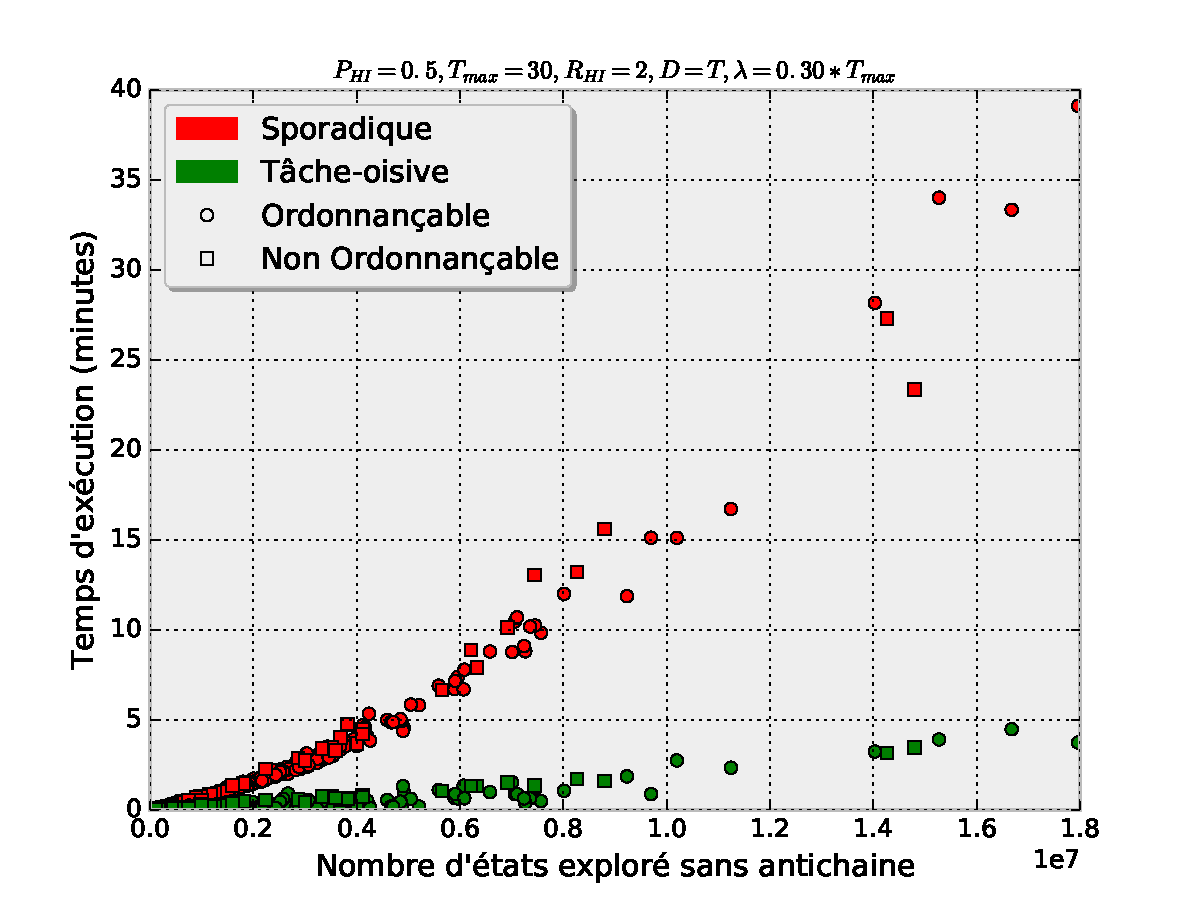
\includegraphics[width=\textwidth]{./results/timeSpoIdle.pdf}
\caption{Analyse de la performance de la relation de simulation}
\label{res:spoIdle}
\end{figure}

\textit{Sporadique : avec antichaîne vs sans antichaîne} : la \autoref{res:spoIdle} compare le temps d'exécution de l'exploration d'un automate généré depuis un système de tâches CM sporadiques jusqu'à arrêt. La comparaison est entre l'exploration avec et sans antichaîne.\\
Chacun des points sur le graphique est un système de tâches CM différent, ceux-ci ont le temps d'exécution qu'il a fallu pour l'explorer, et le nombre d'états explorés sans antichaîne. Les points rouges sont les résultats sans antichaîne, et les verts sont ceux avec antichaîne. De plus, chacun de ces points est rond si le système de tâches CM est effectivement ordonnançable, sinon il est carré.\\
Ces résultats présentent une nette amélioration du temps d'exécution avec une antichaîne.\\

\begin{figure}[h]
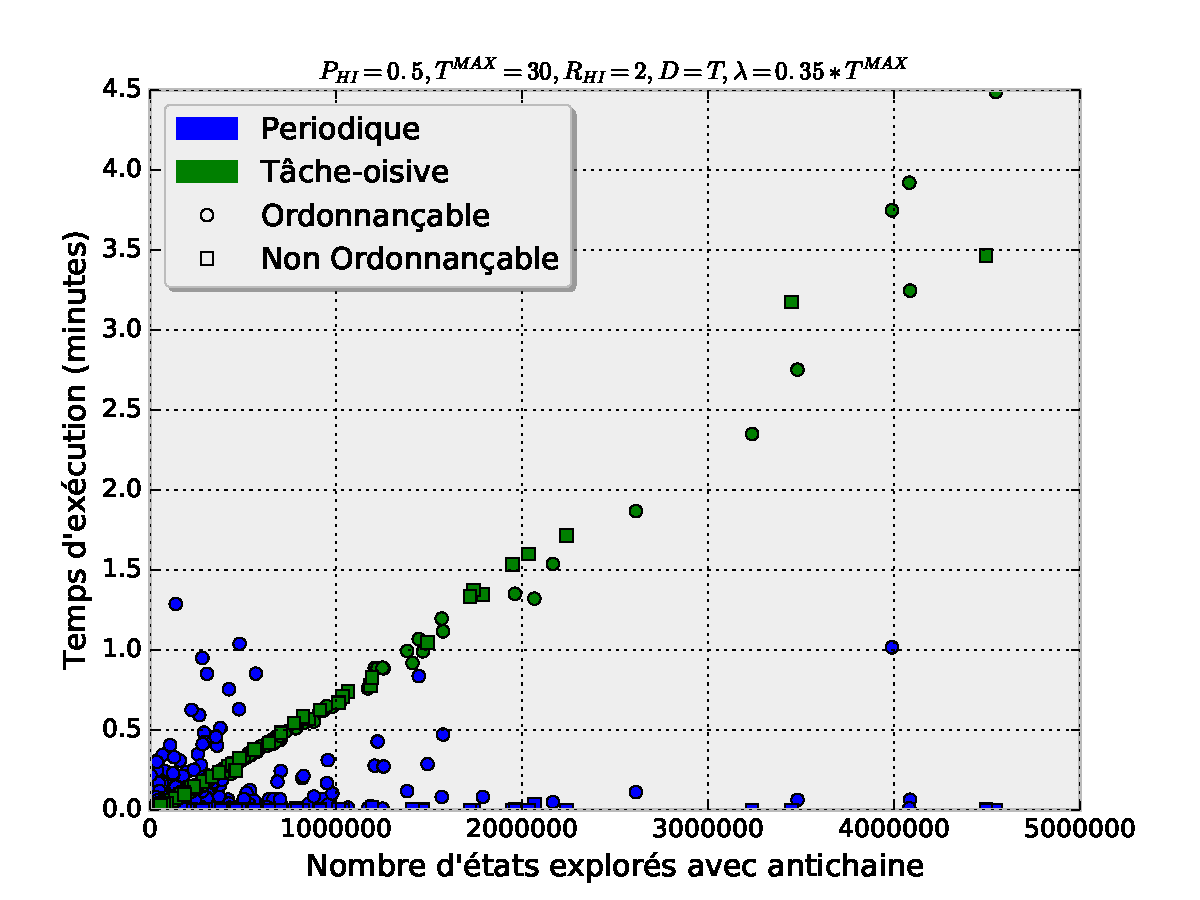
\includegraphics[width=\textwidth]{./results/timePerIdle.pdf}
\caption{Analyse de la performance de la relation de simulation}
\label{res:per-idle}
\end{figure}

\textit{Périodique vs sporadique avec antichaîne} : la \autoref{res:per-idle} compare le temps d'exécution du test d'ordonnançabilité par exploration basé sur tâches CM périodiques et sporadiques avec antichaîne.\\
Ici les points sont tracés sur un graphique du temps d'exécution en fonction du nombre d'états explorés avec antichaîne.\\
Le temps d'exécution de l'exploration pour tâches CM périodiques est parfois supérieur pour les ensembles où l'exploration pour tâches CM sporadiques avec antichaîne prend peu de temps. Ce comportement vient du fait que les antichaînes permettent une représentation efficiente des états et donc l'algorithme peut passer moins de temps à vérifier si un état a déjà été exploré, parce qu'il y en a moins. Mais dès que le système de tâches CM génère un scénario plus compliqué à explorer, il est clair que les tâches CM périodiques génèrent beaucoup moins de cas que les tâches CM sporadiques.\\

\begin{figure}[h]
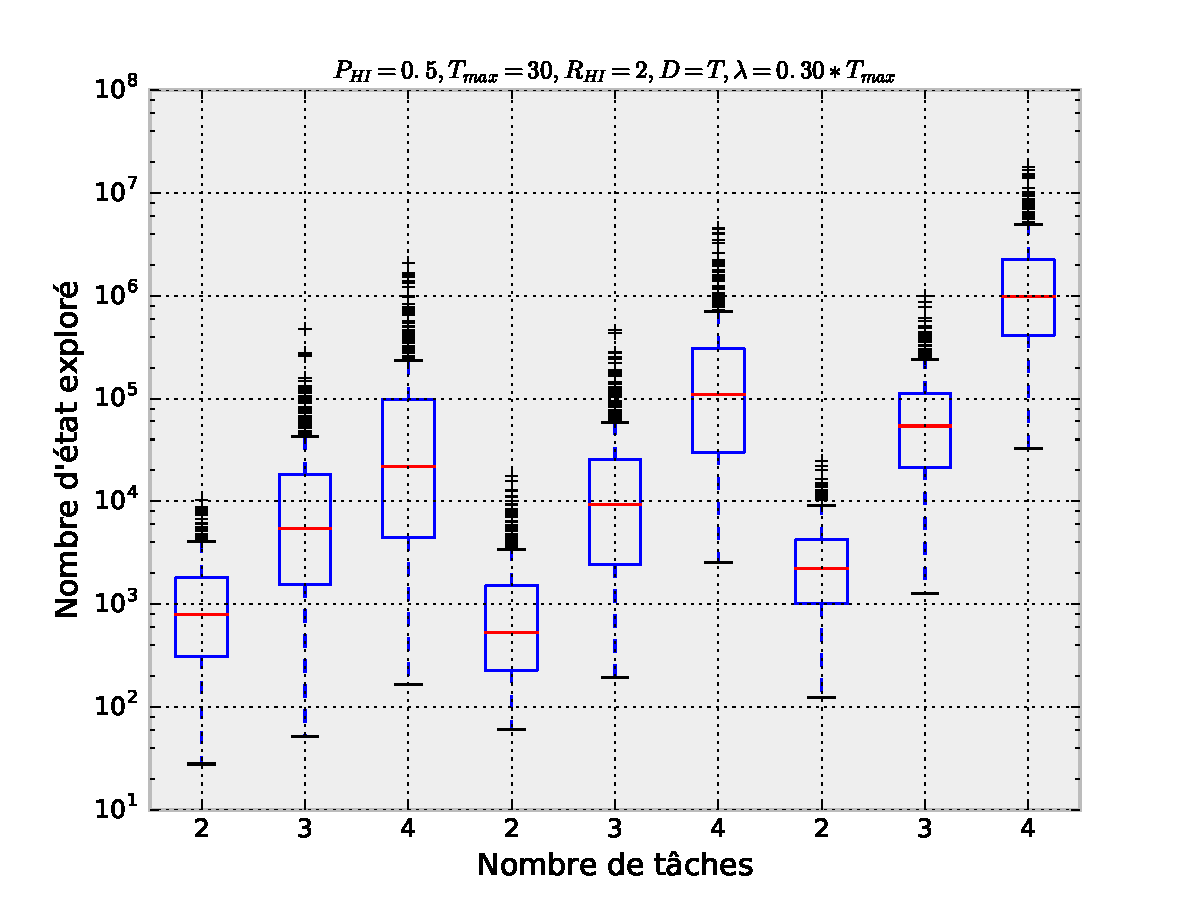
\includegraphics[width=\textwidth]{./results/taskvssize.pdf}
\caption{Taille de l'automate en fonction du nombre de tâches CM}
\label{res:nbetat}
\end{figure}

\textit{Complexité en espace} : sur la \autoref{res:nbetat} on peut lire le nombre d'états visité pour chacun des types d'exploration, pour chaque nombre de tâches CM testé. Il est à noter que l'échelle pour le nombre d'états exploré est logarithmique.\\
Les explorations sont dans l'ordre, périodique, sporadique sans antichaîne, sporadique avec antichaîne.\\
La première observation est que le nombre d'états visité est exponentiel en fonction du nombre de tâches CM présentes dans le système de tâches CM. Pour chacune des tailles des systèmes de tâches CM, l'exploration sporadique avec antichaîne est inférieure à celle sans. L'exploration sporadique avec antichaîne est aussi plus gourmande que la périodique, sauf pour une taille de deux. Cependant, on remarque que la taille de l'automate pour tâches CM sporadiques augmente plus rapidement que celle pour tâches CM périodiques.\\

Ces analyses permettent de visualiser le gain de temps et d'espace net entre l'exploration sporadique avec et sans antichaîne. Comme soupçonné, l'exploration pour tâche CM périodique est bien moins complexe que celle pour tâche CM sporadique même si les antichaînes permettent de réduire cet espace.\\

Dans la suite des résultats, lorsqu'on parlera d'exploration pour tâche CM sporadique, il s'agira toujours de celle avec antichaîne. En effet, celle-ci est moins complexe et mène au même résultat.

\section{Analyse de l'ordonnancement}
Dans cette section, une comparaison de la performance des algorithmes d'ordonnancement pour tâches CM sporadiques est présentée. Dans un premier temps, les différentes versions des algorithmes basés sur le même principe sont comparées. Ensuite, une comparaison générale des algorithmes est analysée.\\

Pour chacun de ces tests, le taux d'ordonnançabilité d'un algorithme est tracé en fonction de l'utilisation du système de tâches CM. Chaque point est le résultat de 2000 simulations, le taux d'ordonnançabilité est alors le nombre de systèmes de tâches CM sporadiques ordonnançables divisé par le nombre total de systèmes de tâches CM testés pour cette utilisation, c'est-à-dire 2000. 41 utilisations sont tracées, il s'agit de $0.4+(x/40)*0.6\ pour\ 0 \le x \le 40,\ x \in \mathbb{N}$. L'utilisation ne va donc pas en dessous de 40\%, d'autres analyses ont montré que le taux d'ordonnançabilité est de 100\% dans de telles conditions \cite{ekberg2012outstanding}.\\

Les systèmes de tâches CM sont générés comme expliqué dans la première section de ce chapitre. Les paramètres de la génération sont $P_{HI} = 0.5, T^{MAX} = 30, R_{HI} = 2, C^{MAX}_{LO} = 15$. Le nombre de tâches CM par ensemble est de 4.\\

\pagebreak

\begin{figure}[h]
\centering
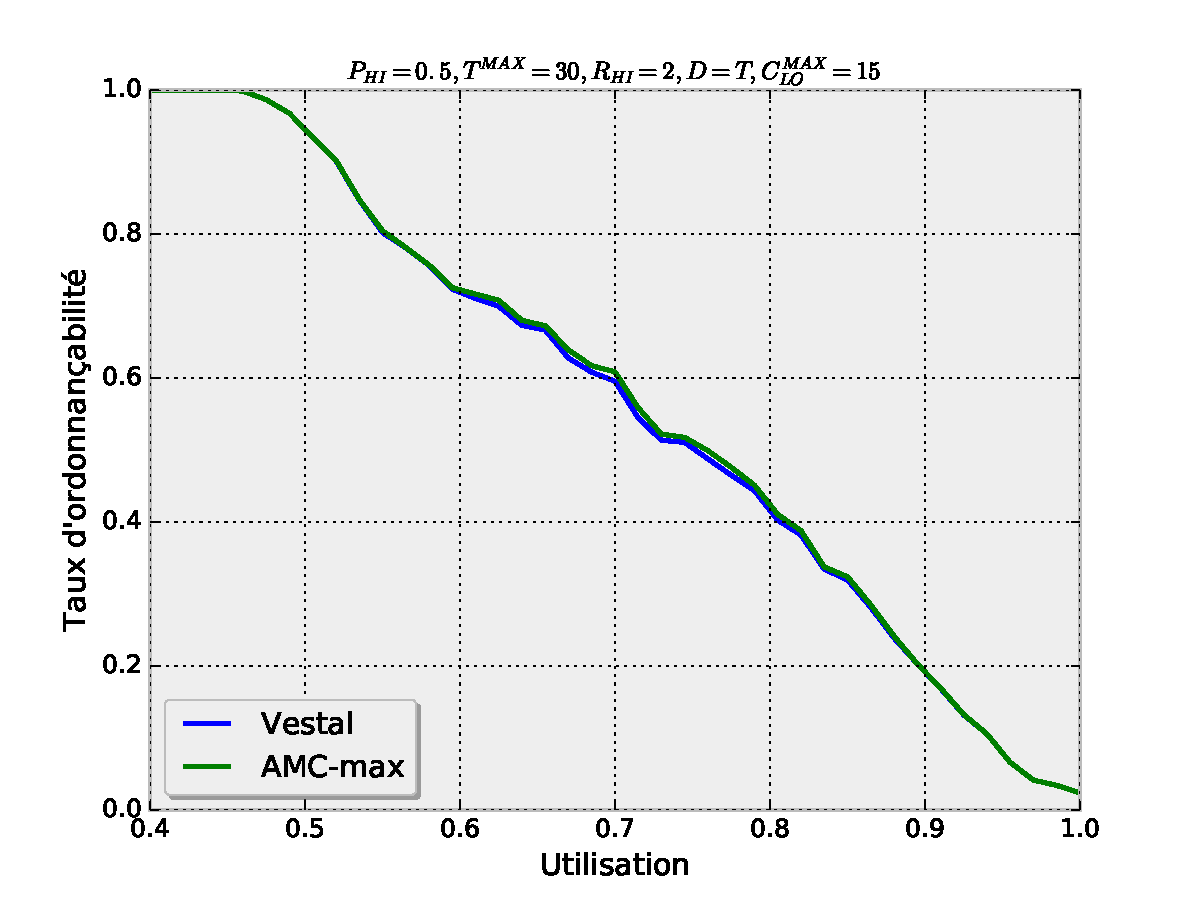
\includegraphics[width=\textwidth]{./results/perfAMCVestal.pdf}
\caption{Ordonnançabilité de Vestal et AMC-max}
\label{res:vestalamc}
\end{figure}

\textit{Vestal vs AMC-max} : la \autoref{res:vestalamc} compare l'ordonnançabilité de \textit{Vestal} et \textit{AMC-max}, basée sur leur assignation de priorité initiale présentée en \autoref{vestal}.\\
Ici l'algorithme \textit{AMC-max} borne supérieurement les résultats de \textit{Vestal}. \textit{AMC-max} ayant une condition pour vérifier qu'une tâche CM peut recevoir une certaine priorité plus laxiste que celle de \textit{Vestal}, ce résultat est celui attendu.\\

\pagebreak

\begin{figure}[h]
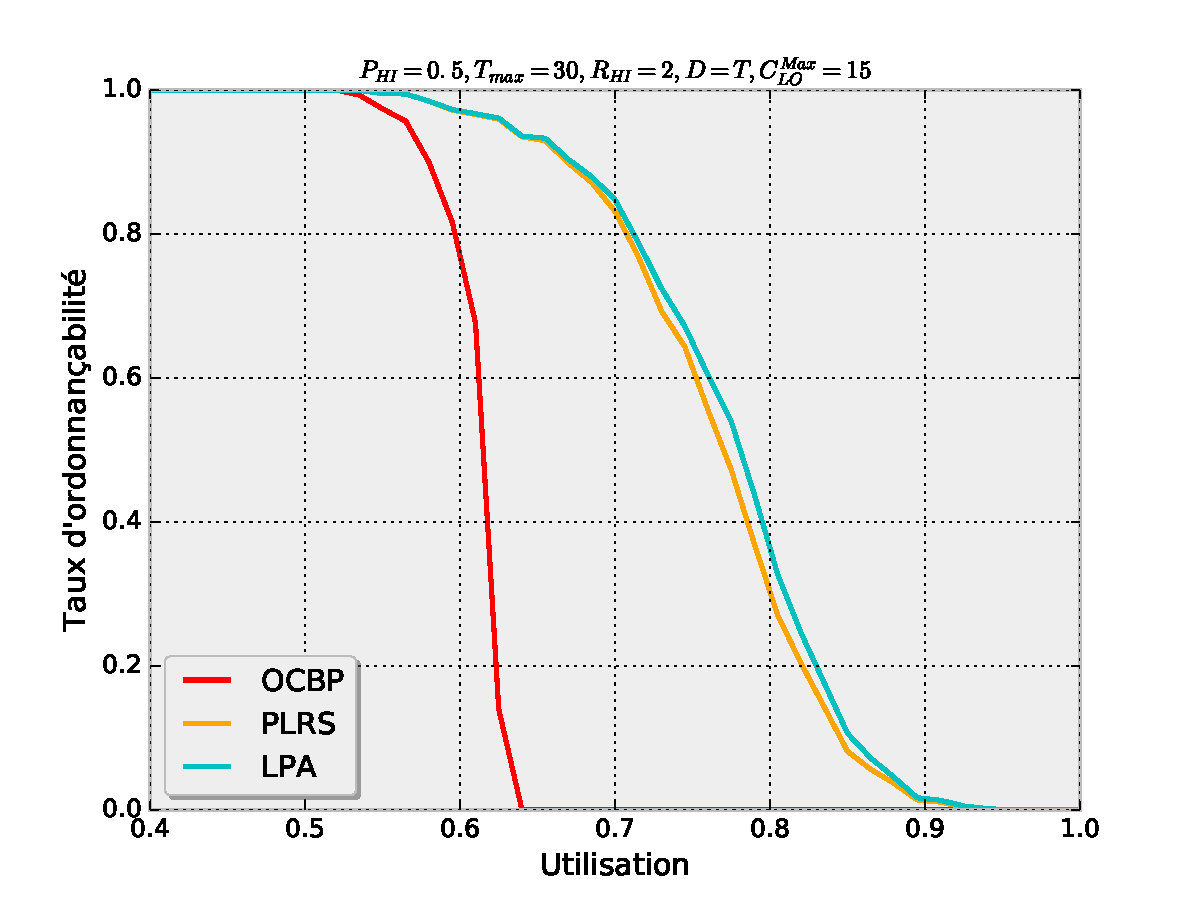
\includegraphics[width=\textwidth]{./results/perfOCBPetc.pdf}
\caption{Ordonnançabilité de OCBP et extensions}
\label{res:ocbpbext}
\end{figure}

\textit{OCBP et extensions} : la \autoref{res:ocbpbext} compare les performances de \textit{OCBP} et de ses extensions \textit{PLRS} et \textit{LPA}.\\
Le test d'\textit{OCBP} basé sur la charge d'un système de tâches CM est clairement plus pessimiste que celui des deux autres, basés sur une assignation de priorité initiale présentée en \autoref{plrslpa}.\\

En comparant l'ordonnançabilité de \textit{PLRS} et \textit{LPA}, \textit{LPA} offre un résultat légèrement meilleur. L'inverse serait étonnant, car \textit{LPA} a la même assignation de priorité que \textit{PLRS}, sauf que \textit{LPA} borne le plus grand intervalle occupé avec plus de précision que \textit{PLRS}, menant à moins d'échecs d'assignation.\\

\pagebreak

\begin{figure}[h]
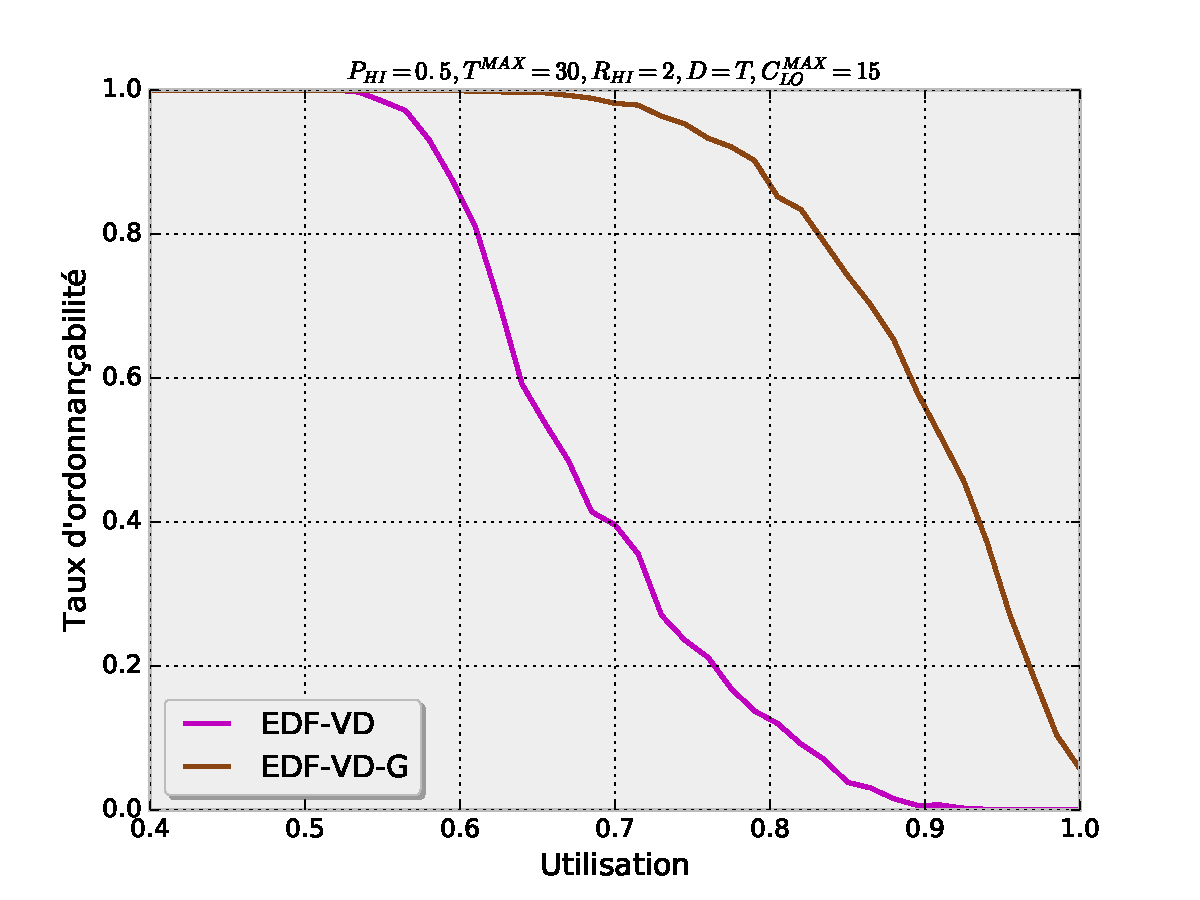
\includegraphics[width=\textwidth]{./results/perfEDFVD.pdf}
\caption{Ordonnançabilité de EDF-VD}
\label{res:edfvd}
\end{figure}

\textit{EDF-VD} : la \autoref{res:edfvd} compare le test d'ordonnancement préalable de \textit{EDF-VD} basé sur l'utilisation à différents niveaux de criticité et l'ordonnançabilité réelle de l'algorithme, définie grâce à la réduction de cette question vers l'exploration d'un automate. Lorsque \textit{EDF-VD} est utilisé pour l'exploration d'un automate, le cas 2 (\textit{cf.} \autoref{edfvd}) est utilisé même si la condition n'est pas respectée.\\

La différence entre le test d'ordonnançabilité préalable et l'ordonnançabilité réelle de \textit{EDF-VD} est flagrante. L'ordonnançabilité de \textit{EDF-VD} est bien plus grande que celle qui était connue jusqu'à présent.\\

\pagebreak

\begin{figure}[h]
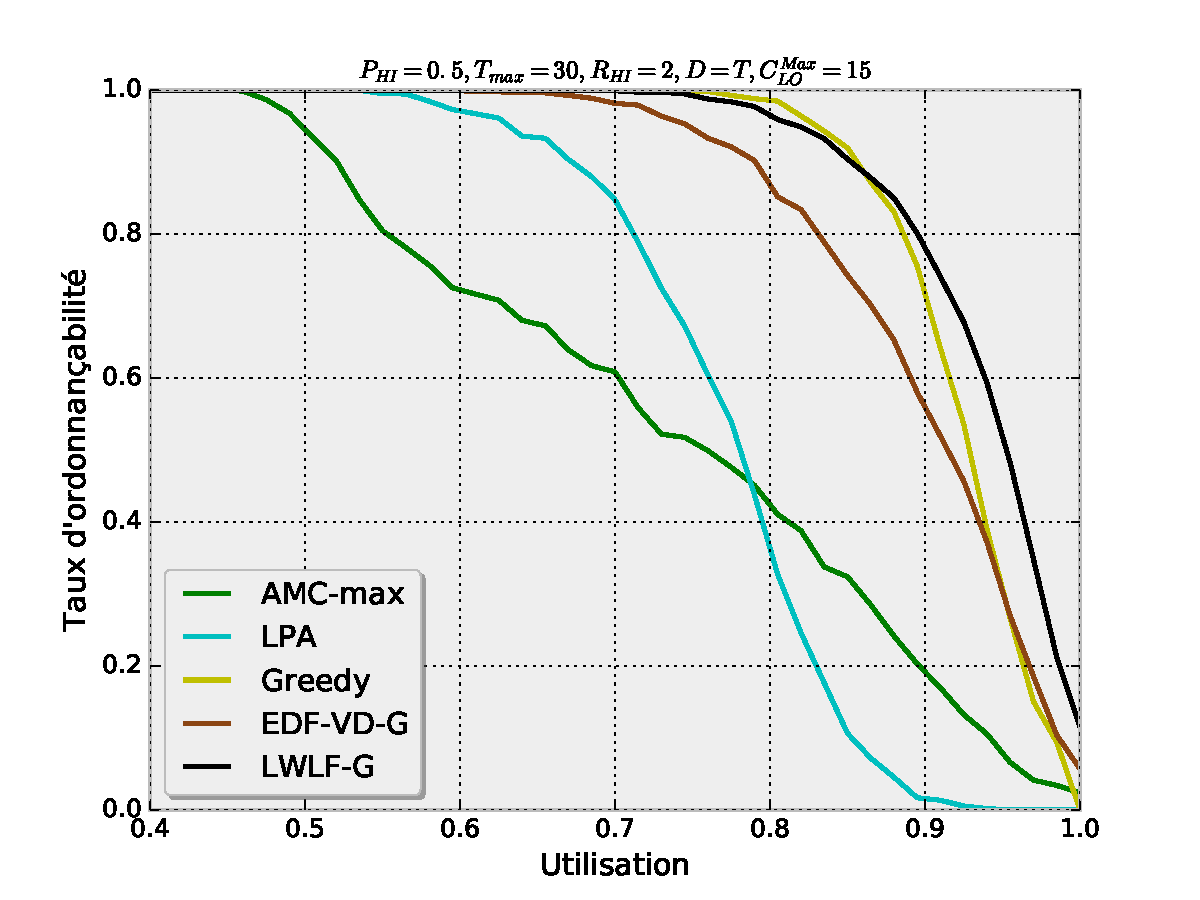
\includegraphics[width=\textwidth]{./results/perfComp.pdf}
\caption{Comparaison des algorithmes}
\label{res:full}
\end{figure}

\textit{Comparaison générale} : la \autoref{res:full} compare les différents algorithmes entre eux. Les versions les plus optimisées, et les meilleurs tests sont utilisés. Pour l'algorithme \textit{Greedy}, le taux d'ordonnançabilité à 100\% est placé arbitrairement à 0, car le calcul utilisé pour déterminer $\Delta$ requiert que l'utilisation soit inférieure à $1$.\\

\textit{AMC-max} donne le plus mauvais résultat jusqu'à une utilisation à 80\% où \textit{LPA} prend alors la relève. \textit{LPA} base son test notamment sur le calcul de la plus grande période occupée et celle-ci est calculée à partir de l'utilisation du système de tâches CM. Lorsque cette utilisation est égale à 1, la plus grande période occupée est alors infinie, et cet algorithme est inutilisable. Ensuite vient \textit{EDF-VD}, qui borne les deux précédents algorithmes. Puis \textit{Greedy} et \textit{LWLF} s'entremêlent. L'ordonnançabilité de \textit{LWLF} est calculée grâce à la réduction de l'ordonnançabilité vers l'accessibilité dans un automate. \textit{Greedy} et \textit{LWLF} ont un taux d'ordonnançabilité identique jusqu'à $75\%$, ensuite \textit{Greedy} domine jusqu'à environ $85\%$, où \textit{LWLF} reprend le dessus.

\chapter{Conclusion}
\label{chap:ccl}
Ce mémoire a commencé par définir l'ordonnancement en criticité mixte, par expliquer son importance et celle de son test. En deuxième lieu, il a été proposé de réduire ce problème vers celui de l'accessibilité dans un automate. Les notions nécessaires à la compréhension de ce second problème ont été données. Ensuite, la notion d'antichaîne et de relation de simulation ont été expliquées, ainsi que l'amélioration qu'elles apportent à l'accessibilité dans un automate.\\

La seconde partie du travail regroupait les différents algorithmes d'ordonnancement d'un système de tâches CM sporadiques, en donnant leur fonctionnement général et leur test d'ordonnançabilité. En plus de ces algorithmes venant de la littérature, l'algorithme original \textit{LWLF} a été proposé.\\

La troisième partie du mémoire a décrit comment réduire l'ordonnançabilité CM vers l'accessibilité dans un automate, apportant le test d'ordonnançabilité CM exact pour un algorithme. Deux problèmes ont été réduits, celui concernant les systèmes de tâches CM périodiques et celui pour les systèmes de tâches CM sporadiques. Enfin, cette partie a proposé la relation de simulation de tâches oisives pour les systèmes de tâches CM sporadiques.\\

Tout ce travail a permis de comparer les taux d'ordonnançabilité CM de différents algorithmes, mais avant d'en tirer des conclusions, il faut déjà apprécier l'outil en lui-même, et le gain que les antichaînes lui apportent.\\

En effet, l'ajout d'une antichaîne à l'automate a permis de gagner un temps considérable durant l'exploration. De plus, la relation de simulation de tâches oisives semble pouvoir être exportée pour différents types d'ordonnancement lors de l'utilisation de tâches CM sporadiques, comme c'est le cas pour l'ordonnancement classique sur multiprocesseur \cite{geeraerts2013multiprocessor}.\\

De plus, la création de ce test d'ordonnançabilité CM exacte démocratise le problème dont il est issu. L'ordonnançabilité en criticité mixte selon un algorithme pourrait alors devenir lui-même un problème vers lequel un autre est réduit.\\

Enfin, cette réduction de problème est un canal entre deux domaines des sciences informatiques. Utiliser des outils interdisciplinaires est toujours souhaitable, car cela permet de résoudre plus de problèmes et cette démarche est une réussite pour ce travail.\\

Lors de la comparaison de l'ordonnançabilité des algorithmes entre eux, on s'aperçoit que les trois meilleurs sont \textit{Greedy}, \textit{LWLF} et \textit{EDF-VD}.\\
\textit{Greedy} donne une très bonne ordonnançabilité, c'est intéressant, car il est basé sur un test en temps polynomial. En revanche, l'algorithme \textit{LWLF} est plus puissant que \textit{Greedy} pour des systèmes de tâche CM à haute utilisation.\\

Ce dernier résultat est très intéressant, car il montre qu'avec l'outil créé dans ce mémoire, il sera possible de tester toute une série d'algorithmes issue de l'imagination, sans pour autant directement devoir trouver une condition suffisante d'ordonnançabilité théorique. Ce qui a été le cas pour \textit{LWLF} et cet algorithme, basé sur une simple intuition, donne l'un des meilleurs résultats.\\

\paragraph{Travaux ultérieurs}
Pour continuer dans le développement du travail effectué dans ce mémoire, une première étape serait de développer une implémentation de la réduction proposée en un langage plus optimisé, tel que \textit{c++}. Cette approche n'a pas été suivie ici, car l'approche utilisée a fonctionné sur essais et erreurs, par recherche.\\
Un gain dans la complexité en temps permettrait de faire des analyses plus poussées du taux d'ordonnançabilité d'algorithmes, telles que faire varier les différents paramètres de création de systèmes de tâches CM ($T^{MAX}, R_{HI}$ ...), tester avec des systèmes de tâches CM plus grands, avec plus de niveaux de criticités, avec des échéances arbitraires.\\

Un futur travail pourrait aussi explorer la création d'autres relations de simulations. Des pistes infructueuses sont données à la fin du chapitre présentant la relation de simulation de tâches oisives.\\

Ce mémoire a proposé l'algorithme \textit{LWLF} qui a donné de bons résultats. Continuer à explorer cet algorithme permettrait peut-être de trouver une condition suffisante d'ordonnançabilité à complexité polynomiale par exemple.\\

En possession d'un tel test d'ordonnançabilité exact, il est possible d'imaginer une série de nouveaux algorithmes et de tester leur potentiel rapidement. Cet outil peut alors aider la conception d'un hypothétique algorithme optimal pour l'ordonnancement CM.\\

Enfin, pour obtenir un test d'ordonnançabilité CM indépendant d'un algorithme d'ordonnancement, il faudrait envisager de créer un jeu d'accessibilité basé sur l'automate présenté dans ce mémoire. L'agent aurait le pouvoir sur la tâche CM que l'ordonnanceur sélectionne, le reste ferait partie de l'environnement. Il s'agirait alors de voir s'il est possible de trouver une stratégie gagnante et si oui, alors le système de tâches CM sur lequel est basé l'automate est ordonnançable CM.

\appendix


\chapter{Implémentation en Python 3}
\section{Modèles de donnés}

\subsection{Tâche CM}
\printcode{./code/Task.py}

\subsection{Système de Tâches CM}
\printcode{./code/TaskSet.py}

\section{Test d'ordonnançabilité CM}
\subsection{Vestal}
\printcode{./code/sufficientCond/Vestal.py}

\subsection{AMC-max}
\printcode{./code/sufficientCond/AMCmax.py}

\subsection{OCBP}
\printcode{./code/sufficientCond/OCBP.py}

\subsection{PLRS}
\printcode{./code/sufficientCond/PLRS.py}

\subsection{LPA}
\printcode{./code/sufficientCond/LPA.py}

\subsection{EDF-VD}
\printcode{./code/sufficientCond/EDFVD.py}

\subsection{Greedy}
\printcode{./code/sufficientCond/Greedy.py}

\section{Automate périodique}
\subsection{Etat du système}
\printcode{./code/PeriodicSystemState.py}

\subsection{Exploration}
\printcode{./code/PeriodicGraph.py}


\section{Automate sporadique}
\subsection{Etat du système}
\printcode{./code/SporadicSystemState.py}

\subsection{Exploration}
\printcode{./code/SporadicGraph.py}

\subsection{Antichaîne}
\printcode{./code/SporadicMaxSet.py}

%\nocite{*}
\bibliographystyle{unsrt}
%\bibliographystyle{plain}
\bibliography{./reference/bibliography}

\printindex


\end{document}

